\documentclass[11pt]{psuthesis}
\usepackage{amsmath,amssymb,marvosym,wasysym}
\usepackage{natbib}
\usepackage{psfig,graphics,graphicx} 
\usepackage{deluxetable}
\usepackage{longtable}		% FOR DISPLAYING MULTI-PAGE TABLES
\usepackage{lscape}
\usepackage[usenames, dvipsnames]{color}
\usepackage{url}
\usepackage{rotating}
\usepackage{longtable}
\usepackage[caption=false]{subfig}
\usepackage{float}
\usepackage{morefloats}
\usepackage{ulem}
\usepackage{tabularx}
\usepackage{verbatim} % for long comments
\usepackage{array} % for line-wrapping table
\newcolumntype{L}{>{\arraybackslash}m{3cm}}
% for pretty refs - Oops! this breaks the list of figures
%\usepackage[colorlinks,urlcolor=black,citecolor=black,linkcolor=black]{hyperref}


\bibpunct{(}{)}{;}{a}{}{,}
\def\apj{ApJ}
\def\aaps{A\&AS}
\def\aap{A\&A}
\def\apjl{ApJ}
\def\aj{AJ}
\def\araa{ARA\&A}
\def\pasp{PASP}
\def\mnras{MNRAS}
\def\nat{Nature}
\def\apjs{ApJS}
\def\aapr{A\&A~Rev.}


\definecolor{Blue}{rgb}{0.,0.,1.0}
\definecolor{Red}{rgb}{1.,0.,.0}

\makeatletter
\newcommand{\rom}[1]{\romannumeral #1}
\newcommand{\Rom}[1]{\expandafter\@slowromancap\romannumeral #1@}
\makeatother


\newcommand{\ion}[2]{[#1$\;${\scriptsize\Rom{#2}}]}
\newcommand{\ionl}[3]{[#1$\;${\scriptsize\Rom{#2}}]\relax$\lambda$#3}
\newcommand{\ionr}[2]{\rm[#1\;{\scriptsize\Rom{#2}}]}
\newcommand{\ionm}[2]{[#1\;{\scriptsize\Rom{#2}}]}

\newcommand\arcsec{\mbox{$^{\prime\prime}$}}%
\def \arcsecond#1#2{$#1\arcsec\!\!.#2$}
\newcommand\farcs{\mbox{$.\!\!^{\prime\prime}$}}%

%%%%%%%%%% command for URL-like text
\newcommand{\link}[1]{{\color{Blue}\uline{#1}}}


%%% section titles
\newcommand{\header}[1]{{\noindent\textsc{\textbf{\textsc{\large#1}}}}}
\newcommand{\topic}[1]{
  \raggedright
  \noindent\rule[-8mm]{16cm}{0.2mm}\\
  \noindent\rule{16cm}{0.2mm}\\
  \header{#1}
}

%%% item commands
\newcommand{\quadrupleitem}[4]{
  \begin{tabularx}{\textwidth}{Xr}
  {\bf #1}            & #2\\
   #3            & #4\\
  \end{tabularx}
}
\newcommand{\tripleitem}[3]{
  \raggedleft
  \begin{tabularx}{\textwidth}{Xr}
  {\it #1}            & #2\\
  #3 & \\
  \end{tabularx}
}
\newcommand{\doubleitem}[2]{
  \raggedleft
  \begin{tabularx}{\textwidth}{Xr}
  {\bf #1}            & #2\\
  \end{tabularx}
}
\newcommand{\doubleitemnobold}[2]{
  \raggedleft
  \begin{tabularx}{\textwidth}{Xr}
  #1 & #2\\
  \end{tabularx}
}



% above: a mixture of original and Jason's
%%%%%%%%%%%%%%%%%%%%%%%%%%%%%%%%%%%%%%%%%%%%%%%%%%%%%%%%%%%%%%%%%%%
% Sharon's customized
%%%%%%%%%%%%%%%%%%%%%%%%%%%%%%%%%%%%%%%%%%%%%%%%%%%%%%%%%%%%%%%%%%%
% general commands and texts
\newcommand{\beq}{\begin{equation}}
\newcommand{\eeq}{\end{equation}}
\def\etal{~et~al.~}

% math
\def\mps{m/s}
\def\msini{M\sin{i}}
\def\chisq{$\chi_{\nu}^2$}
\def\degree{^{\circ}}
\def\leq{\leqslant}
\def\geq{\geqslant}

% planets
\def\mjup{M_{\rm Jup}}
\def\msol{M_{\odot}}
\def\mearth{M_{\oplus}}
\def\rearth{R_{\oplus}}

% astro acronyms
\def\kepler{{\it Kepler}}
\def\spitzer{{\it Spitzer}}
\def\minerva{MINERVA}
\def\hrs{HET/HRS}
\def\keck{Keck/HIRES}
\def\epds{WIYN/EPDS}
\def\harps{HARPS-N}
\def\rvlin{{\tt RVLIN}}
\def\boottran{{\tt BOOTTRAN}}




\begin{document}

\title{On Detecting New Worlds: \\
  The Art of Precise Doppler Spectroscopy \\
  Using Iodine Cells}
\author{Sharon Xuesong Wang}
\dept{The Department of Astronomy and Astrophysics}
\degreedate{August 2016}
\copyrightyear{2016}


\begin{singlespace}

\numberofreaders{5}
\advisor[Dissertation Advisor, Chair of Committee]
        {Jason T.\ Wright}
        {Associate Professor of Astronomy and Astrophysics}

\readerone{Suvrath Mahadevan}
          {Associate Professor of Astronomy and Astrophysics}

\readertwo{Lawrence Ramsey}
          {Distinguished Senior Scholar and Professor of Astronomy}

\readerthree{Eric Ford}
            {Professor of Astronomy and Astrophysics}

\readerfour{James Kasting}
           {Evan Pugh Professor of Geosciences}

\readerfive{Michael Eracleous}
           {Professor of Astronomy and Astrophysics, Head of Graduate Program}

\begin{frontmatter}


\begin{doublespace}

\frontmatter
\psutitlepage
\psucommitteepage
\thesisabstract{abstract}
\thesistableofcontents
\thesislistoffigures
\thesislistoftables
\end{doublespace}


\clearpage
\thesisacknowledgments{acknowledgements}
\end{frontmatter}

\thesismainmatter
\allowdisplaybreaks{
\chapter{Introduction}

\begin{quote}
``There are infinite worlds both like and unlike this world of
ours. For the atoms being infinite in number, as was already proven,
...there nowhere exists an obstacle to the infinite number of worlds.''
\end{quote}
\hfill Epicurus ($\sim$341-270 B.C.)

\begin{comment}
\begin{quote}
``This space we declare to be infinite... In it are an infinity of
worlds of the same kind as our own.''
\end{quote}
\hfill Giordano Bruno, {\it On the Inifinite Universe and Worlds} (1584)
\end{comment}

\begin{quote}
``How vast those Orbs must be, and how inconsiderable this Earth, the
Theatre upon which all our mighty Designs, all our Navigations, and
all our Wars are transacted, is when compared to them.''
\end{quote}
\hfill Christiaan Huygens, {\it Cosmotheoros} (1698)

\begin{quote}
``Of all of the topics of study in astronomy, exoplanets hold a
special place in the imagination. More than stars, nebulae, or
galaxies, they are {\it places}, ...''
\end{quote}
\hfill \cite{2006PhDT.........8W}

%%%%%%%%%%%%%%%%%%%%%%%%%%%%%%%%%%%%%%%%%%%%%%%%%%%%%%%%%%%%%%%%%%%%%%%%%%%%%%
\section{On Detecting New Worlds}

Even before human beings realized that other stars are like our Sun,
the existence of other worlds have been speculated by ancient greek
philosophers such as Epicurus and Democritus. In the blooming age of
astronomy in the 1400s and 1600s, early pioneers such as Giordano
Bruno and Christiaan Huygens have also pondered upon the existence of
planets around other stars (extra-solar planets, or
exoplanets).\footnote{In fact, Huygens conducted the first documented
search on exoplanets. For more on the history of exoplanet searches,
see these three websites:\\ The NASA PlanetQuest,
http://www.nasa.gov/externalflash/PQTimeline/; \\ Search for
Exoplanets, http://www.hao.ucar.edu/research/stare/search.html; \\
ESO,
https://www.eso.org/public/outreach/eduoff/cas/cas2004/casreports-2004/rep-228/. }
In modern times, 40 years before the discovery of the first exoplanet,
Otto Struve stated that exoplanets, especially ``super-Jupiters'' on
short orbits, should be detectable via spectroscopy and photometry
\citep{1952Obs....72..199S}.

Unfortunately, the earliest claims of exoplanet detections before
1980s all turned out to be erroneous \citep{1855MNRAS..15..228J,
1969AJ.....74..757V}. These and a later retracted claim of a planet
around a pulsar by \cite{1991Natur.352..311B} made all astronomers
extremely cautious about exoplanet detection claims. In 1988,
Campbell, Walker and Yang announced potential planetary signal from
the star Gamma Cephei, but they were hesitant in calling it a
detection due to limitations of early instruments. Their detection
method was to measure the radial velocity (RV) variation of the star
using precise Doppler spectroscopy, which is described in the next
section and is also the theme of this thesis.  It was not until 2003
that the planet around $\gamma$ Cephei A was confirmed
\citep{2003ApJ...599.1383H}, which made the work of
\cite{1988ApJ...331..902C} the first exoplanet detection. The
detection of HD 114762b (``Latham Planet'';
\citealt{1989Natur.339...38L}) also belongs to the family of first
exoplanet detections, though the planet was thought to be a brown
dwarf at the time due to its large mass. A similar story to $\gamma$
Cephei Ab is the discovery of $\beta$ Gemini b
\citep{1993ApJ...413..339H}, where the existence of the planet was not
confirmed until 2006 \citep{2006A&A...457..335H} because of the strong
activity-induced RV signals of the giant host star.\footnote{See
  Chapter 4 of \cite{2013pss3.book..489W} for a more detailed history
  on these early detections.} 

The more commonly recognized first detection of exoplanets belongs to
\cite{1993ApJ...413..339H}, who reported two planets around the pulsar
PSR B1257$+$12, detected via the pulsar timing method using radio data
(later on it turned out this system hosts one more planet). It was a
surprising detection in many aspects, and these planets remains the
only known planetary system around a pulsar to date (as of May
2016). If exoplanets could exist around exotic stars like pulsars,
then it is only natural to expect them to exist around more
``regular'' main-sequence stars like our Sun.

Finally, in 1995, a team in Geneva announced the first definitive
detection of a planet around a main-sequence star, 51 Peg b
\citep{1995Natur.378..355M}. Their results were quickly confirmed by
other planet hunters such as Geoffrey W.\ Marcy and R.\ Paul Butler,
who quickly caught up with the game \citep{1996ApJ...464L.153B} and
went on to detect more than half of the hundreds of known exoplanets
up until the launch of NASA's \kepler\ mission
\cite{2010Sci...327..977B}. The method adopted by
\cite{1995Natur.378..355M} and \cite{1996ApJ...464L.153B} was again
precise Doppler spectroscopy. Today, there are over 585 exoplanets
discovered by precise Doppler spectroscopy. The discoveries by precise
Doppler spectroscopy that happened beyond this point is briefly
accounted for in the next section. 

Several years later, \cite{2000ApJ...529L..41H} and
\cite{2000ApJ...529L..45C} detected the first exoplanet transiting
event, where the planet moves in between the disk of the star and our
line of sight periodically, leaving signals in the stellar light
curves. This transiting planet, HD
209458b, which was discovered via precise Doppler spectroscopy
first. Nonetheless, this discovery opened up the age of ground-based
transit, where projects such as OGLE, TrES, WASP, XO, and HAT etc.\ added
more than 200 new exoplanet discoveries to date
\citep{2003Natur.421..507K, 2004ApJ...613L.153A, 2006MNRAS.372.1117C,
  2006ApJ...648.1228M, 2007ApJ...656..552B}. 

In 2009, the discovery of exoplanets entered a new era with the launch
of NASA's \kepler\ satellite, which is a dedicated space mission to
detect transiting exoplanets. This extremely fruitful mission has made
new exoplanet discoveries in the counts of thousands
\citep{2014ApJ...784...45R, 2016ApJ...822...86M}, with over 2000 more
planet candidates (see, e.g., NASA Exoplanet Archive for statistics on
exoplanet discoveries). The science of exoplanets expanded from the
philatelic style to including population and statistical studies which
inform planet formation and evolution in powerful ways more than ever
(e.g., \citealt{2013ApJ...766...81F} on occurrence rate and
\citealt{2015arXiv150407557W} on composition distribution). As of May
23 2016, there are 3268 confirmed exoplanets, to which the transit
method contributed 2569 (585 discovered by Doppler spectroscopy).

Besides using precise Doppler spectroscopy and transits, other methods
have also made unique and important discoveries of exoplanets, as they
probe different stellar population and are subject to different
observational biases. \cite{2004ApJ...606L.155B} made the first
micro-lensing detection of exoplanet, where planets acts as additional
gravitational lenses beside their host star and leave characteristic
signatures onto the light curves of the background star. There are 37
exoplanets discovered via micro-lensing so far. Astronomers also
directly detected light from young exoplanets around young stars via
direct imaging, the first of which are Fomalhaut b
\citep{2008Sci...322.1345K} and the four planets around HR 8799
\citep{2008Sci...322.1348M}. Today, there are 41 directly imaged
planets.

More exoplanets around more diverse host stars are expected to be
discovered in the near future, with many new missions and surveys
being carried out, built, or planned. Post-2013, \kepler\ continued as
the K2 mission (\kepler\ on two reaction wheels) and kept churning out
planets (e.g., \citealt{2016ApJS..222...14V}). The Transiting
Exoplanet Survey Satellite (TESS; \citealt{2014SPIE.9143E..20R};
expected to launch in Summer 2017) will survey the whole sky,
targeting nearby and bright stars, including the previously relatively
unexplored population of M dwarf stars. There is no doubt that, once
again, exoplanet discoveries will be made in counts of
thousands. Ongoing surveys with the Gemini Planet Imager on Gemini
South \citep{2014PNAS..11112661M} and the SPHERE instrument on the
Very Large Telescope \citep{2008SPIE.7014E..18B} are populating
exoplanets in a new parameter space (young stellar/planetary age and
moderate to long orbital distances). The future for micro-lensing
discoveries also remains bright as thousands of exoplanets are
expected to be found by NASA's WFIRST-AFTA mission
\citep{2014arXiv1409.2759Y}.

Among all these exciting discoveries happening or on the horizon,
precise Doppler spectroscopy continues to play an important role. It
is the most important method for measuring planetary
masses,\footnote{Planetary masses can also be measured via studies on
the transit timing variations (TTVs) due to the dynamic interactions
of multiple planets (e.g., \citealt{2016ApJ...820...39J}), but TTVs
are only measurable for a small fraction of all transiting planets
\citep{mazeh2013}. \cite{2013Sci...342.1473D} have also developed an
innovative method to estimate planetary mass via transmission
spectroscopy of the planetary atmosphere, but the method is
model-dependent and requires a large amount of large-aperture space
telescope time (e.g., hundreds of orbits of JWST).} and it will remain
a crucial independent method for discovering new exoplanets (after
all, only a small fraction of exoplanets happen to pass in between
their host star and the Earth). The synergy between the \kepler\
mission and the ground-based Doppler spectroscopy follow-ups has
demonstrated the power of this new exoplanet discovery and
characterization ``routine'', where RVs are presented as the
convincing evidence for the planetary nature of the transit signal,
and they also provide valuable information on the planetary masses and
thus their bulk densities (e.g., \citealt{marcy2014}). Such
measurements are crucial for mapping out the demographics of
exoplanets. However, only a small fraction of \kepler\ targets have
been followed up by Doppler spectroscopy, and the future discoveries
of TESS will put an even higher demand on RV follow up (see, e.g.,
a summary in \citealt{exopag2015}).

Doppler spectroscopy also remains the most promising avenue for
detecting Earth-like planet in the Habitable Zone
\citep{1993Icar..101..108K, 2013ApJ...765..131K} in the near
future. Figure~\ref{intro:fig:hz} illustrates the Habitable Zones for
different types of stars and the discovery space that TESS will
access, which does not include the Habitable Zone around Sun-like to
early-M stars due to TESS's short lifespan. The next generation
Doppler spectroscopy, with a RV precision of $<$0.5~m/s, bears great
hope for detecting rocky or even Earth-like planets in the Habitable
Zone. Can we fulfill such a great expectation? The next section
focuses on the art of precise Doppler spectroscopy, on how we achieved
the current precision of 1~m/s today, and on how the field will carry
on and aim for a RV precision of $\sim 10$~cm/s in the coming decade.


%----------------------------------------------------------------
% stellar T vs. planet period, showing RV amplitude curves
% plot provided by Paul Robertson, converted online to eps
\begin{figure}
\centering
\includegraphics[scale=0.55]{introduction/habitable_zone.eps}
\caption{Habitable Zone for stars with various effective temperature,
  highlighted in blue (and red for the extended zone). Some known
  planets in the Habitable Zone of their host stars are plotted, scaled
  by their sizes. Solar system planets are also plotted and scaled by
  size. The yellow and orange dashed vertical lines mark the discovery
  space in terms of planetary periods that TESS is most sensitive
  to. The white curves are equal-RV-amplitude lines, showing the
  semi-amplitude of the RV signals induced by any hypothetical
  Earth-mass planets on each curve. This plot is made by Chester Harman
  and Ravi Kopparapu and kindly provided by Paul Robertson.
\label{intro:fig:hz}}
\end{figure}
%----------------------------------------------------------------



%%%%%%%%%%%%%%%%%%%%%%%%%%%%%%%%%%%%%%%%%%%%%%%%%%%%%%%%%%%%%%%%%%%%%%%%%%%%%%
\section{The Art of Precise Doppler Spectroscopy}

History of precise Doppler spectroscopy. Early work by Campbell and
Walker. First detections with ThAr. Quickly progressed to 3m/s with
iodine. HARPS revoluntionized the field by showing what a cryogenic 
spectrometer can do. Poor NIR...

What is the landscape of RV instruments today. Table of current instruments.

Figure of current precision.

The current best RV precision is around 1~m/s \citep{eprv2015},
attainable via two wavelength calibration methods in the optical band:
ThAr lamp emission line calibration (e.g., ELODIE and HARPS;
\citealt{elodie, harps-s}; $\sim$400-690~nm) and iodine cell
absorption line calibration (e.g., Keck/HIRES and Magellan/PFS;
\citealt{butler1996, 2010SPIE.7735E..53C}; $\sim$500-620~nm). The
major obstacles for achieving a higher RV precision are: stellar
activity induced RV signals, instrumental effects, telluric
contamination, and limitation in data analysis \citep{eprv2015}.

Where is the field heading towards in the near future. Fischer et
al. review, Plavchan NASA white paper. 

Table of Future instruments.

Future RV missions: MINERVA \cite{minerva}, HPF
\cite{2012SPIE.8446E..1SM}, WIYN-NEID, etc.


%%%%%%%%%%%%%%%%%%%%%%%%%%%%%%%%%%%%%%%%%%%%%%%%%%%%%%%%%%%%%%%%%%%%%%%%%%%%%%
\section{Precise Doppler Spectroscopy with Iodine Cells as
  Calibrators} 

Much history in Paul Butler's personal account.

Our work mostly deals with \het\ and \keck, who happen to only have
iodine-calibrated precise RV instruments so far. Unfortunately this
will remain true for a while in the near future too for all large
telescopes. Getting the most out of the iodine calibration method is
therefore meaningful. 

Iodine method will remain relevant in the future too,
because iodine is a relatively cheap way for getting precise RVs,
which will be on high demand in the near future once TESS is
launched. Study why and why not HET works will inform us about other
iodine-calibrated instruments and current and future fiber-fed
instruments. Study how we can improve Keck and generalize its methodology
to other telescopes is important.

The scope of this work mostly deals with data analysis, with the hope
to diagnose problems and inform hardware builders, and also to improve
the data analysis technique in order to measure RVs more precisely.

introduction on \het\ and \keck\ will be in their chapters.
\chapter{The Carlifornia Planet Survey Doppler Code}\label{chap:doppler}

This chapter contains a brief documentation describing the algorithm
and structure of the California Planet Survey (CPS) Doppler code,
which extracts RVs from iodine-calibrated stellar spectra. As of March
2016, no documentation in published or unpublished form existed for
this widely used code, although \cite{butler1996} describes the basics
for the technique of iodine-calibrated precise RV, and some CPS
publications contain description for certain elements of the code
\citep[e.g.,][]{2006ApJ...647..600J, 2009ApJ...696...75H, 2011ApJ...726...73H,
  2011ApJS..197...26J}.

% history of the code
Earliest documentation of code indicates 1991, co-created by Paul
Butler and Geoff Marcy. Heavily modified by John Johnson for CPS. Paul
Butler also has a version for LCPS, which he now maintains and also
serves as the pipeline for PFS and APF. Later maintained by Howard
Issacson at Berkeley. This code has been applied to data taken by
Keck/HIRES, AAT, APF, PFS, Lick/Hamilton, Magellan, HET/HRS (this
thesis), and so on. Our code is from John Johnson, version 2013.


%%%%%%%%%%%%%%%%%%%%%%%%%%%%%%%%%%%%%%%%%%%%%%%%%%%%%%%%%%%%%%%%%%%%%%%%%%%%%%
% basic algorithm, in mathematical form
\section{Basic Formulae, Algorithm, and Components}

First, we describe the basic mathematics and algorithm behind RV
extraction from iodine-calibrated stellar spectra using the CPS
code. The overall algorithm is to forward model the stellar spectra
using synthetic or empirically derived reference spectra, fitting $N$
parameters, one of which is the Doppler shift, $z$.

The reference spectra include\footnote{It can also include a model
  spectrum for a faint secondary star, telluric absorption lines (see
  Chapter~\ref{chap:keck} Section~\ref{keck:sec:telluric}), and so
  on.}: a model spectrum for the iodine absorption lines, $F_{\rm
  I_2}(\lambda)$ and a model spectrum for the star,
$F_{*}(\lambda)$. The goal is to use the model the observed,
extracted, and normalized 1-D spectrum, $F_{\rm obs}(x)$, at any given
pixel position (and spectral order), $x$, using these reference spectra
and model parameters. The broadening effect of the spectrograph is
described by the spectral response function, or the spectral point
spread function, or the instrumental profile (IP), which we will refer
to as the IP throughout this thesis and is denoted as
$\curlyp(x)$. Hence,
\beq
F_{\rm obs}(x) = \left[ F_{\rm I_2}(\lambda(x)) \times
F_{*}'(\lambda(x)) \right] \ast \curlyp(x),
\eeq
where $\lambda(x)$ is the wavelength solution for the 1-D spectrum,
and $F_{*}'$ is the red-shifted stellar spectrum defined by
$F_{*}'(\lambda) = F_{*}(\lambda\cdot(1+z))$. The Doppler shift $z$
contains two components: the stellar RV $v_*$ and the barycentric (BC)
velocity of the Earth $v_{\rm BC}$. The BC component is corrected by
$v_* = v_{\rm measured} + v_{\rm BC} + z \cdot v_{\rm BC}$.

% relative RV measurement to DSST
The stellar reference spectrum is empirically derived from iodine-free
stellar observations taken on an epoch, say, $T_0$. As a result, all
measured RVs for the star using a stellar template from $T_0$
represent relative stellar velocities between epoch $T_0$ and epoch
$T_{\rm obs}$ (i.e., $v_{*,\ T_{\rm obs}} - v_{*,\ T_0}$), instead of the
absolutely RVs of the star. The following subsection describes the
origins of the stellar (and also the iodine) reference spectra.



%----------------------------------------------------------------
% Table: RV Forward Modeling Parameters
\renewcommand{\arraystretch}{1.2} % more row spacing for the table
\begin{deluxetable}{ll}
\tabletypesize{\scriptsize}
\tablecaption{Parameters for Forward Modeling \keck\ RV Spectra\label{doppler:tab:rvpar}}
\tablewidth{320pt}
\tablehead{
  \colhead{Parameter} & \colhead{Unit and Meaning}
}
\startdata
$z$ & no unit, the stellar red shift \\
$w_0$ & \AA, wavelength of the first pixel of a spectral chunk \\
$w_d$ & \AA$/$pixel, wavelength dispersion scale for a spectral chunk \\
$A_n,\ n=1,...,12$ & no unit, amplitudes of side gaussians for IP\tablenotemark{a}
\enddata
\tablenotetext{a}{See Section~\ref{doppler:sec:ip} for more information.}
\end{deluxetable}
%----------------------------------------------------------------



% chunks
In practice, for \keck, for example, each 1-D spectrum taken at an
epoch is divided into $\sim$700 spectral chunks, each with 80 pixels
and about 2\AA\ in wavelength. One model is created and fitted for
each spectral chunk, with the model parameters listed in
Table~\ref{doppler:tab:rvpar}. Model parameter optimization is done
through least-$\chi^2$ fitting using the Levenberg-Marquardt (LM)
algorithm. Errors on the extracted 1-D spectrum is assumed to be
Poisson noise plus a 2\% additional representing potential errors in
the raw reduction. Initial guesses of the parameters come from the
solution for nearest B star $+$ iodine observation, with the exception
of the initial guess for $z$, which is set to be $v_{\rm BC}$ because
that is usually on the order of km/s and dominates the Doppler shift signal.

% re-sampling
To sample the reference spectra into the observed pixel grid, the code
first re-sample (using spline) each of them onto a grid finer than the
observation pixel grid by a factor of four (i.e., using a wavelength
dispersion of $w_d/4$). The wavelengths of this fine grid is provided
by the proposed wavelength solution parameters $w_0$ and $w_d$. Next,
it shifts the stellar reference spectrum according to the proposed
Doppler shift parameter $z$. Then it multiplies the shifted stellar
reference spectrum with the iodine reference spectrum, and then
convolves the product spectrum by the IP. Finally, it re-bins the
finely sampled model spectrum onto the observed pixel grid, which
yields the final normalized model spectrum $F_{\rm model,\ norm}(x)$.

% normalization
In reality, the observed spectrum used in the fitting is not
normalized (i.e. no blaze or continuum removal). To account for blaze
and stellar continuum, the codes divides the observed spectrum by the
normalized model spectrum, i.e., $F_{\rm obs}(x)/F_{\rm model,\
  norm}(x)$, and then it fits a straight line $S(x)$ through the
divided spectrum (for a small 2\AA\ chunk, this linear approximation
seems sufficient). It then computes a new model spectrum by adding
this model ``continuum" on top, i.e., $F_{\rm model,\ final}(x) =
F_{\rm model,\ norm}(x) \times S(x)$. This way, the continuum component
in the observed spectral chunk is modeled by a linear function but
imposes no explicit parameters for the model.



%----------------------------------------------------------------
% Figure: Forward Modeling
\begin{figure}
%\epsscale{1.15}
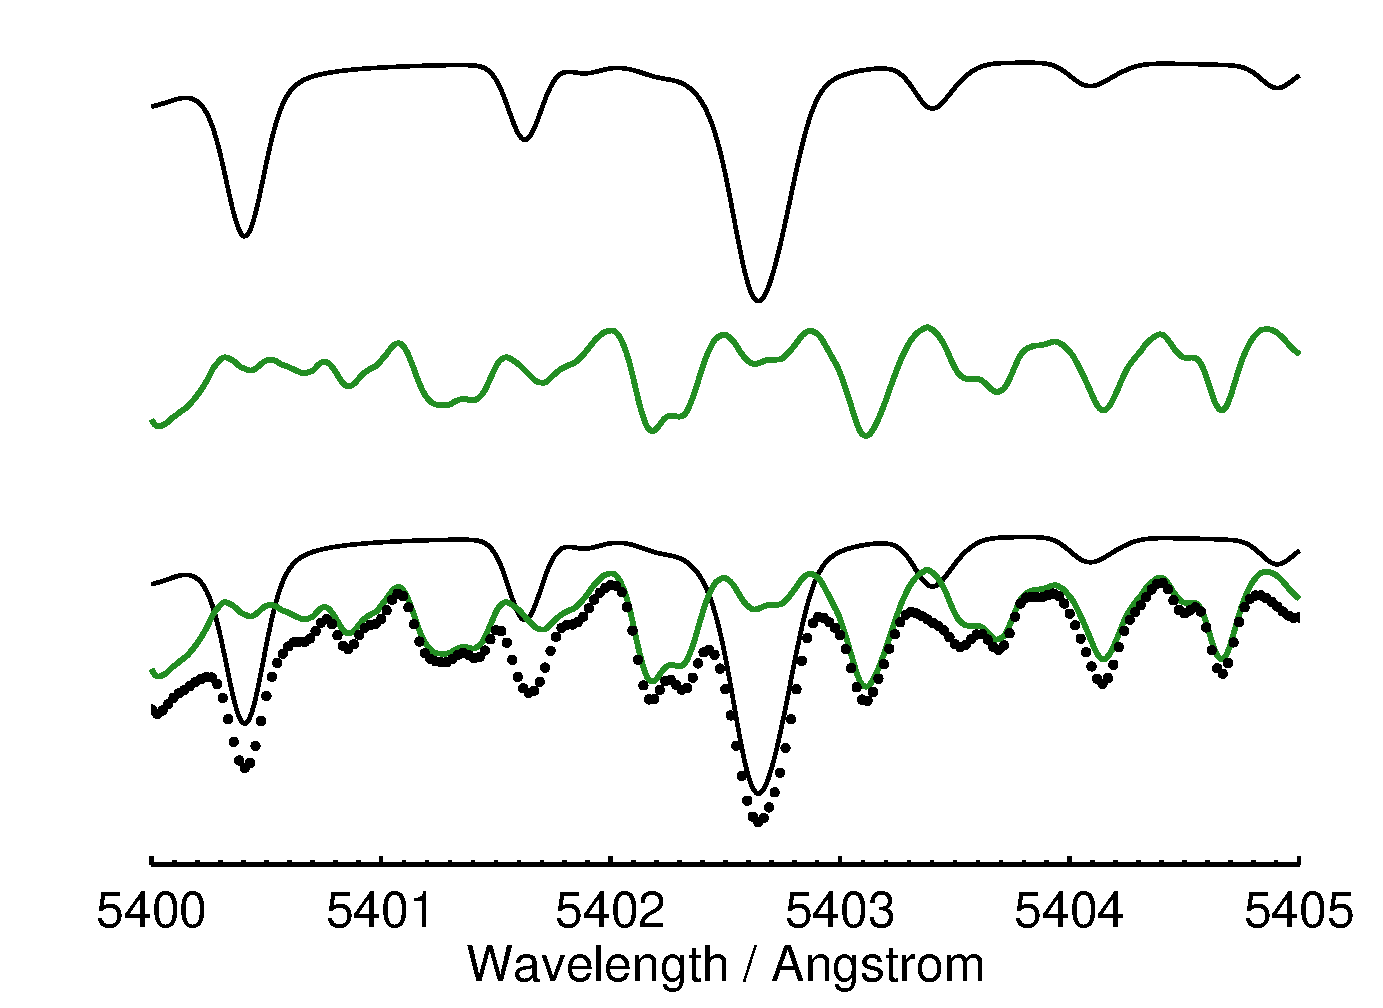
\includegraphics[scale=0.6]{doppler/forward_modeling.eps}
\caption{An illustration for the forward modeling process for
  iodine-calibrated stellar spectrum. The top black line represents
  the stellar reference spectrum (DSST), and the middle green line
  represents the iodine reference spectrum. Both reference spectra are
  convolved with an IP only for illustration purposes in order to have
  a clear match with the observed spectrum, plotted in black dots on
  the bottom. In practice, the reference spectra are multiplied {\it
    first} and then convolved with IP. \label{doppler:fig:modeling}}
\end{figure}
%----------------------------------------------------------------



%-------------------------------------------------------------------------------
\subsection{The Reference Spectra}

Ideally, the reference spectra are the ``ground truth" spectra,
i.e. the intrinsic spectra of the sources (e.g., the iodine cell, or
the star) without Doppler shift or being broadened by the
spectrometer. In reality, there is no way of knowing such ``ground
truth", so the reference spectra are empirically derived from
observations.

% how iodine atlas is made
The iodine reference spectrum, often referred to as the iodine atlas,
originates from a Fourier Transform Spectrometer scan of the iodine
cell illuminated by a continuum source. It is often of very high
signal-to-noise ratio (SNR) with high resolution (normally $\sim
500,000$ or larger). Therefore, it is generally regarded as basically
the ``ground truth" for the cell, especially for the purpose of
forward modeling lower-resolution ($\sim 60,000$) spectra. However,
there can be problems with the iodine atlas, for various reason. See
Chapter~\ref{chap:het} Section~\ref{het:sec:fts} for more on this
topic. The current FTS iodine atlas being used for \keck\ RV work is
from a scan in 1993, using the Babar FTS at NSO/KPNO, and so is the
atlas for \het. See Section~\ref{het:sec:fts} for more on iodine
reference spectra.

% how DSST is made
The stellar reference spectrum for any star, or internally to CPS
referred to as the Deconvolved Stellar Spectral Template (DSST), is
empirically derived from observed spectra of the target star. For most
of the CPS targets (bright stars), a few (4-5) observations of the
star with a narrower slit ($R \geq 80,000$) are taken without the
iodine cell in the light path. Then they are stacked together to boost
the SNR ($>500$), and then deconvolved with proper IPs derived from
bracketing B star $+$ iodine observations. The wavelength solution for
the DSST also comes from the bracketing B star $+$ iodine
observations. See Section~\ref{keck:sec:dsst} for more information and
problems related to DSSTs. For faint stars where obtaining stellar
template is expensive or unfeasible, \cite{2006ApJ...647..600J}
developed a technique where they ``morph" a synthetic stellar spectrum
or an existing DSST of another star with similar stellar properties to
fit the stellar iodine observation, and then they use this new morphed
DSST for RV extraction.


%-------------------------------------------------------------------------------
\subsection{The Functional Forms of the Instrumental Profile}\label{doppler:sec:ip}

The IP $\curlyp(x)$ can take many functional forms, and for \keck, an IP of sum of
gaussians works exceptionally well ($\chi^2 \sim 1$ for pure iodine
absorption line fit). The mathematical form for it is:
\beq
\curlyp_{\rm gaus}(x) = \sum A_n \exp{\left[\left(
    \frac{x-\mu_n}{\sigma_n} \right)^2\right]}. 
\eeq
$A_n$ stands for the amplitude for each gaussian component. $A_n$'s
are floated parameters for the fitter to optimize while $\mu_n$ and
$\sigma_n$ (i.e., positions and widths of the gaussians) have
empirically-optimized fixed values, depending on the instrument
setting of \keck\ (e.g., slit width). For \keck\ precise-RV mode (B5
decker, $\sim$60,000 resolution, with iodine cell in light path), the
IP contains 12 free parameters, $A_1, A_2, ..., A_{12}$, while $A_0$
is fixed to 1 (the big central gaussian) and $\mu_n, n=0,...,12$ and
$\sigma_n, n=0,...,12$ also have fixed values.

Another frequently used IP is the Gauss-Hermite (GH)
function, which is composed of gaussians multiplied by Hermite
polynomials $H_n$:
\beq
\curlyp_{\rm GH}(x) = \sum A_n u_n(x) = \sum A_n 
\left( \frac{2}{\pi w^2} \right)^{1/4} \frac{1}{\sqrt{n!2^2}} H_n
\left( \frac{\sqrt{2}x}{w} \right) \exp{\left[
    -\left(\frac{x}{w}\right) ^2  \right]}.
\eeq
Mathematically, any sum of gaussians can be decomposed into orthogonal
GH terms\footnote{See
  http://math.stackexchange.com/questions/28719/how-to-decompose-displaced-hermite-gauss-function-into-higher-order-hgs
  for an illustration, retrieved on March 18 2016.}, and therefore, in
principle, the GH IP should present a generic and flexible option for
IP choices. However, in reality, the least-$\chi^2$ solver is
extremely sensitive to the choices of initial guesses, even for
orthogonal bases. As a result, GH IP normally does not outperform sum
of gaussians (e.g., see work by \citealt{2013AAS...22114908V}). The GH
IP is what we use for extracting RVs from \het\ data. See
Chapter~\ref{chap:het} Section~\ref{het:sec:ip} for more.



%%%%%%%%%%%%%%%%%%%%%%%%%%%%%%%%%%%%%%%%%%%%%%%%%%%%%%%%%%%%%%%%%%%%%%%%%%%%%%
% structure of the code
\section{Code Structure and Work Flow}

This section documents the structure of the CPS Doppler code, with the
main goal to help any reader who wishes to adopt this code for their
own work. Figure~\ref{doppler:fig:flowchart} illustrates the code's
calling sequence. 


%----------------------------------------------------------------
% Figure: Code flowchart
\begin{figure}
%\epsscale{1.15}
  \centering
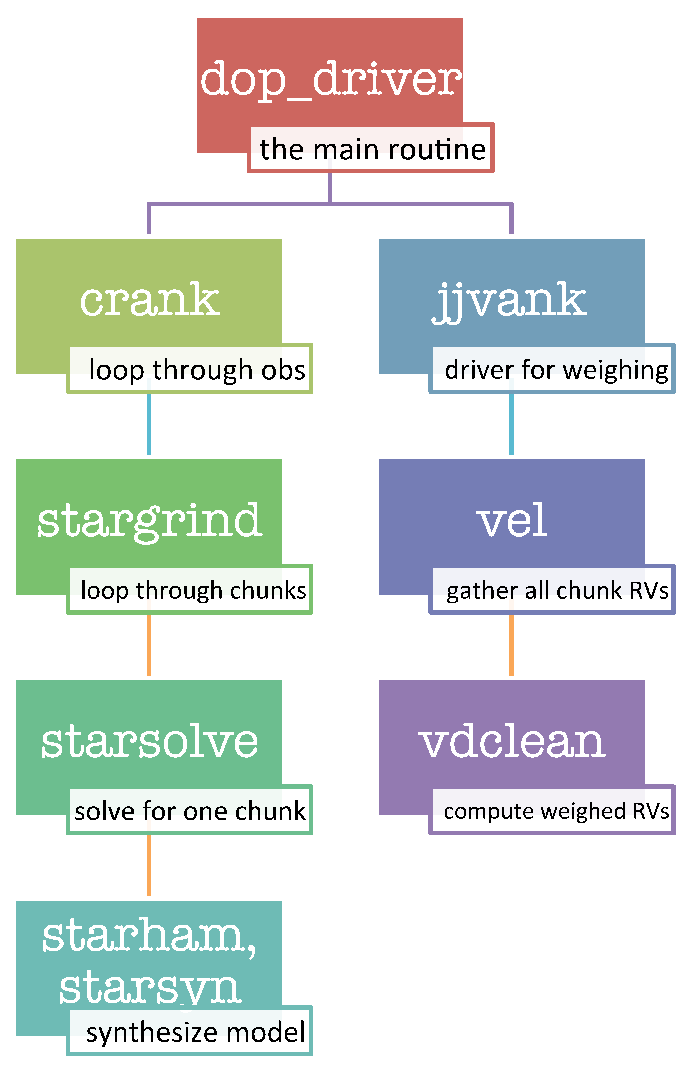
\includegraphics[scale=0.6]{doppler/flowchart.eps}
\caption{Calling sequence and main functionality for core IDL
  routines in the CPS Doppler code. \label{doppler:fig:flowchart}}
\end{figure}
%----------------------------------------------------------------


%-------------------------------------------------------------------------------
\subsection{Extracting RVs from Stellar $+$ Iodine Observations}

% dop_driver.pro and output files
The most top-level routine for running Doppler reduction is the IDL
procedure {\tt dop\_driver.pro}, which takes in the name of the star
and then automatically locate input files such as the extracted 1-D
spectra, the proper DSST file, the iodine atlas, and the files storing
initial guesses for parameters (which are called the {\tt vdiod}
files). The code is also very flexible with inputs and the user can
specify almost anything, e.g., a specific DSST file, choice for a
specific IP model, explicit initial guesses for parameters, and so
on. It drives the Doppler analysis and output a {\tt vd} file for each
observed spectrum, which contains best-fit parameters and other
information for all the spectral chunks. At the end, {\tt
  dop\_driver.pro} calls {\tt jjvank.pro}, which combines the RVs from
all the chunks in all the observations for this star, and evaluates
numerical weights for each chunk and each observation. Finally, {\tt
  jjvank.pro} computes the weighted RV for each observation and its RV
uncertainty and outputs the information in {\tt vst} files. The most
useful variable is the {\tt cf3} structure in the {\tt vst} file,
which contains, for example, the Julian Date (JD) of the observation
{\tt cf3.jd}, the BC {\tt cf3.bc}, the weighted RV {\tt cf3.mnvel},
and its uncertainty {tt cf3.errvel}. The algorithm for {\tt
  jjvank.pro}, or ``vanking", is described in the next
subsection. In the end, {\tt dop\_driver.pro} will produce $N_{\rm obs}$
{\tt vd} files and one {\tt vst} file for each star. If a new
observation is taken, a new {\tt vd} file is created, and vanking
re-evaluates the chunk and observation weights and outputs a new {\tt
  vst} file.

% crank.pro and the three passes
While {\tt dop\_driver.pro} is the routine to call for Doppler
analysis, most of its actual codes simply deal with logistical work
such as locating the right files. The real driver behind the scene is
{\tt crank.pro}, which contains the loop through all observations and
``fills out" the {\tt vd} files. In a standard CPS reduction routine,
{\tt crank.pro} is called three times. In the case of \keck\ standard
RV reduction, for example, the first time {\tt crank.pro} is called,
it fits for all 15 free parameters ($z$, $w_0$, $w_d$ and 12 IP
parameters; see Table~\ref{doppler:tab:rvpar}) for each chunk in each
observation. The LM fitter takes in the initial guesses for parameters
from B star $+$ iodine solutions and tries its best to optimize the 15-parameter
model. Due to the complexity of this multi-modal and multi-dimensional
problem, very often the best fit for this ``first pass" does not yield
a good global minimum on the $\chi^2$ surface. Therefore a second
pass of {\tt crank.pro} is called, with fixed IP parameters and thus
only three free parameters. The IP parameters are not simply fixed to last
round's best-fit values, but instead, they were fixed to describe an
``averaged" IP over a region on the CCD chip (for example, over a
neighbor of nine chunks across three spectral orders for the central
chunk). After the second pass, a third pass of {\tt crank.pro} is
called with fixed wavelength dispersion $w_d$ and only floating $z$
and $w_0$, in search for a deeper minimum or lower $\chi^2$.

% other layers inside crank.pro
Within {\tt crank.pro}, the code calls for {\tt stargrind.pro} in a
loop of all observations. {\tt stargrind.pro} does the model fitting
for a single observation, and it loops through all spectral chunks,
calling {\tt starsolve.pro}, which contains the LM fitter, for each
chunk. Inside {\tt starsolve.pro}, the spectral model is computed
using {\tt starham.pro}, which is really just a wrapper around {\tt
  starsyn.pro}. The core algorithm for model construction is all in
{\tt starsyn.pro}, which takes in the observed 1-D spectral chunk, the
DSST, the iodine atlas, and the model parameters, and outputs a model
spectrum for this chunk. 



%-------------------------------------------------------------------------------
\subsection{Computing Weighted Average RVs for Each Observation}

Now all observations and all chunks have their best-fit model parameters
computed by {\tt crank.pro}, and all RVs are barycentric
corrected. What's next?

Two extremely important things need to happen at this point before we
can have an RV time series in hand, and they are accomplished by {\tt
  jjvank.pro} and most importantly, {\tt vdclean.pro} (see
Figure~\ref{doppler:fig:flowchart} for the calling sequence).

% need to adjust chunk zero point
First, the chunk RVs need to be adjusted so that they have the same
``zero point". As mentioned in the previous subsection, the measured
RV for each chunk at a certain epoch $T_{\rm obs}$ is a relative RV
against the DSST taken at epoch $T_0$, $v_{*,\T_{\rm obs}} -
v_{*,T_0}$. This is because the stellar lines and their Doppler shift
in each chunk are modeled by red-shifting the DSST: $F_{*}'(\lambda) =
F_{*}(\lambda\cdot(1+z))$. The wavelength solution for the DSST
implies its absolute RV $v_{*,\ T_0}$ at $T_0$. If the wavelength
solution for all DSST chunks corresponds to the exact same value of
$v_{*,\ T_0}$, then measured RVs for all chunks in the observed
stellar iodine observation would have the same ``zero
point". Consequently, any biases or relative errors in the DSST
wavelength solution would result in a shifted zero point for that
chunk with respect to other chunks. For example, one source of error
comes from the fact that the wavelength solution for DSST is derived
from neighboring B star $+$ iodine observations, which assumes that
the wavelength solution for the orders and pixels remain the same
between the B star and the DSST observations. Or, the wavelength
solution derived from B star observations may be imperfect.

There also could be other reasons why the RV zero point of a chunk
deviates from the other chunks. Things like CCD effect, errors in
iodine atlas or DSST, 
zzz other sources for zero point shifts. The scatter in RV zero points
will translate  

% need to compute weights for each chunk and observation
Second, 

% the algorithm

\chapter{Improving the Radial Velocity Precision of HET/HRS}\label{chap:het}


%%%%%%%%%%%%%%%%%%%%%%%%%%%%%%%%%%%%%%%%%%%%%%%%%%%%%%%%%%%%%%%%%%%%%%%%%%%%%%
\section{Introduction and Background}

This is about HET/HRS. This will have introduction to HET and HRS.

make sure to mention set up of slit in front of the fiber.

Motivation behinding using HRS, including its advantages, such as
queque schedule and fiber feed. However, it never performed on 1-2~m/s
level in terms of RV precision like \keck.

Temperature stability in the spectrograph room of \hrs\ was identified
early on as one of the contributing factors to the RV systematic
errors, and this issue was resolved since the installation of a fine
temperature control system in March 2008 (J.~Bean, L.~Ramsey,
P.~McQueen private communications). The temperature fluctuation is now
controlled down to $\ll$1~K from 10~K. We confirmed the improvement in RV
precision as a result of this upgrade in our analysis with the HD
37605 data, which is illustrated in the lower panel of
Figure~\ref{het:fig:tempstable}. The RMS of \hrs\ velocities with
respect to the best Keplerian fit of the HD 37605 system is 9 m/s for
data before March 2008, and it is reduced to 6 m/s for data
afterwards. Such improvement is encouraging, and a closer look at the
data and the intermediate products of the Doppler pipeline reveals
even more potential contributors to the RV instability of \hrs, which
is the theme of this chapter.


%----------------------------------------------------------------
% HD 37605 and the improvement on precision brought by temperature stabilization
% plot made by ~/ExoPlanet-2010-2011/Targets/37605/rv_plot/rvplot_NESSF2013.eps
% grabbed from ~/ExoPlanet-2010-2011/Professional_Development/201301-NESSF/proposal/
\begin{figure}
\centering
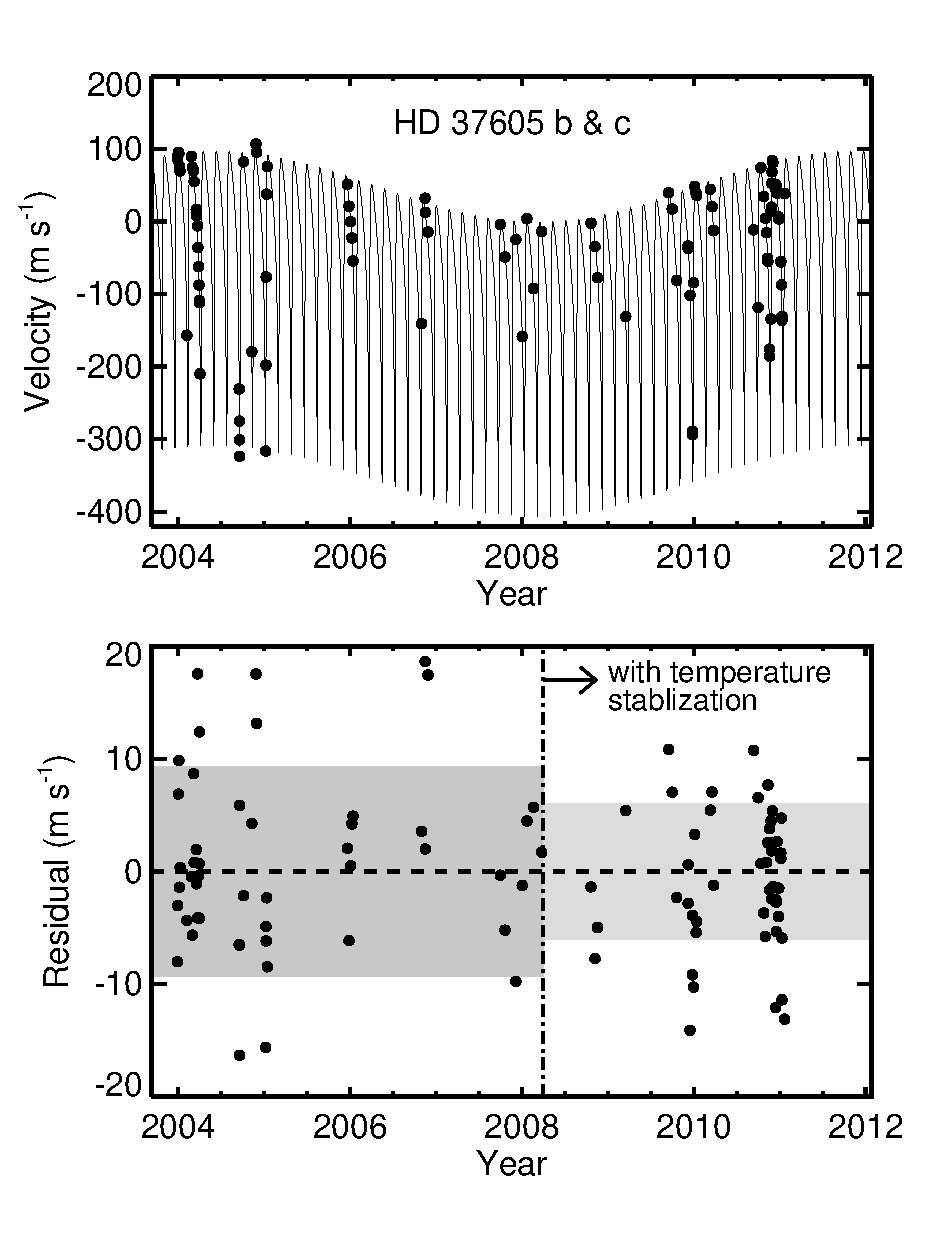
\includegraphics[scale=0.5]{het/37605.eps}
\caption{Illustration of the effects of temperature stabilization on
  \het\ RV precision, using data on the HD~37605 system (see
  Chapter~\ref{chap:planets}). The RMS of the RV residuals (bottom
  panel) against the best-fit two-planet Keplerian solution (solid
  line in top panel) has dropped from 9~m/s to 6~m/s (grey areas in
  the bottom plot) after implementation of fine temperature control in
  the spectrograph room in March 2008. The pre-2009 \het\ data are
  provided by the UT Austin group.
\label{het:fig:tempstable}}
\end{figure}
%----------------------------------------------------------------


We set out to first construct a data reduction and RV extraction
pipeline for \het, which is described in
Section~\ref{het:sec:pipeline}. Then we tried to improve the precision
by seeking out for a better instrumental profile (IP) model, i.e., a
functional form that can bring good fit to \het\ data, which is
documented in Section~\ref{het:sec:ip}. Section~\ref{het:sec:fts}
describes our efforts in validating the iodine cell Fourier Transform
Spectrometer (FTS) scans for \het\ and our investigation on the
plausible changes in cell properties.


%%%%%%%%%%%%%%%%%%%%%%%%%%%%%%%%%%%%%%%%%%%%%%%%%%%%%%%%%%%%%%%%%%%%%%%%%%%%%%
\section{Adoption of REDUCE and the CPS Doppler Code for
  HET/HRS}\label{het:sec:pipeline} 

We built a data reduction pipeline for \het\ that performs automatic
raw spectral data reduction and RV extraction for any target star or
HET observing program.

The first part of our data pipeline is the raw reduction code, which
reduces the raw spectral images with calibration frames and produces
FITS files containing the extracted 1-D spectrum for each spectral
order.  We adopted the REDUCE reduction package by
\cite{2002A&A...385.1095P}. Sarah Gettel and Steve Bongiorno did the
initial adoption of the REDUCE package for reducing \het\ data. It
involved much parameter tuning with the original package to make this
optimal extraction code, which was designed for slit-fed spectrometer
like \keck\ and Lick/Hamilton, to work with the fiber-fed HRS data.
The most important modification we did was to automate the routine for
tracing the echelle orders on the spectral image, which used to
require human-intervention (i.e., clicking on the echelle orders to
help the code recognize the traces). Capitalize on the fact that the
shape of the order traces do not change significantly across time, we
use a set of previously fit polynomials that describe the trace
positions and shift them to match the traces on the raw image via
cross correlation. We also wrote wrapper routines to automate patch
reduction for \het\ observation programs or any single target star.

The second part of our data pipeline is the code that extracts RVs
from the 1-D spectral data. We adopted the CPS Doppler code, which is
documented in Chapter~\ref{chap:doppler}. The adoption process mostly
involved bookkeeping and code debugging works to make sure it could
run on Penn State Astronomy network machines, to train
the code to recognize \het\ images, to work with our local file
structures, and to be able to produce DSST locally using \het\ data
(instead of using \keck\ DSST like we did initially, which does not
produce RVs as precise as using \het\ DSSTs). 

In the spirit of making it easier for any future CPS code adopters, we
document the requirements and procedures for making such an adoption
below. Many of these procedures would not make sense to someone who
has not handled the CPS Doppler code before, but they are tremendously
time-saving for anyone who wants to use the CPS code to extract RVs
from their own spectra.\\

{\bf Required files for Doppler reduction:}
\begin{itemize}
\item Reduced, extracted 1-D spectra with both iodine and stellar
  lines. The 2-D matrix holding the 1-D spectra in each order should
  have the format {\tt matrix[pixel, order]}.
\item A log file which lists: observation ID, target of the
  observation, JD, barycentric velocity correction for the target for
  the observation, and nature of the observation (iodine cell in light
  path?). The default log file should be in the {\tt /bary/} folder but
  it can be customized via keywords of {\tt dop\_driver.pro}.
\item A {\tt vd} example file (an IDL save file) which contains an
  example {\tt vd} structure for the spectrograph. The {\tt vd}
  structure also contains definition for spectral chunks, i.e.\ their
  orders and starting and ending pixels. It also contains first guesses
  for the parameters for each chunk (most importantly, a rough
  wavelength solution which must be good within 20 pixels). This should
  be in the {\tt /files/} folder.
\item An IPGUESS file (IDL save file) with the structure {\tt
    ipguess}, which contains the JD and file names for the {\tt vd} files
  to be used as first guesses of parameters. The {\tt ipguess} structure
  must contain at least one {\tt vd} file entry, and very often it has
  many entries so that the code can pick the most recent one. This
  should be in the same folder as the Doppler code.
\item A DSST file (IDL save file) with the {\tt DSST} structure, which
  contains the DSST spectrum in chunks, and the definition of chunks
  must be consistent with the example {\tt vd} structure. This should be
  in the {\tt /files/} folder.
\end{itemize}

{\bf List of routines to modify:}
\begin{itemize}
\item {\tt dop\_driver.pro}
  \begin{itemize}
    \item Add a keyword to distinguish runs for your instrument, e.g.,
      ``het=het'' for \het\ reductions.
    \item Add codes to define necessary data paths near line 124.
    \item Add a line near line 406 so that the code recognize the
      first two characters in your observation name, which will be used as
      an identifier for your instrument. For example, the \het\ observations
      are named as ``20160101.00001'', so the identifier for \het\ data is
      ``20'' (it is ``rj'' for post-detector upgrade \keck\ data).
    \item If you want the sum of Gaussians IP for your instrument,
      add this option near line 75.
  \end{itemize}
\item {\tt crank.pro} Near line 164, add instrument setups such as
  data paths.
\item {\tt rdsi.pro} Add option ({\tt tp eq '20'} for \het) for
  reading in the spectral data for your instrument.
\item {\tt chip.pro} Add gain value for your detector, even if your
  reduced spectra are gain-corrected already (then just have {\tt gain =
    1}).
\item {\tt vdcube.pro} Define the {\tt highcts} near line 120 for your
  detector, which defines the saturation threshold for your CCD and such
  observations will be disregarded during vanking. Also add your
  customized {\tt /files/} path in the code near line 168.
\item {\tt rdhbcvel.pro} At the beginning, make sure this code knows
  that it is handling data specific to your instrument (using, for
  example, the name of your log file as identifier). Then near line 80,
  you want to define a full file name for your reduced 1-D spectra based
  on the observation ID.
\item Making your own DSST? {\tt
    /rv/deconv/deconvolve\_stellar\_template.pro} contains the code to
  make DSST using \het\ data. A quick walk through {\tt
    make\_dsst\_keck\_psu.pro} and compare it with {\tt make\_dsst.pro}
  will also tell you how to modify {\tt make\_dsst.pro} to make it work
  for your template observations.
\end{itemize}

There could be other ad hoc places that need to be modified to
accommodate your customized 1-D spectrum format. For example, around
line 523 in {\tt stargrind.pro}, the code defines a lower boundary for
wavelength at 5000\AA, which is completely arbitrary, and the user may
need to modify this to accommodate any orders bluer than 5000\AA. Or,
if you are using sum of Gaussians as your IP model, you want to modify
{\tt getpsf.pro} for customized positions and widths for your
satellite Gaussians.

A typical call to run the Doppler code looks like this:\\
{\tt
  dop\_driver,'target.star.name','your.short.tag',dsstname='file name
  of your DSST',\\
dsstobnm='observation name of your DSST',/gh,/vank,/noprint,/het, \\
tag='your.long.tag'
} \\ 
The previous chapter is a general documentation of how the CPS Doppler
code works. Other useful documentation for the code are in the {\tt /doc/}
folder.

After we completed our data pipeline, we immediately reduced the data
on HD 185144, which is a favorite RV standard at both Keck and HET and
also many other precise RV facilities. The results, plotted in
Figure~\ref{het:fig:sigdra}, were very encouraging -- a 3-4 m/s
precision {\em out of the box}, without any tuning of the Doppler
code. It is also found out later that the RVs produced using the \het\
DSST are better than the ones with \keck\ DSST, possibly because the
errors in the deconvolution and the forward modeling (convolution)
would cancel out if the DSST and star$+$iodine data come from the same
telescope, which is a folklore among the iodine precise RV artists.

%----------------------------------------------------------------
% HET sig dra RV data, Keck DSST vs. HET DSST
% plot made by ~/Ex../Professional.../201305-HET_propo../plots/*.pro
% and saved therein
\begin{figure}
\centering
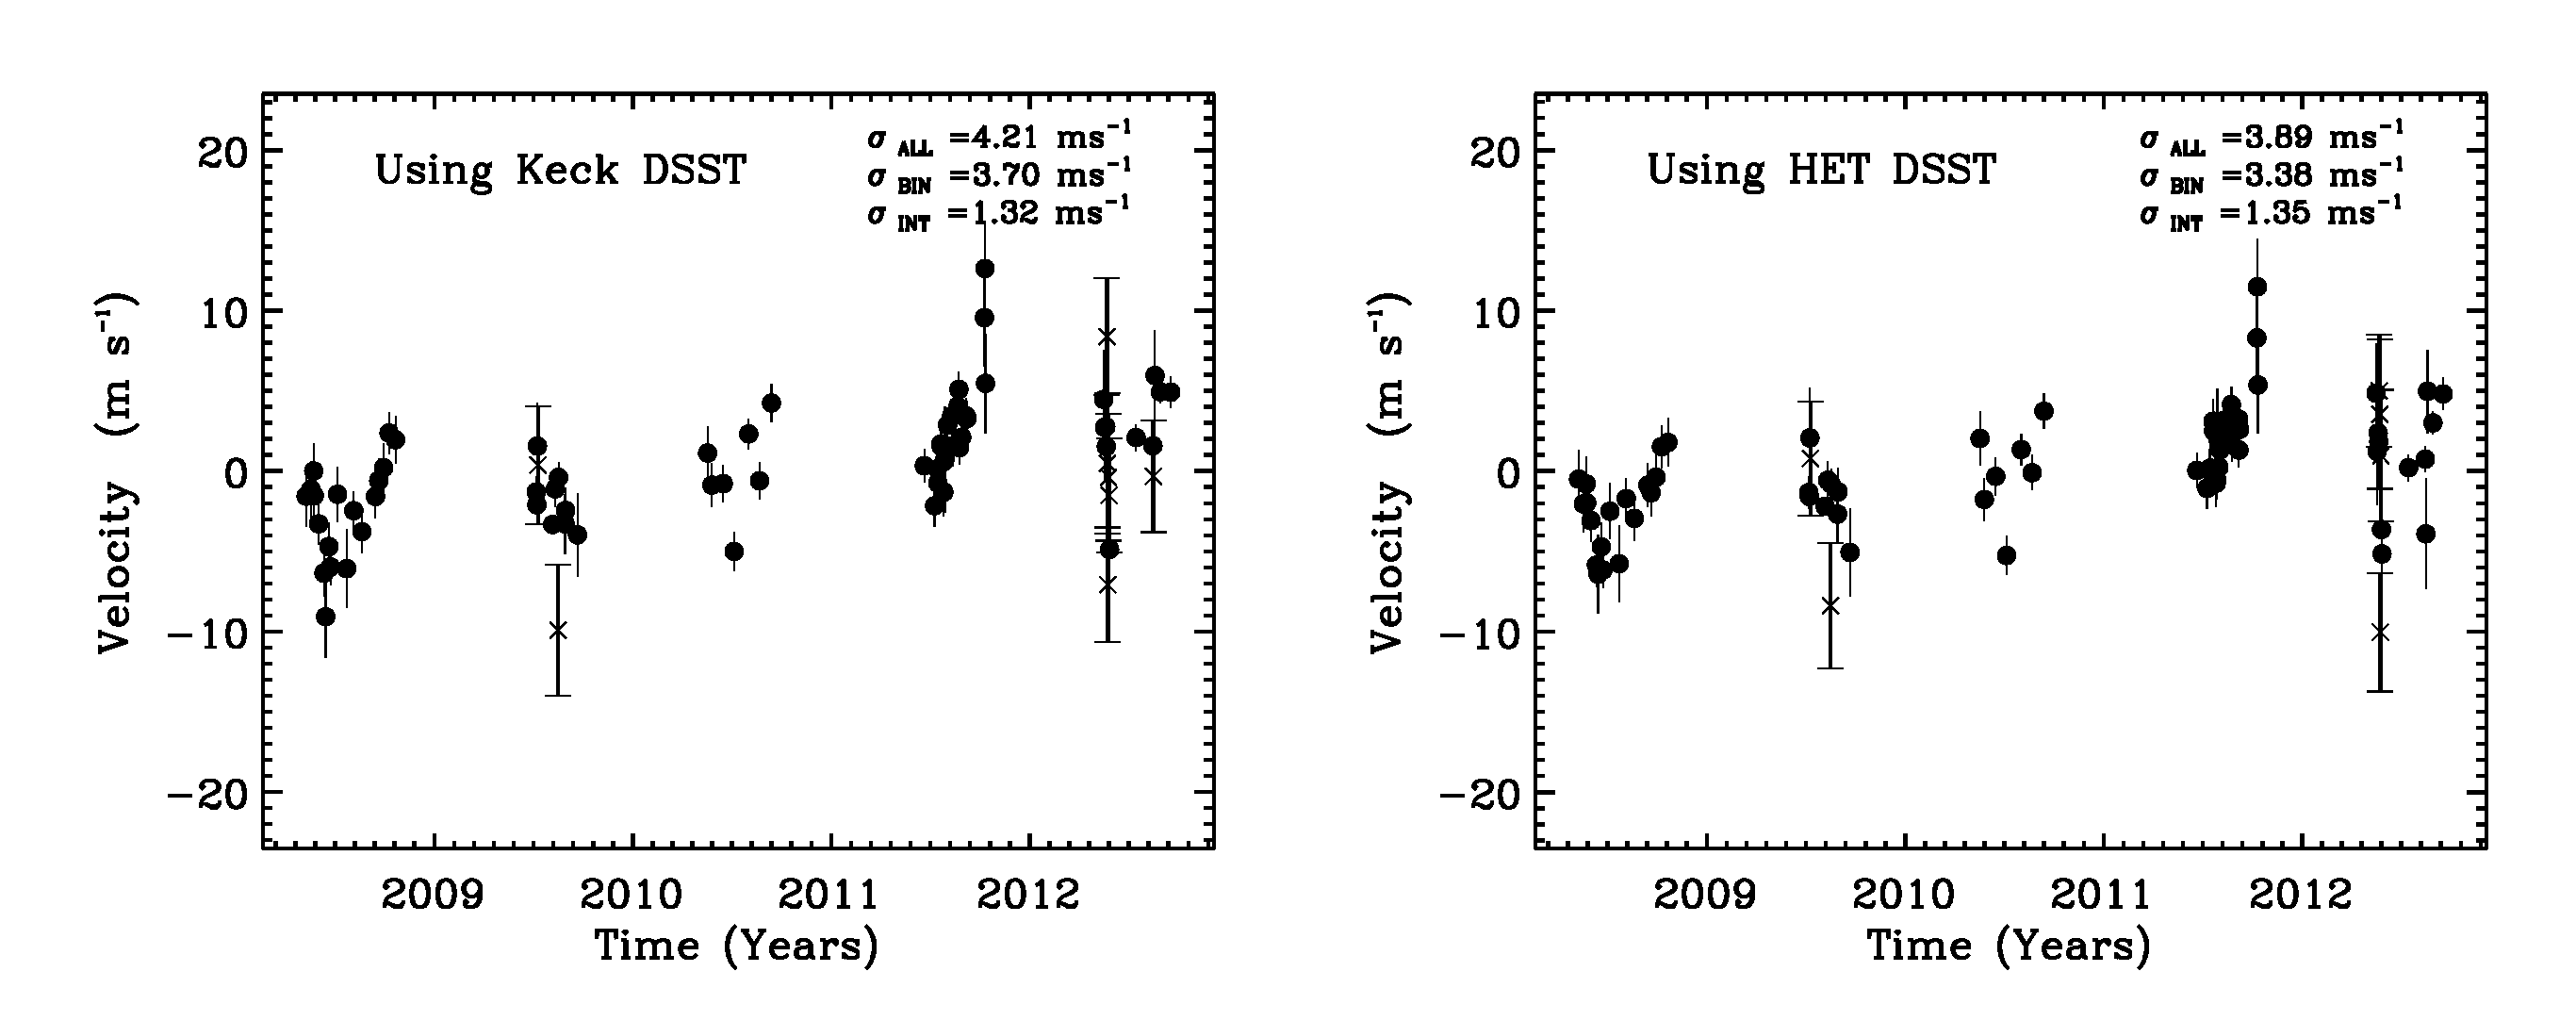
\includegraphics[scale=0.3]{het/sigdra.eps}
\caption{RV time series on HD 185144 as observed by \het\ and reduced
  by our data pipeline. The left panel shows RVs extracted using the
  Keck HD 185144 DSST, and the right panel shows RVs with DSST derived
  using \het\ data and the CPS code we adopted.
\label{het:fig:sigdra}}
\end{figure}
%----------------------------------------------------------------

The typical \keck\ RV RMS on HD 185144 is about 2.57~m/s. Our mission
is to find out if and how we can bring the RV precision of \het\ to
the level of \keck.


%%%%%%%%%%%%%%%%%%%%%%%%%%%%%%%%%%%%%%%%%%%%%%%%%%%%%%%%%%%%%%%%%%%%%%%%%%%%%%
\section{The Search for a Better Instrumental Profile}\label{het:sec:ip}

% HET IP section

Finding a good customized function for the instrumental profile (IP)
for a precise RV spectrograph is undoubtedly one of the most important
and difficult tasks in achieving a $<3$~m/s RV precision. IP modeling
is a crucial part of the precise RV work with iodine calibration, as
it affects directly several key procedures in the Doppler pipeline,
such as the creation of stellar spectrum template and the
forward-modeling of the observed stellar$+$iodine spectrum. The heroic
efforts of early \keck\ users pinned down its IP to a 12-parameter
sum-of-Gaussians profile, with two sets of 11 pre-determined positions
and width of the satellite Gaussians \citep{1995PASP..107..966V}. It
is the product of careful studies and numerous trials with IP
modeling.

It is very easy to imagine that imprecise and inaccurate IP modeling
could be the bottleneck for improving \het's RV precision. The ability
to capture the shape of the IP and {\em its changes} largely determines
how well the RV spectra are fitted, and thus how precisely the Doppler
shift is measured. The 3-4~m/s precision on HD 185144 we obtained
(Figure~\ref{het:fig:sigdra}) was the results of an ``out of the box''
reduction -- we had only modified the CPS Doppler code to the point
where it could process \het\ data, but we had not yet put in any
efforts to tune it for \het. The first step of such tuning would be to
find a better IP.


%----------------------------------------------------------------
% Demonstration of convolution to fit iodine atlas
% plot made by ~/Exo.../HET.../plots_general/convol_kernel/deconv_plot.pro
\begin{figure}
\centering
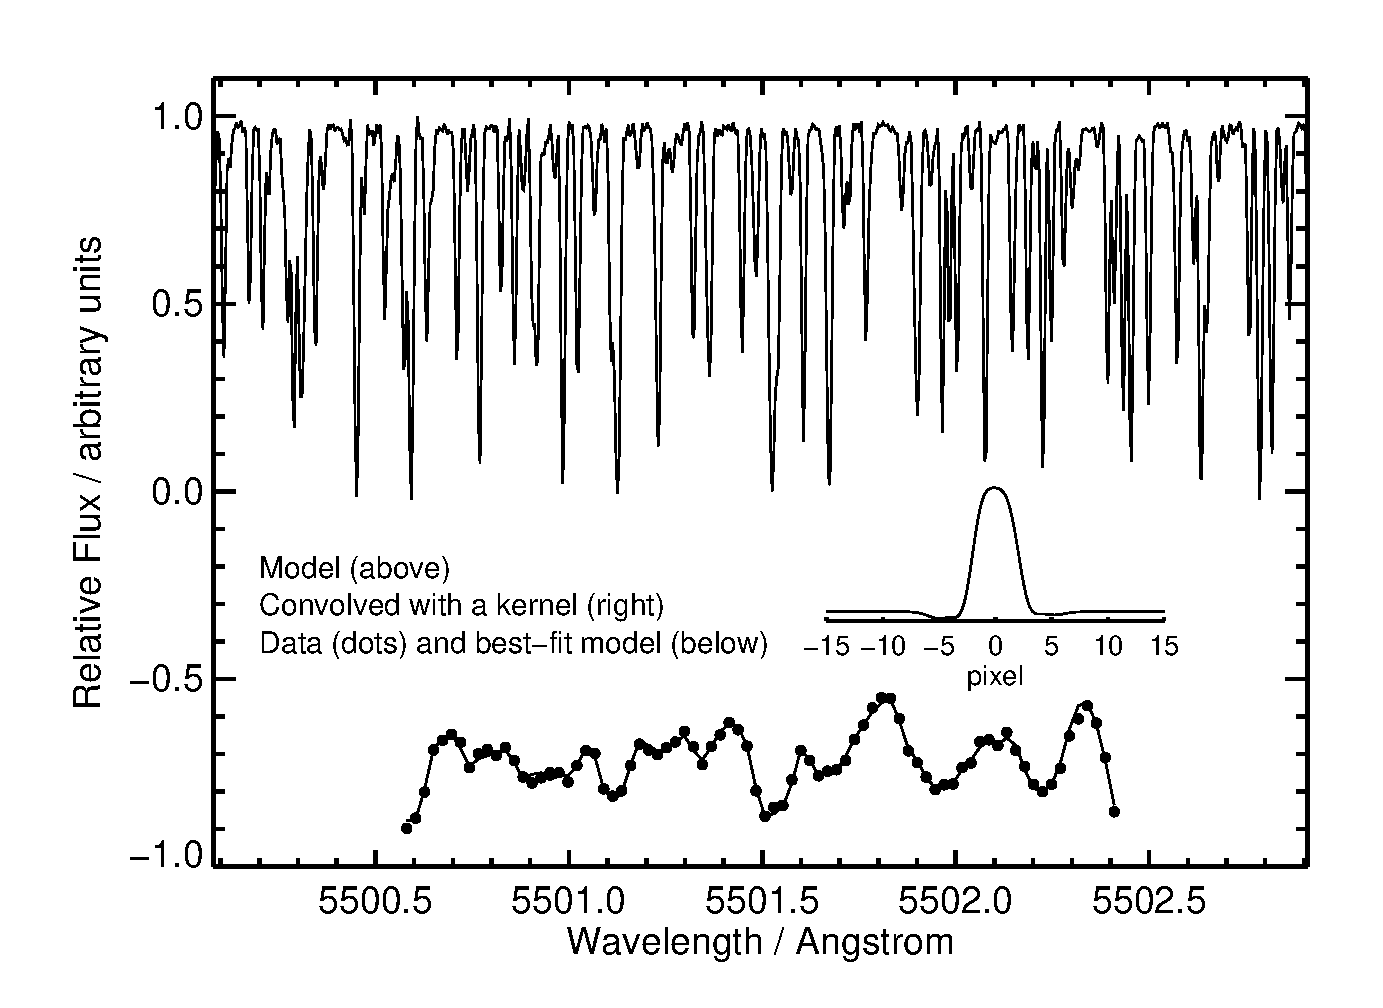
\includegraphics[scale=0.45]{het/convolution_kernel.eps}
\caption{Illustration of convolving the iodine atlas (sharp solid
  lines) with a kernel (middle right insert) to fit the observed
  iodine lines (black dots near the bottom, with best-fit model
  plotted in solid line).
\label{het:fig:convkernel}}
\end{figure}
%----------------------------------------------------------------


How well the IP is being modeled can be tested by fitting a pure
iodine spectrum taken by the spectrograph
(Figure~\ref{het:fig:convkernel}), with the continuum source being
either a lamp or a (mostly) line-free B star. Such spectra are often
referred to as the iodine spectra (or frames or flats), or the B star
iodine spectra. The typical $\chi_\nu^2$ value that we obtain for
fitting \het\ iodine spectra with a generic IP model (Gauss-Hermite
polynomials) is about 2-5, while for Keck/HIRES, the \chisq\ value is
typically around 1 (Figure~\ref{het:fig:iodchunkcomp}). The origin of
this difference in \chisq\ does not seem to rise from a
signal-to-noise difference in the spectra
(Figure~\ref{het:fig:checksnr}).


%----------------------------------------------------------------
% Comparison between HET and Keck chunk fit
% plot made by ~/Exo.../HET.../plots_general/fit_demo/plotfit.pro
\begin{figure}
\centering
\subfloat[\het\ Chunk]{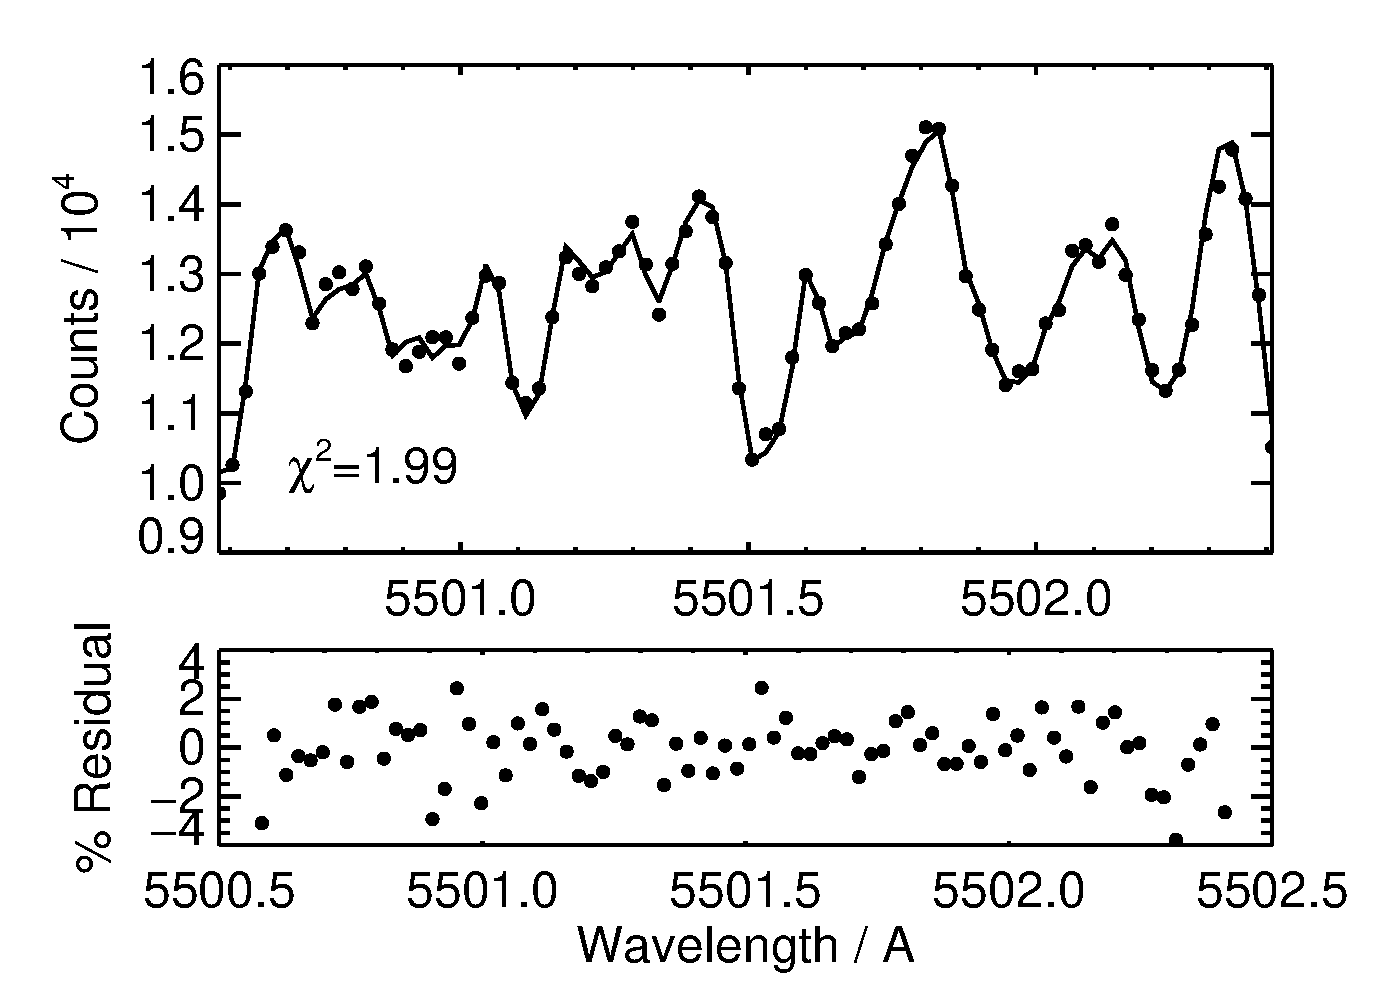
\includegraphics[scale=0.35]{het/20120124.176005.chunk189.eps}}
\subfloat[\keck\ Chunk]{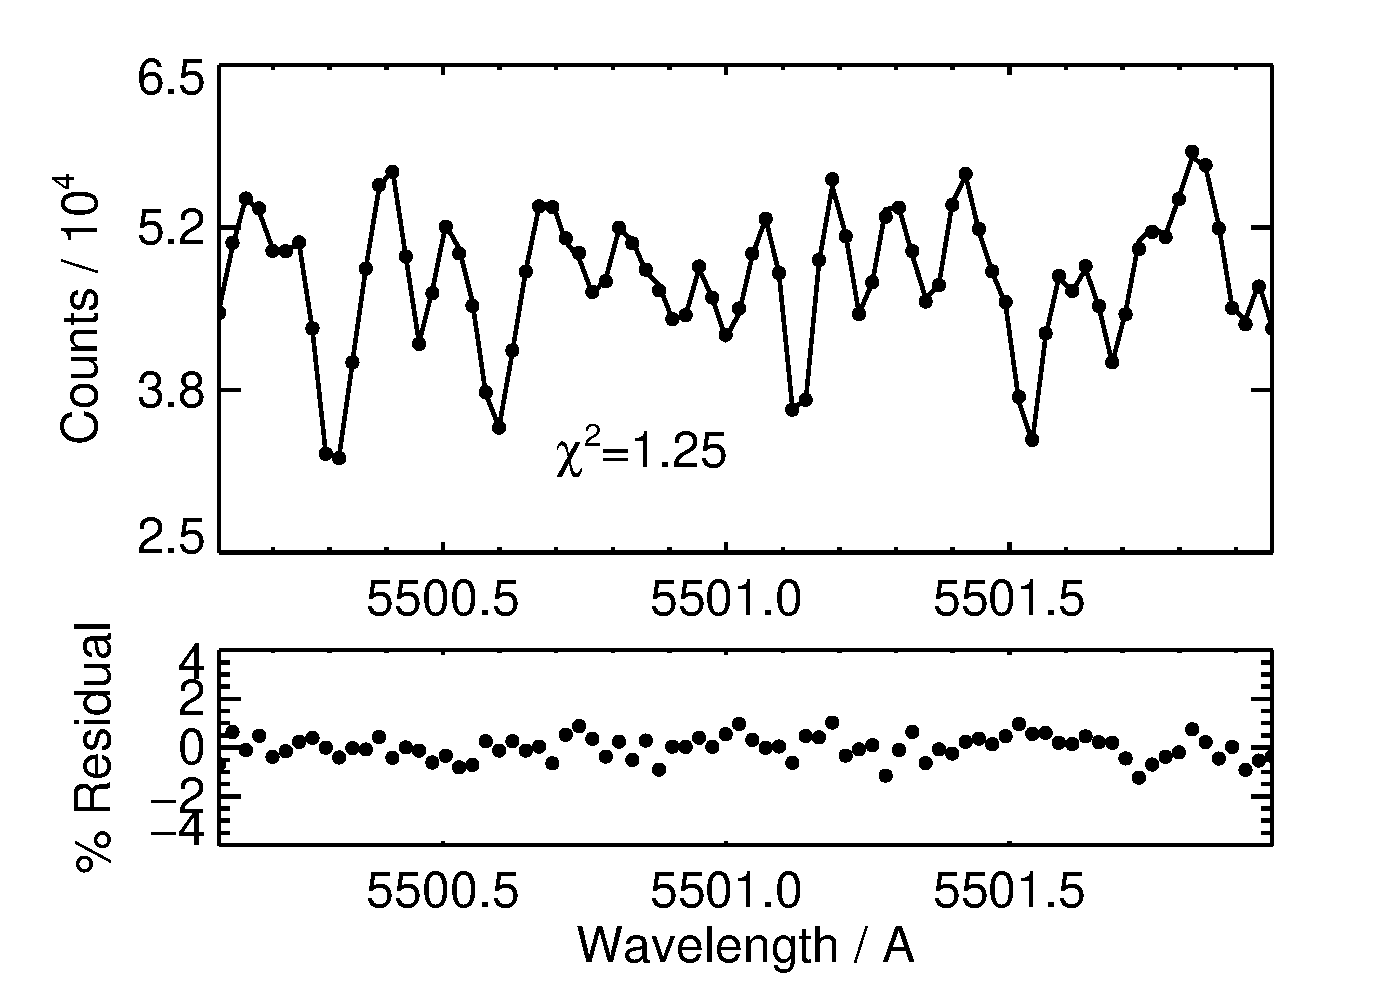
\includegraphics[scale=0.35]{het/rj82.77.chunk308.eps}}
\caption{Comparison between fits for a typical iodine-only chunk using
  \het\ data (left panel) and \keck\ data (right panel). Bottom panels
  are showing the residuals against best-fit models, plotted on the
  same $y$-axis scale. \het\ fit is significantly worse than \keck,
  which we believe is one of the major drivers behind \het's poorer RV
  precision. 
\label{het:fig:iodchunkcomp}}
\end{figure}
%----------------------------------------------------------------



%----------------------------------------------------------------
% HET and Keck chunk SNR and fit comparison
% plot made by
% ~/ExoPlanet-2010-2011/HET-HRS-IP/05-Iodine_FTS_investigation/check_snr.pro and saved in ./plots/a
\begin{figure}
\centering
\subfloat{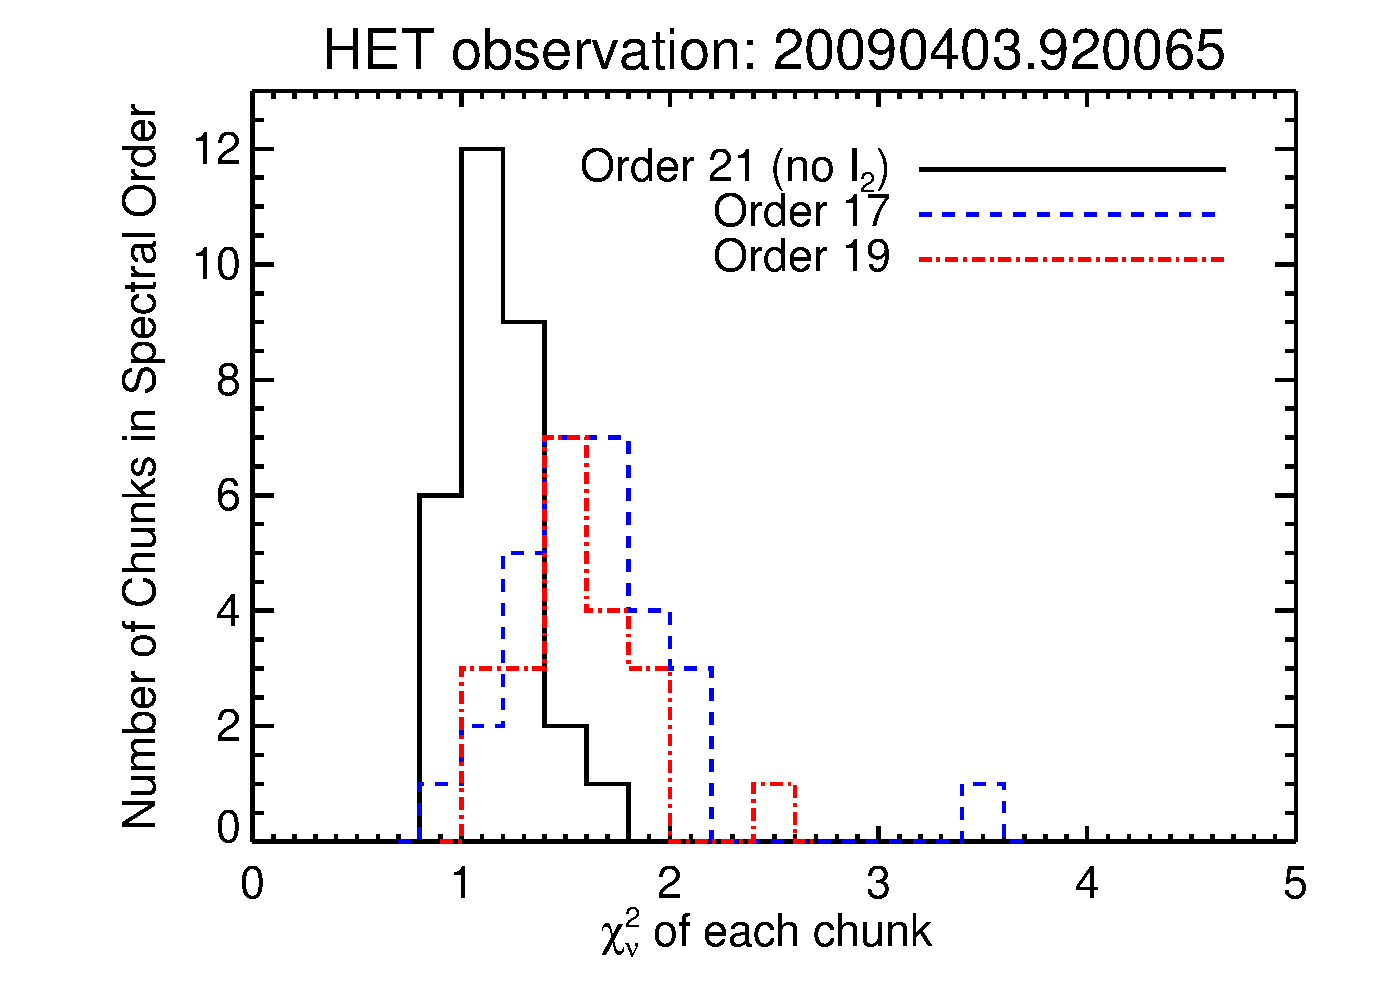
\includegraphics[scale=0.3]{het/het_check_snr.eps}}
\subfloat{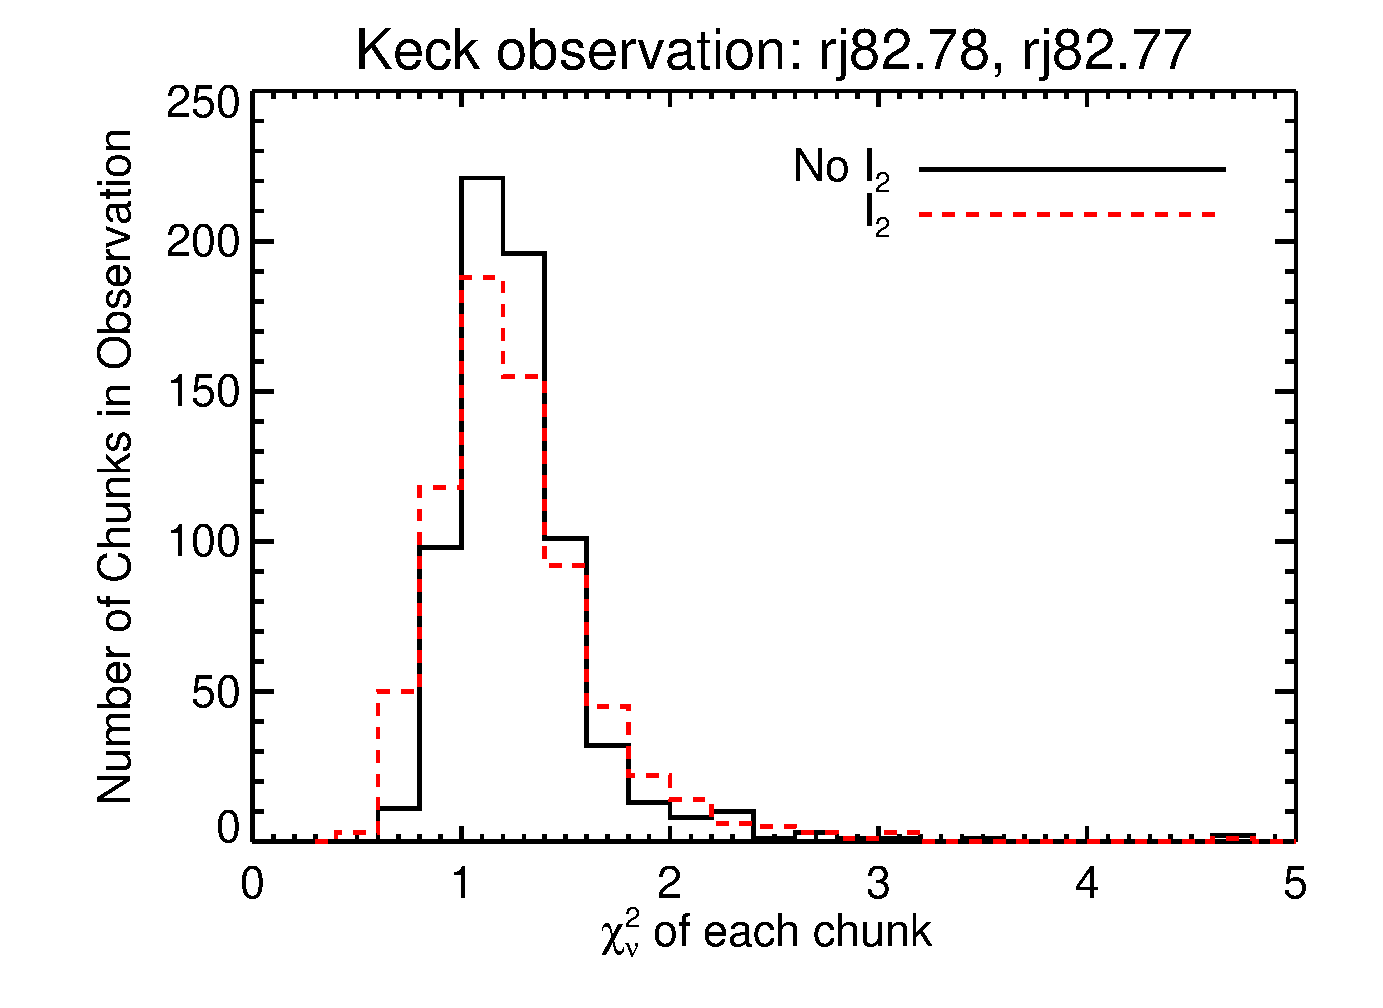
\includegraphics[scale=0.3]{het/keck_check_snr.eps}}
\caption{Comparison of fits for iodine-free region/observation
  (fitting a straight line for each chunk) and for iodine
  region/chunks. The left panel is for \het\ data in one observation,
  but using spectral orders with or without iodine lines. The right
  panel is for \keck\ data in two different observations with and
  without iodine cell in place. The fits for iodine-free spectral
  chunks turn out to be consistent what is expected with photon noise
  for both \het\ and \keck. This eliminates additional noise as a
  suspect in contributing to the bad fits to \het\ iodine spectra.
\label{het:fig:checksnr}}
\end{figure}
%----------------------------------------------------------------



The current ``go-to'' IP model for \hrs\ is the very versatile,
orthogonal, 11-parameter Gauss-Hermite polynomial (GH), which was
described in Chapter~\ref{chap:doppler}. Another customized IP for
\het\ was tried out by CPS using the sum of Gaussians, the same as
the one used for \keck\ but having the wings at different locations
with different default widths. The two IPs basically perform at a
similar level, with GH being slightly better
(Figure~\ref{het:fig:ghgau}). We have also tried several other
functional forms such as GH convolved with a top hat function with a
varying or fixed width, Lorentzian-Hermite (replacing the Gaussian in
GH with a Lorentzian), which all performed marginally worse than GH,
just like the sum of Gaussians. Or, more precisely, these IPs all seem
to be ``equally bad''.


%----------------------------------------------------------------
% Comparing 2005 and 2008 data, with GH and Gaussian IPs
% plot from ~/ExoPlanet-2010-2011/Professional_Development/201000-NSF_Jason/plots/
\begin{figure}
\centering
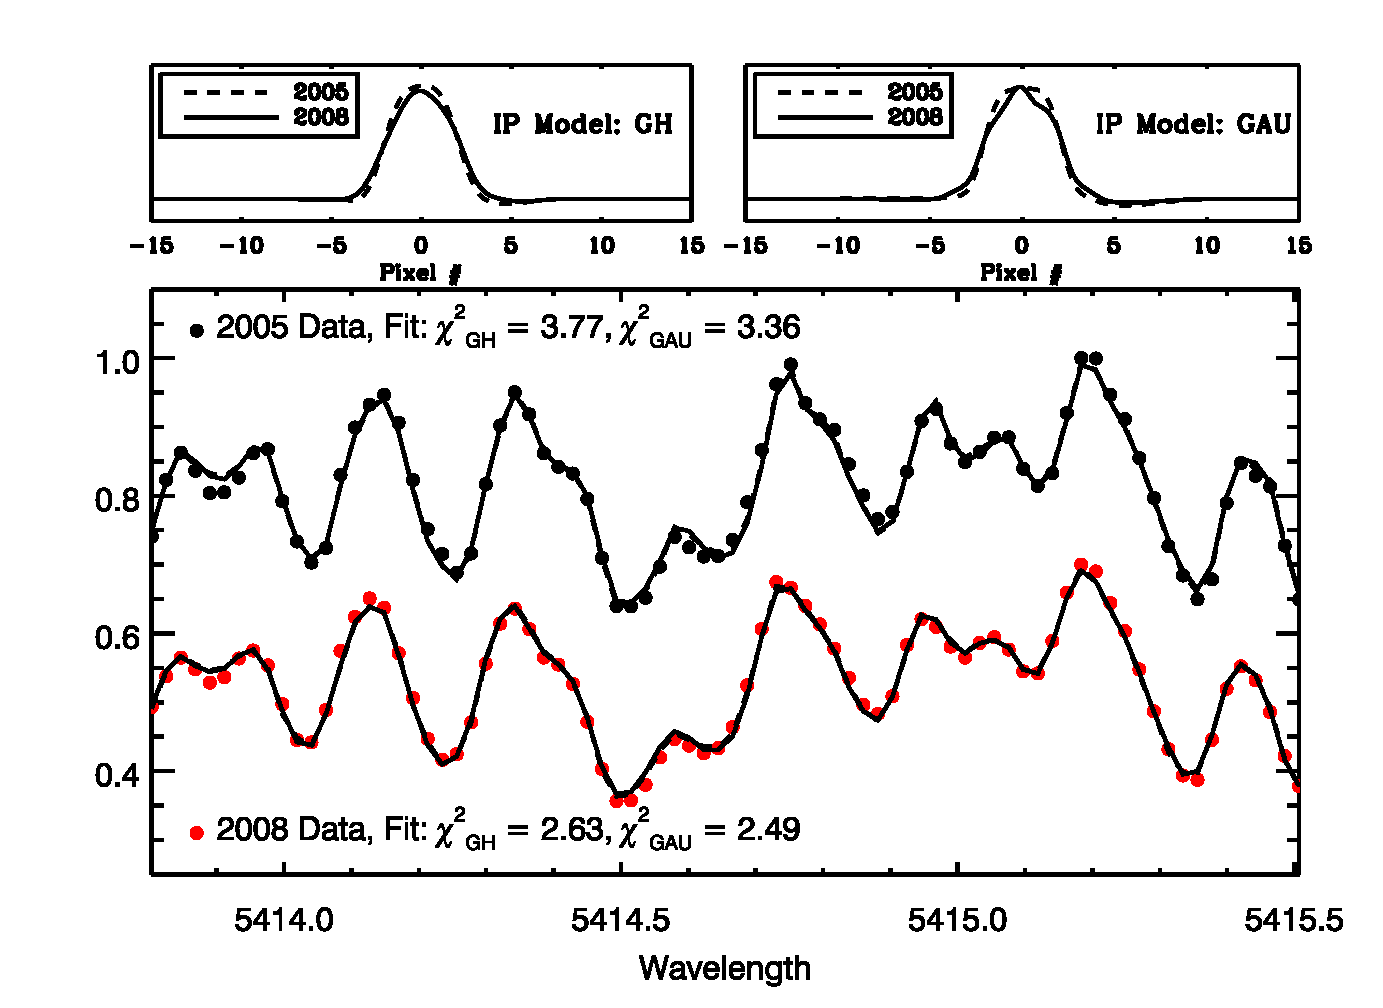
\includegraphics[scale=0.45]{het/iodfit.eps}
\caption{Illustration of fitting the iodine-only data (bottom panel)
  using different IPs (top panels), in this case, using GH and sum of
  Gaussians (GAU). These two IPs are practically ``equally bad",
  having similarly large reduced $\chi^2$ but neither produces a
  satisfactory fit. It is also interesting to see how ``stable" the
  best-fit IP can be across the years (i.e., in 2005 vs.~2008) and its
  smoothness, hinting that the best IP may take a simple, slowly-varying form. 
\label{het:fig:ghgau}}
\end{figure}
%----------------------------------------------------------------


We then looked for clues in the Fourier space:
Figure~\ref{het:fig:fftip} plots the Fourier transform power spectrum
of the \het\ data (using the {\it fft} procedure in IDL) for the
entire $\sim$1000\AA\ 1-D extracted spectrum used for precise-RV
purposes; with \keck\ data also plotted for comparison). At high
frequency in Fourier space, or shorter periods in pixel space, i.e.\
on small scales, the power spectrum is dominated by the signature of
the IP. A ``null'' in the power spectrum at 4.3 pixel is clearly
visible, which suggests some sort of sharp feature, and indeed, it
exactly corresponds to the slit width of \het\ projected onto the
detector at a resolution of R $=$ 60,000. This feature is a direct
result of the fact that HRS has the slit in front of a round fiber,
creating somewhat of a sharp feature in its IP, unlike the slit-fed
\keck.


%----------------------------------------------------------------
% Comparing Keck and HET IPs in Fourier space
% plot from screen shot of a slide in
% ~/ExoPlanet-2010-2011/Professional_Development/20150727-ThesisCommMeet/
% original plot is from ~/Exo../HET.../06-line.../powspec.pro and stored in ./plots/
\begin{figure}
\centering
\includegraphics[scale=0.35]{het/fftip.eps}
\caption{Fourier transform or power spectrum of a \het\ iodine-only
  spectrum (black dots) and its smoothed version (blue line). There is
  a clear signature of the \het\ slit at 4.3 pixel (corresponding to
  slit width for resolution R $=$ 60k). For comparison, the red curve
  is for \keck\ data, which shows no clear signature of a slit,
  because \keck\ is not fiber-fed and the PSF of the star falls mostly
  within its slit.
\label{het:fig:fftip}}
\end{figure}
%----------------------------------------------------------------


Upon seeing the Fourier transform of the \het\ data, we tried out
another IP using GH multiplying a triangle (with a half width of 2.4
pixel and a height of 1), whose Fourier transform has a null at 4.3
pixel, and it produced the best fit among all IP models we have
ventured. Figure~\ref{het:fig:iodipcomp} illustrates this new fit in
comparison with the GH IP fit, although it was perhaps
still equally bad. At this point, we have already suspected that
the ``ground truth'' for the iodine lines, the iodine atlas, which was
created from an FTS scan, may be problematic. It would not be possible
to derive a correct form for the IP using a wrong iodine atlas, and
thus we shift our priority towards validating the iodine cell FTS and
investigating possible changes in the cell, which is described in the
next section.


%----------------------------------------------------------------
% Comparing fits with two IPs: GH, and GH+triangle
% plot made by ~/Exo.../HET.../plots_general/fit_demo/compfit.pro
\begin{figure}
\centering
\subfloat{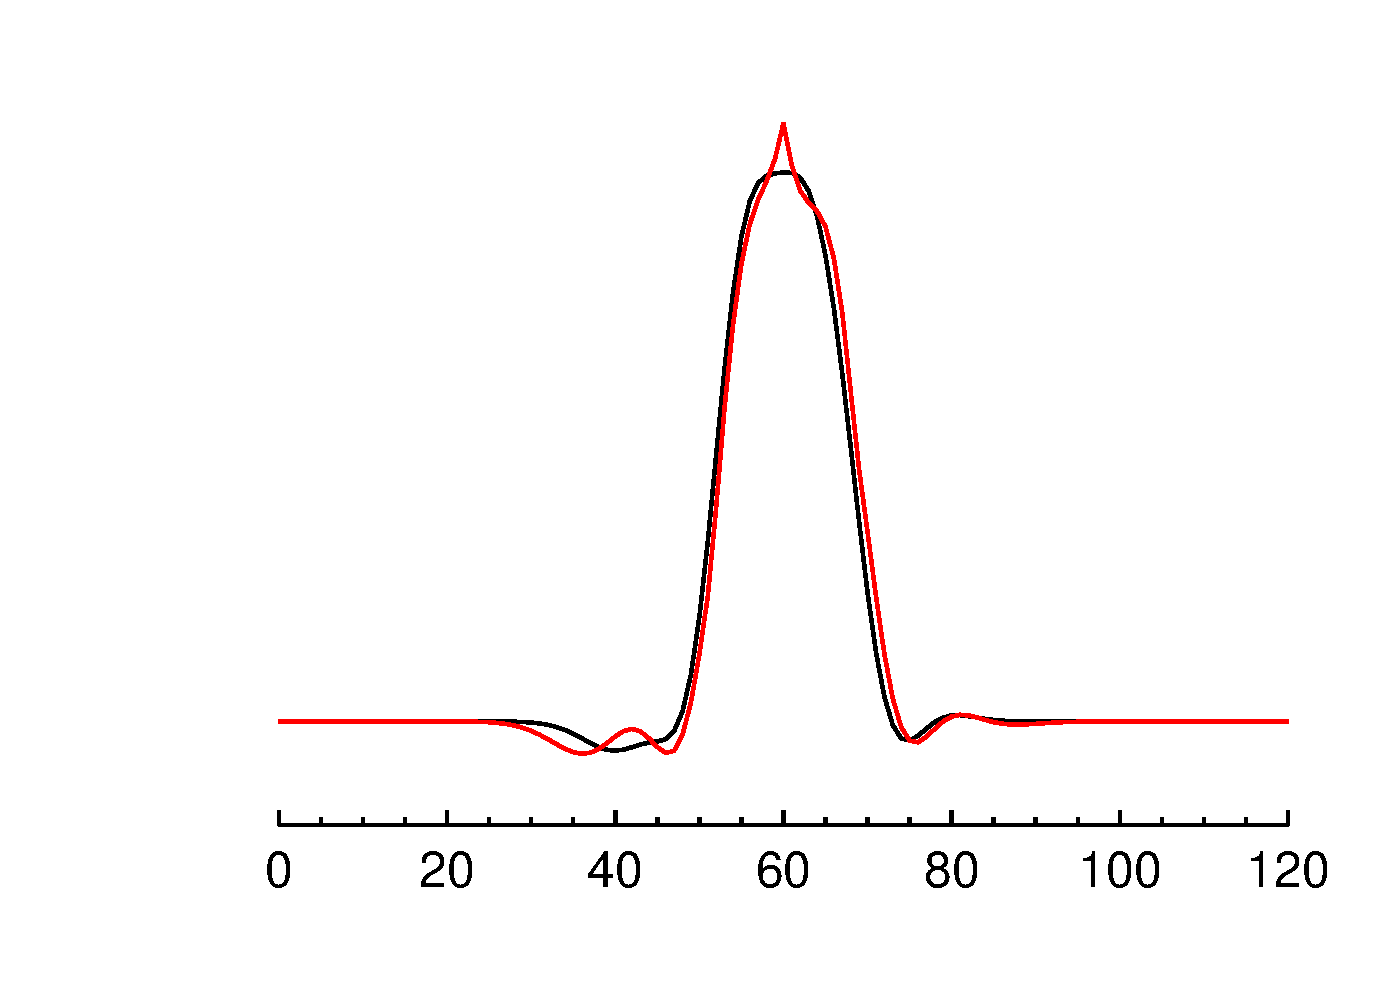
\includegraphics[scale=0.3]{het/20120124.176005.chunk191.compip.eps}}
\subfloat{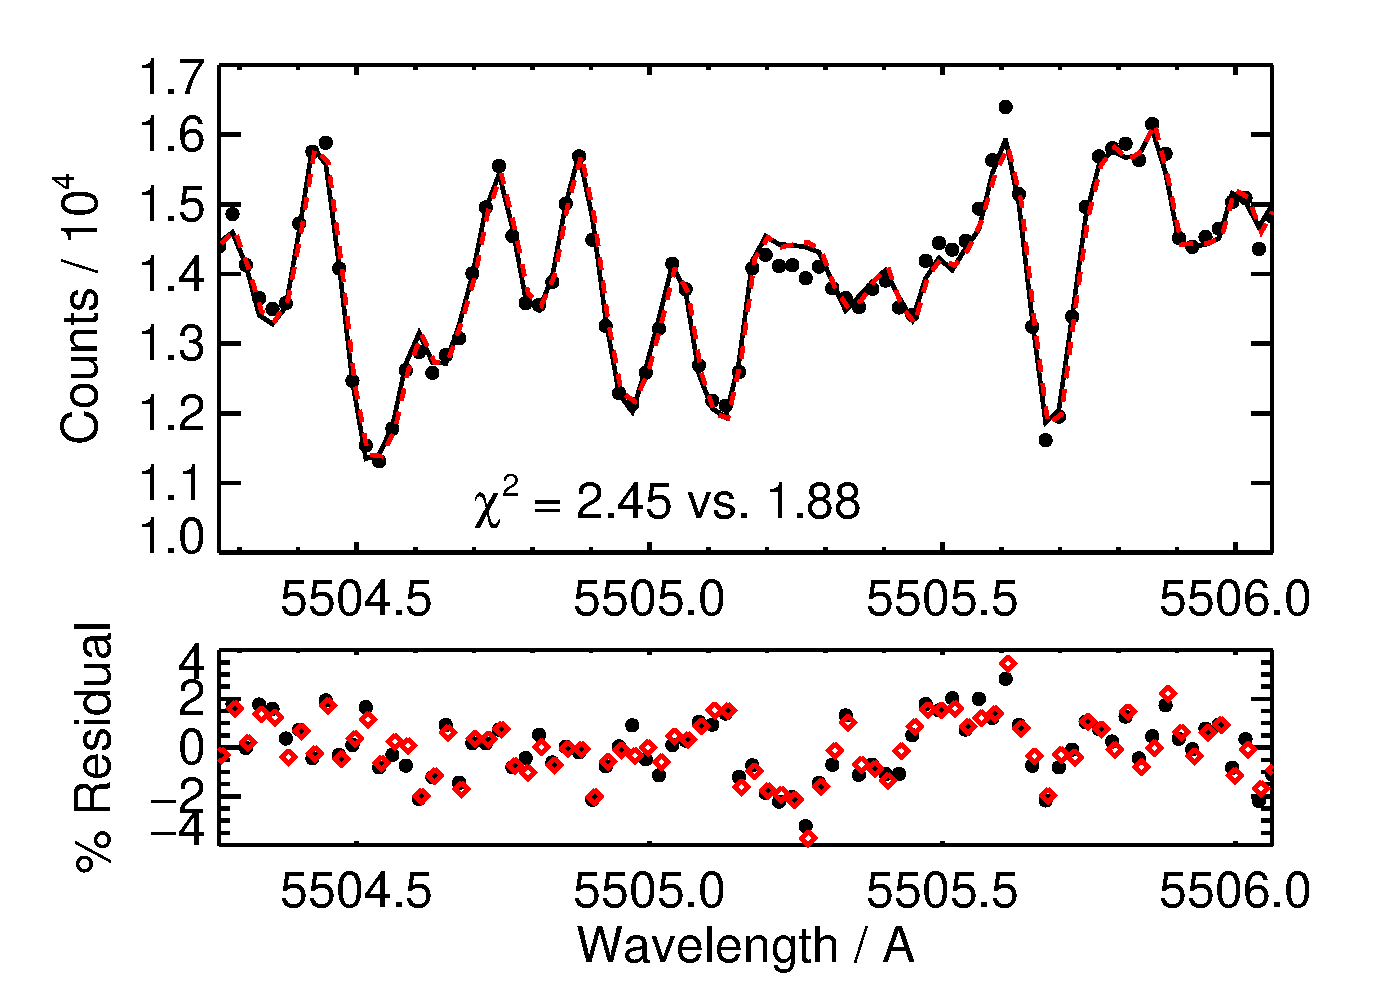
\includegraphics[scale=0.35]{het/20120124.176005.chunk191.compfit.eps}}
\caption{Introducing a sharp feature into the \het\ IP model, a
  triangle on top of the GH IP (red curve in the left panel), produces
  a better fit, somewhat to our surprise. The black in the left panel
  is the best-fit GH IP. GH$+$triangle is the IP model that produces
  the least $\chi^2_\nu$ among all of our IP models. However, as shown
  by the right panel, the two fits barely have any visible difference
  (red curve for GH$+$triangle IP and black for GH; bottom panel plots
  the residuals). Such a sharp feature in the IP is nonphysical, and we
  interpret this results as a hint for an unreliable iodine atlas
  (the sharp peak at the center is perhaps the IP model trying to
  ``stretch" the iodine lines deeper; see Section~\ref{het:sec:fts}
  for more details).
\label{het:fig:iodipcomp}}
\end{figure}
%----------------------------------------------------------------


Besides the problem with the iodine atlas, which fundamentally
prevents us from finding a precise IP, we know for sure that the GH
function does not work very well. We have two lines of evidence
supporting this statement. The first one is that the GH IP performs
terribly on \keck\ data because the L-M least-\chisq\ fitter has
trouble converging (unless fine-tuned and informed from previous fits
using sum of Gaussians; \citealt{2013AAS...22114908V}). The second
piece of evidence is that we tried to fit GH to unsaturated ThAr lines
in \het\ calibration frames, and it often fails to converge onto a
good fit to the ThAr line. 

To end this section with a somewhat positive note, we present a
promising lead for a better IP function for \hrs, the modified Moffat
function:
\begin{equation}
[1+(x/\theta)^2]^{-\beta\cdot(x/\delta)^2}
\end{equation} 
It is called the ``modified" Moffat function because the original
Moffat function does not have the $(x/\delta)^2$ term. We added this
term to add flexibility at the wings to enable change of
characteristic IP width while preserving wing
profile. Figure~\ref{het:fig:moffat} illustrates the results using the
modified Moffat fitting a ThAr line (insert), and also the
$\chi^2_\nu$ distribution of all spectral chunks for this new IP
compared with the GH IP. Unfortunately, the modified Moffat function
does not always fit a ThAr line (starting with uninformed initial
guesses), so it faces the same problem as GH. However, it only has
four parameters and they are mostly physically meaningful. For
example, one can imagine that the $\theta$ parameter describes some
characteristic width. This makes this function easier to work with than
GH.

One can image getting a better fit by adding small perturbation terms
to the modified Moffat IP to account for asymmetries and subtle wings
due to scattered light. Moreover, the modified Moffat function is
potentially applicable to other fiber-fed instruments, since such
instruments are likely to have IPs with the same characteristic flat
top and sharp wings. We hope to continue this effort after the iodine
atlas problem is resolved (see next section) and carry on this
knowledge to other projects such as the new HRS and MINERVA
(Chapter~\ref{chap:conclusion}).


%----------------------------------------------------------------
% Fitting with a Moffat function
% plot made by ~/ExoPlanet-2010-2011/HET-HRS-IP/06-line_through_dots/thar.pro
% and stored in ./plots/
\begin{figure}
\centering
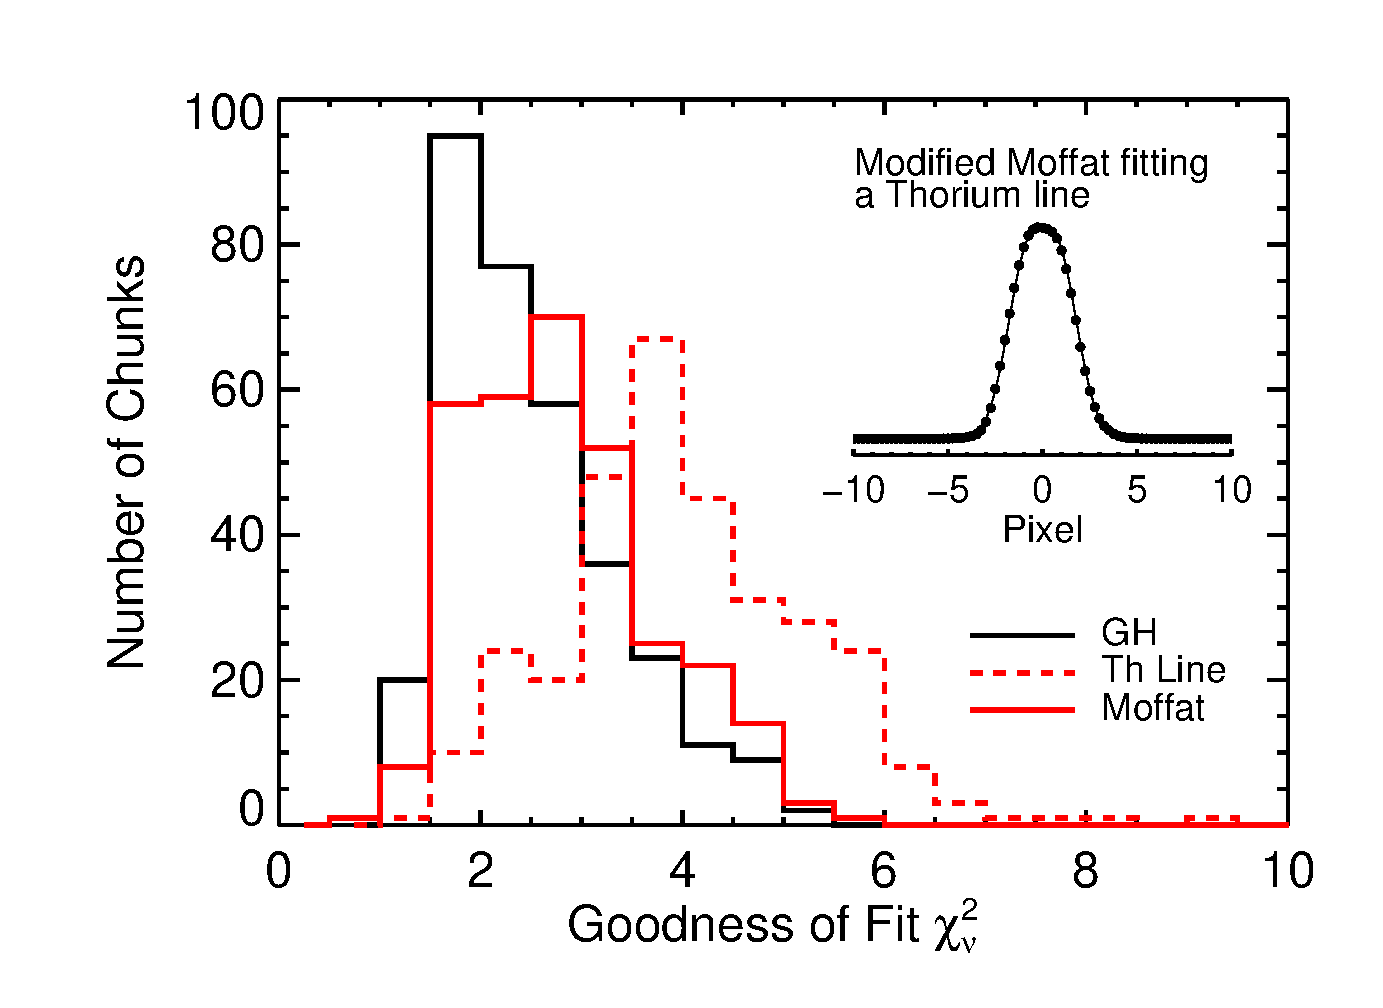
\includegraphics[scale=0.45]{het/thar_vs_moffat.eps}
\caption{Histogram of goodness of fit, $\chi^2_\nu$, values for
  spectral chunks of an iodine spectrum. The modified Moffat function
  (red) performs almost equally well while having only 3 parameters,
  com- pared with the complicated 11-parameter GH function (black
  solid). Red dashed histogram is for fits using a ThAr line profile
  as IP. The insert is showing the modified Moffat function can fit a
  ThAr line quite well.
\label{het:fig:moffat}}
\end{figure}
%----------------------------------------------------------------





%%%%%%%%%%%%%%%%%%%%%%%%%%%%%%%%%%%%%%%%%%%%%%%%%%%%%%%%%%%%%%%%%%%%%%%%%%%%%%
\section{Investigation on the Iodine Cell and the Iodine Atlases}\label{het:sec:fts}

% HET FTS

As discussed in the previous section, successful modeling of the
iodine observations (B star spectra taken through the Iodien cell) is
a good indication of a working radial velocity (RV) pipeline. At
Keck/HIRES, which has demosntrated 1 m/s RV precision over the years,
the modeling of the iodine observations yields a reduced chi-square
(\chisq) value of typically 1.05. However, for HET/HRS iodine
observations, with the same RV pipeline used at Keck, the typical
\chisq\ value is $>2$ or even $>5$ for some observations. 

We have explored one of the two model components for modeling iodine
observations, the choice of IP. In this section, we examine the other
model component, the iodine atlas, that is, the ``ground truth''
spectrum for the iodine absorption lines unique to the \het\ iodine
cell. A ``ground truth" iodine atlas is crucial for the precise iodine
radial velocimetry. It is used for modeling the observed iodine lines
in the stellar$+$iodine RV observation to anchor the absolute
wavelengths and the spectrograph response function. 


%%%%%%%%%%%%%%%%%%%%%%%%%%%%%%%%%%%%%%%%%%%%%%%%%%%%%%%%%%%%%%%%%%%%%%%%%%%%%%
\subsection{Why did we suspect the iodine atlas?}

As we were investigating the reasons behind the apparent `bad fit' of
\het\ iodine observations, we decided to check the quality of the
existing iodine atlas. An iodine atlas is normally obtained using a
Fourier Transform Spectrometer (FTS; whose mechanism is just like a
Michelson interferometer). The scan and its subsequent data reduction
provides very high resolution spectrum (translated from Fourier space
into real space) with typically $R > 200,000$-500,000.\footnote{It is worth
noting here that although FTS normally provides wavelength solutions
(from the registered arm lengths), but because of the inaccuracy of
the default reported wavelengths, the final wavelength solution for
the iodine atlas is usually derived from a theoretically computed iodine
line list (e.g., \citealt{iodinespec5}).}

The existing iodine atlas for the \het\ cell is from an FTS scan taken
at the National Solar Observatory at KPNO using the Babar FTS
(nicknamed for its large size; this machine has been decommissioned)
in 1993. The main reason is that the FTS scan was taken almost two
decades ago, and during this time the cell may have gone through
changes (such as temperature, leaking or condensation, etc., though
unlikely, since the cell was designed to be stable). This would mean
that the FTS scan is out of date and inaccurate, and it could explain
the `bad fits' to the iodine observation.

We therefore took the HET/HRS cell to the National Institute of
Standards and Technology (NIST) and obtained a new FTS scan in 2011
(an effort carried out by Jason Wright, Ming Zhao, Stephen Redman and
others at NIST; data reduction done by Stephen Redman). A close
comparison between this new scan from NIST and the old scan at KPNO
reveals that they have many differences:
\begin{itemize}
  \item The overall line depths are very different --- the NIST scan
    has deeper lines.
  \item The absolute wavelength solutions are different, and the
    drifting of wavelength solution or the dispersion scales at
    different wavelength are also different.
  \item Even after we adjust the `normalization' level of the NIST
    scan (assuming the FTS data has normalization issues or low
    frequency noise/offset), the line ratios of the two scans still
    exhibits differences.
\end{itemize}

Figure~\ref{fig:fts_old_new} shows the comparison between the two
scans in a selected 2\AA\ region. As the two scans also differ in
resolution (the NIST scan has a higher resolution), the middle panel
is a more direct comparison: the NIST scan has been convolved down to
the same resolution with the KPNO scan; it is also shifted in
wavelength space so that the two scans match in absolute wavelength
solution; and it is adjusted to a different ``normalization'' level to
match with the KPNO scan as much as possible in order to compare their
relative line ratios.

    
%----------------------------------------------------------------
% Figure: HET FTS, KPNO old scan vs. NIST new scan
\begin{figure}[!th]
\centering
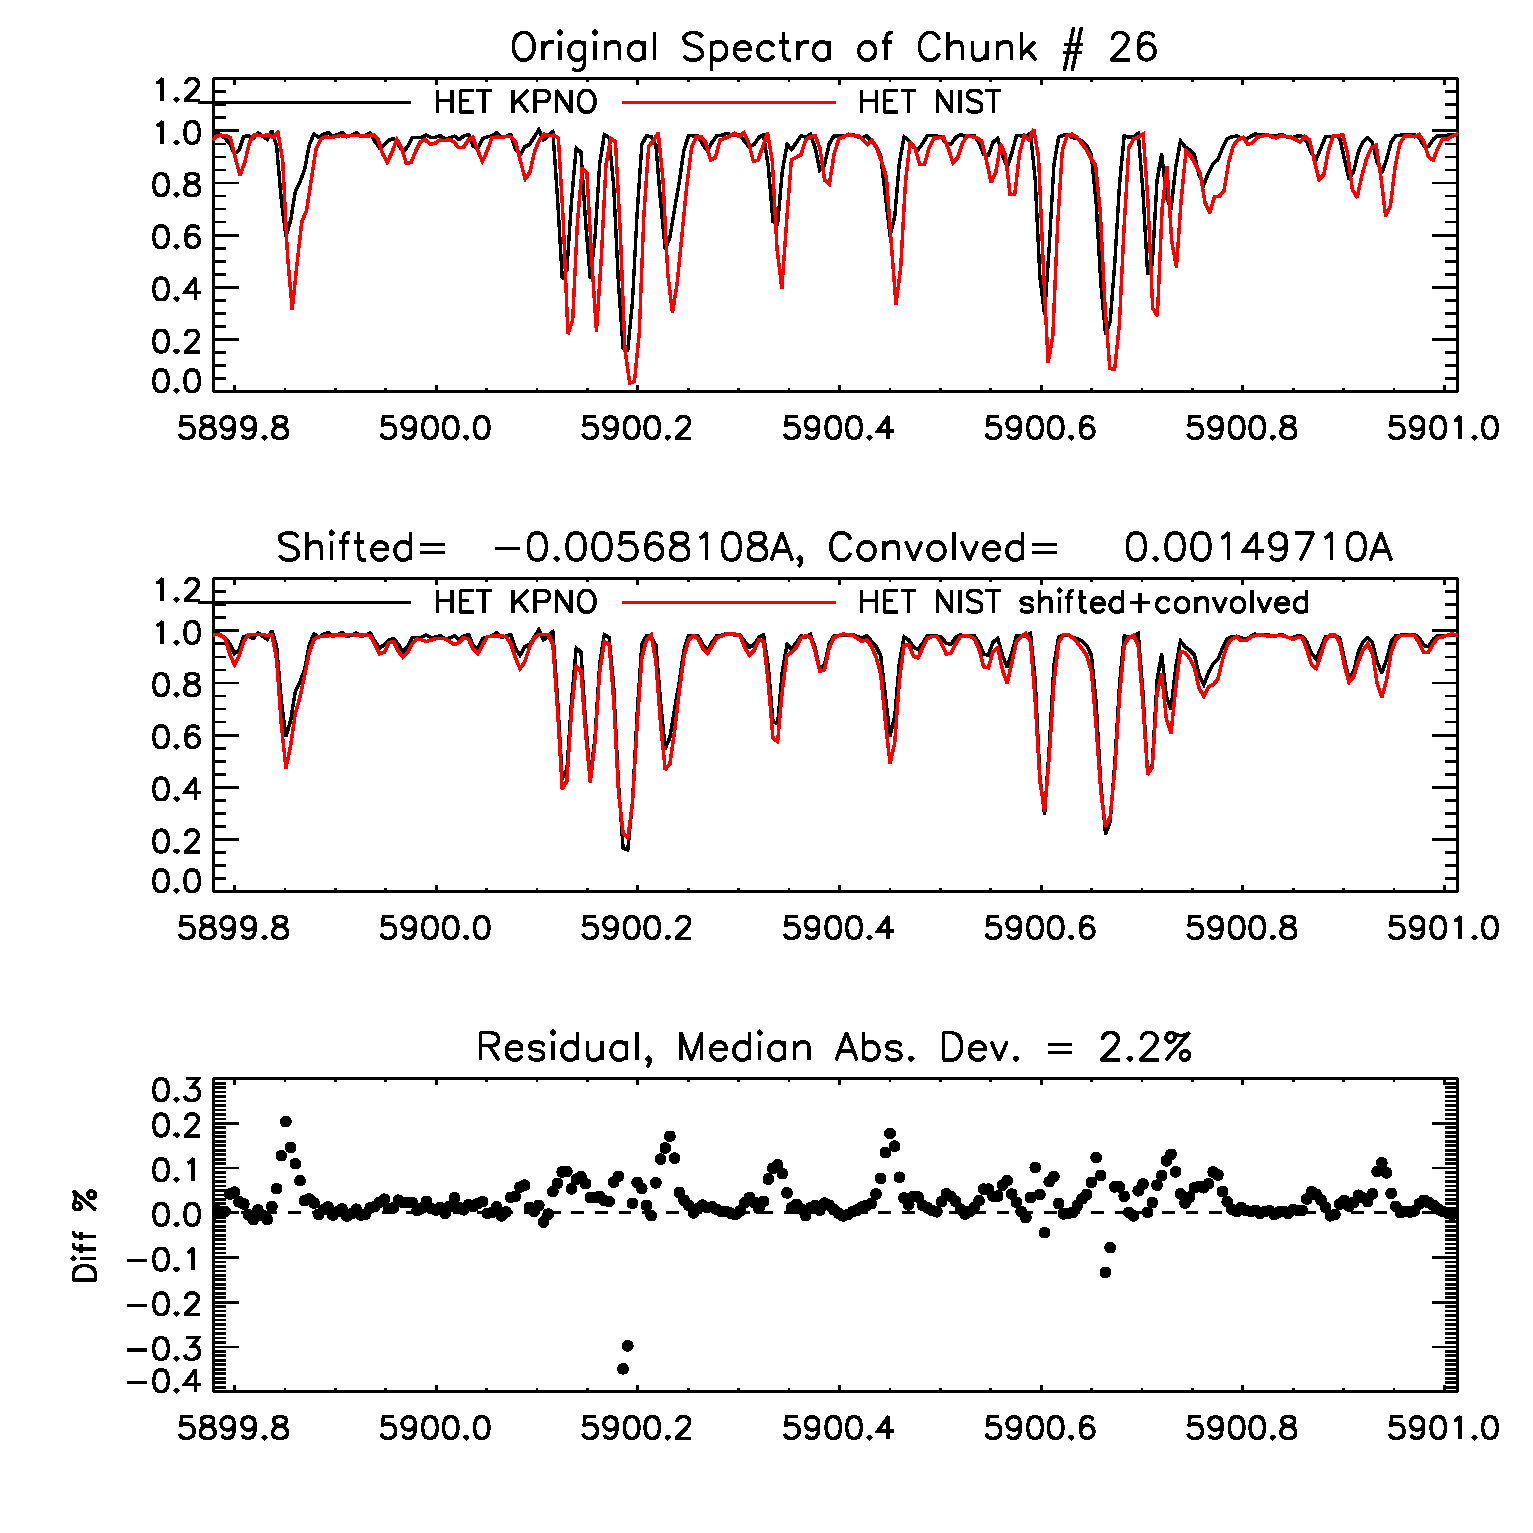
\includegraphics[angle=0.,scale=0.45]{het/compare_het_fts_26.eps}
\caption{Comparison of the KPNO FTS scan (black) and the NIST FTS scan
  (red) for the HET/HRS iodine cell for a selected
  1.5\AA\ chunk. \textbf{Top:} Two scans at their native resolution
  and original wavelength solution. \textbf{Middle:} Comparison of the
  two scans after adjusting the normalization, shifting, and
  convolution for the NIST scan to match the KPNO scan for a more
  direct comparison of line depths/ratios. \textbf{Bottom:} Residuals
  of the middle panel, NIST spectrum minus the KPNO spectrum. The
  median absolute deviation between the two spectra is 0.02
  (2\%), though at many places, especially at line centers, the two
  can differ by up to 5--10\%.
  \label{fig:fts_old_new}}
\end{figure}
%----------------------------------------------------------------

We initially suspected that the NIST scan was problematic. The reason is
illustrated in the left panel of Figure~\ref{fig:chisq_old_new}, where
it shows the histogram of \chisq\ values for fitting an selected iodine
observation using the two scans, respectively. Each \chisq\ value is
for a 2\AA\ chunk in this selected iodine observation. It is clear
that the NIST scan provides worse fits.

%----------------------------------------------------------------
% Figure: chisq of iodine observation fit, KPNO old scan vs. NIST new scan
\begin{figure*}[!th]
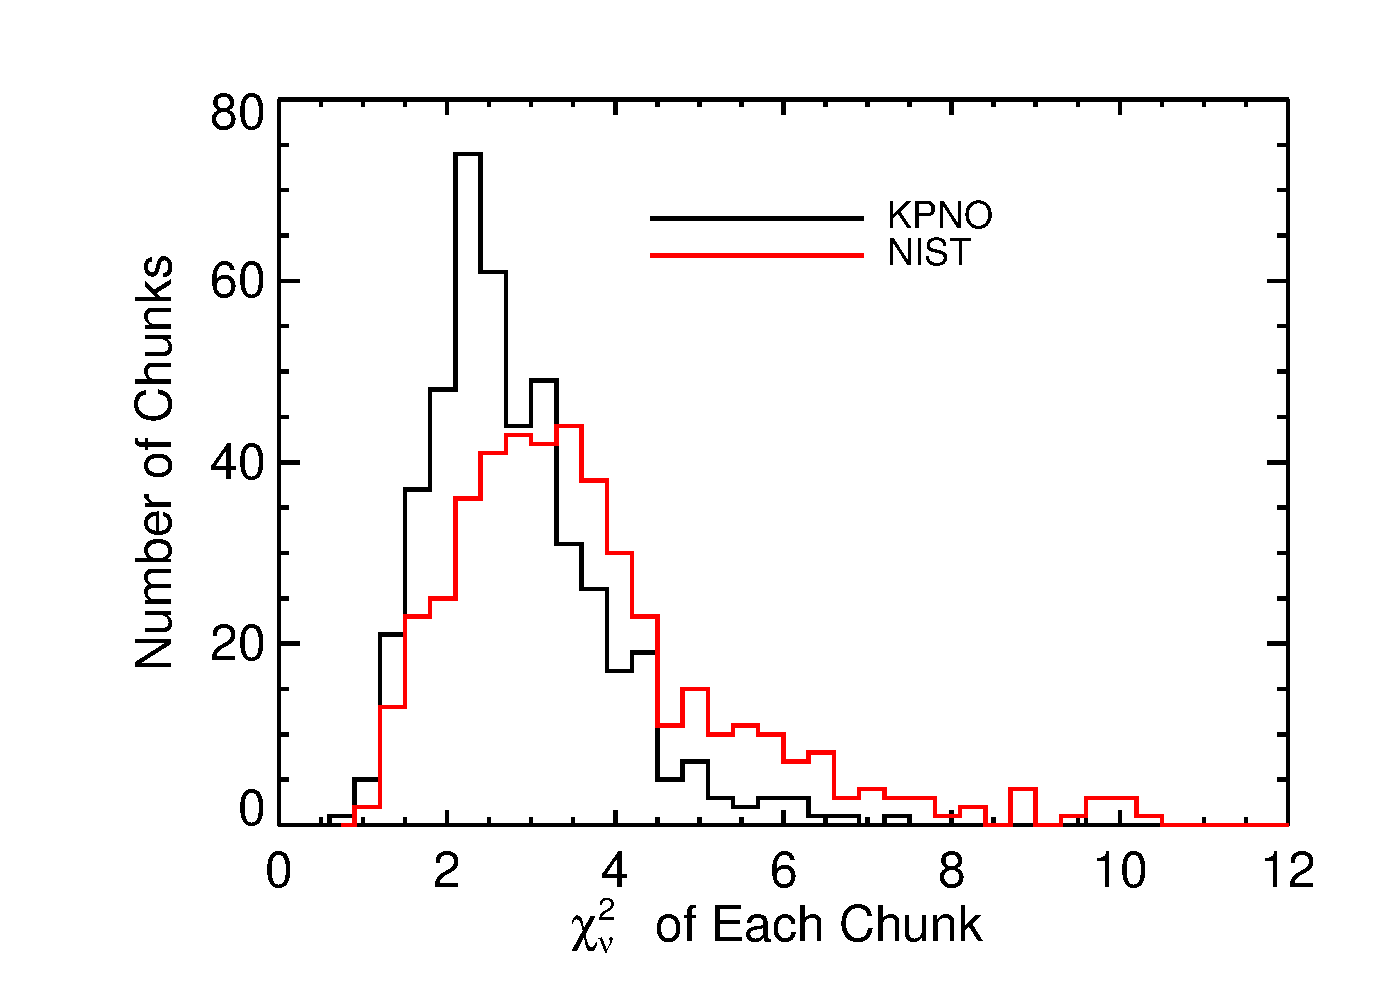
\includegraphics[angle=0.,scale=0.33]{het/hetfts_oldVSnew_chisq.eps}
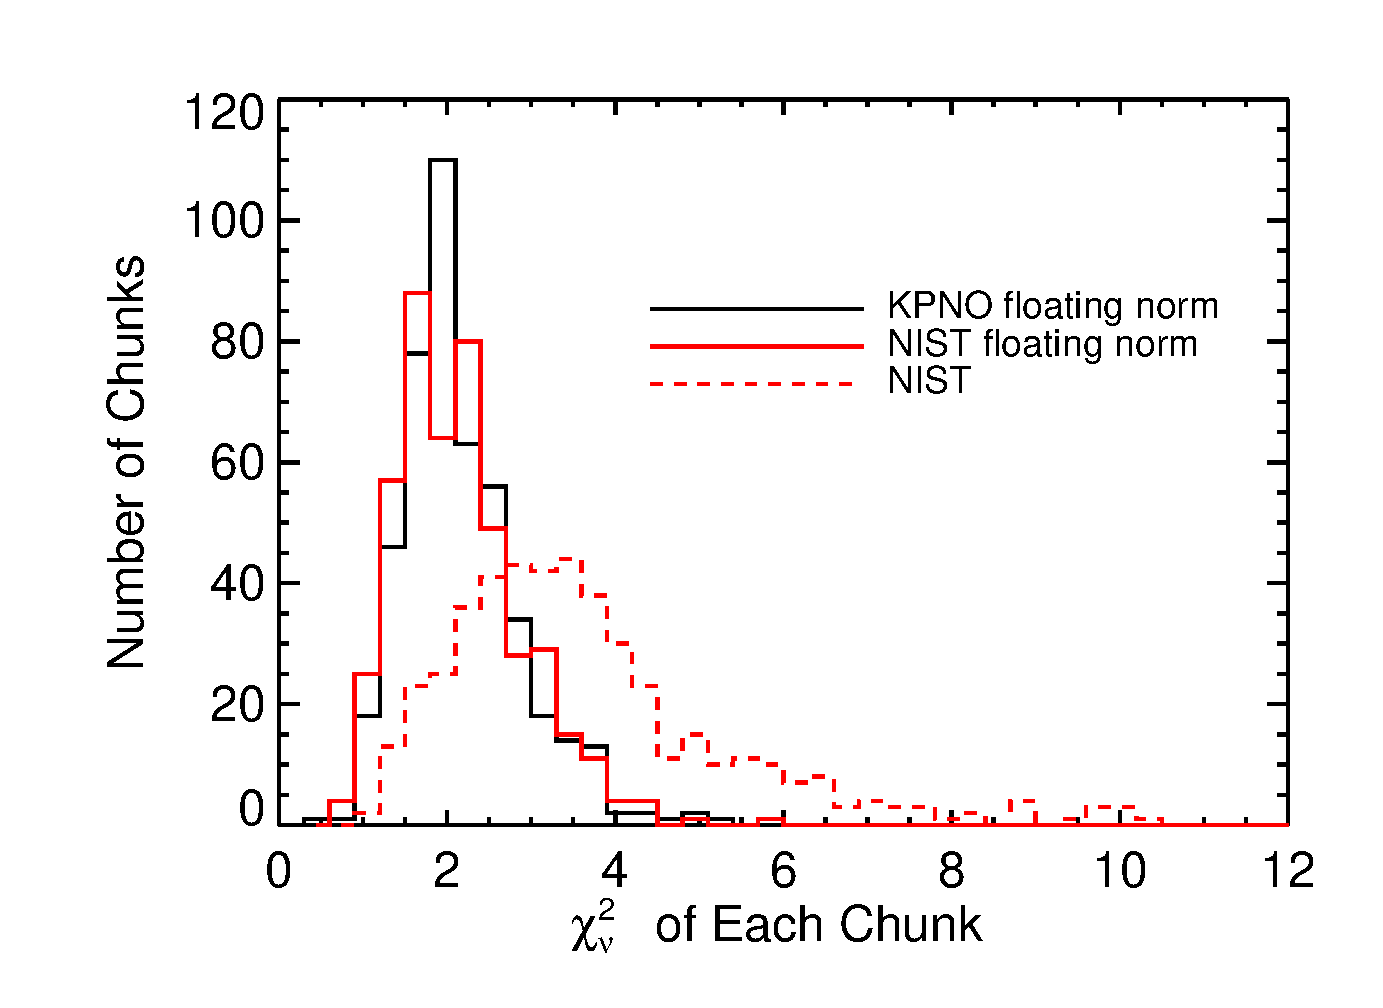
\includegraphics[angle=0.,scale=0.33]{het/hetfts_oldVSnew_chisq_dc.eps}
\caption{Both plots are histograms of \chisq\ values of a single
  iodine observation. Each \chisq\ value in the histogram represents
  the \chisq\ goodness of fit for a $\sim$2\AA\ spectral chunk in this
  iodine observation (each iodine observation is chopped into several
  hundred of chunks and is fitted independently).
%
  \textbf{Left:} \chisq\ histograms for the fit of the iodine
  observation using the KPNO (black) and NIST (red) scan as iodine
  templates, respectively. The KPNO scan obviously performs better.
%
  \textbf{Right:} \chisq\ histograms for the two scans, but both with
  the normalization as a free parameter for each chunk (as we suspect
  the NIST scan has problems in normalization). The two scans now
  perform at essentially the same level. Dashed red line is the same
  red histogram as plotted in the left panel. Notably, the KPNO scan
  also performs better when we float the normalization parameter.
  \label{fig:chisq_old_new}}
\end{figure*}
%----------------------------------------------------------------


Since the direct comparision between the KPNO scan and the NIST scan
has hinted that the `normalization' of the NIST scan might be
problematic, we decide to add a free parameter to account for this
`normalization error' when fitting the iodine observation. The right
panel of Figure~\ref{fig:chisq_old_new} shows the \chisq\ histograms
for the same iodine observation using the two scans, but adding a free
parameter as the `normalization' when fitting each chunk (note: the
normalization parameter is a free parameter for each chunk, not a
global single parameter). The two scans now perform at essentially the
same level.

This is both encouraging and worrisome at the same time. It is
encouraging because it seems that we have found the problem with the
NIST scan, and also have a solution for it. It is very worrisome
because this reveals that:
\begin{itemize}
  \item Even the KPNO cell performs visibly better when we float the
    normalization paramter. This may suggest that there are
    ``normalization'' issues or low frequency errors/noise in the KPNO
    scan as well.
  \item Obtaining high-quality, reliable FTS scans of iodine cell is
    very difficult, and the FTS scans cannot be naively trusted as the
    ``ground truth'' super accurate templates of the complicated iodine
    spectrum.
  \item The reason why adding a ``floating normalization'' fits the
    data better might be because it accounts for optical depths difference
    between the atlas and the actual observations, which may be a result
    of changes in cell temperature or iodine column density in the cell.
  \item The pipeline (when floating normalization as a free parameter)
    cannot distinguish which scan is the ``correct'' one (by \chisq)
    even when two scans differ as much as $\sim$5--10\% at places and
    also have obvious line ratio differneces (see comparison in bottom
    panel of Figure~\ref{fig:fts_old_new}). However, this level of
    difference in FTS may affect the RV precision, and not knowing
    which atlas is the correct one definitely affects our ability to
    search for a better IP and improve the RV precision of \het.
\end{itemize}  

Perhaps even more alarmingly and more puzzling, when we use the KPNO
scan for the iodine cell used at Keck/HIRES to fit an HET/HRS iodine
observation, it yields smaller \chisq\ values than using any of the
other two scans (Figure~\ref{fig:lampi2fit}). The \het\ cell KPNO scan
was taken at the same time using the same FTS machine as the \keck\
cell scan. However, the set-temperatures of these two cells are very
different: the \keck\ cell is designed to work at 50$\degree$C, while
the \het\ cell is designed to work at $70\degree$C. A closer look
reveals that the HET KPNO scan and the Keck KPNO scan have very
similar line depth, with Keck having slightly deeper lines (thus
higher iodine molecule column density).


%----------------------------------------------------------------
% Figure: chisq of iodine observations, NIST vs. KPNO vs. Keck cell 
% plots made by
% ~/ExoPlanet-2010-2011/HET-HRS-IP/05-Iodine_FTS_investigation/compare_fts/compare_fts_fits.pro
% stored in ../plots/
\begin{figure}[!th]
\centering
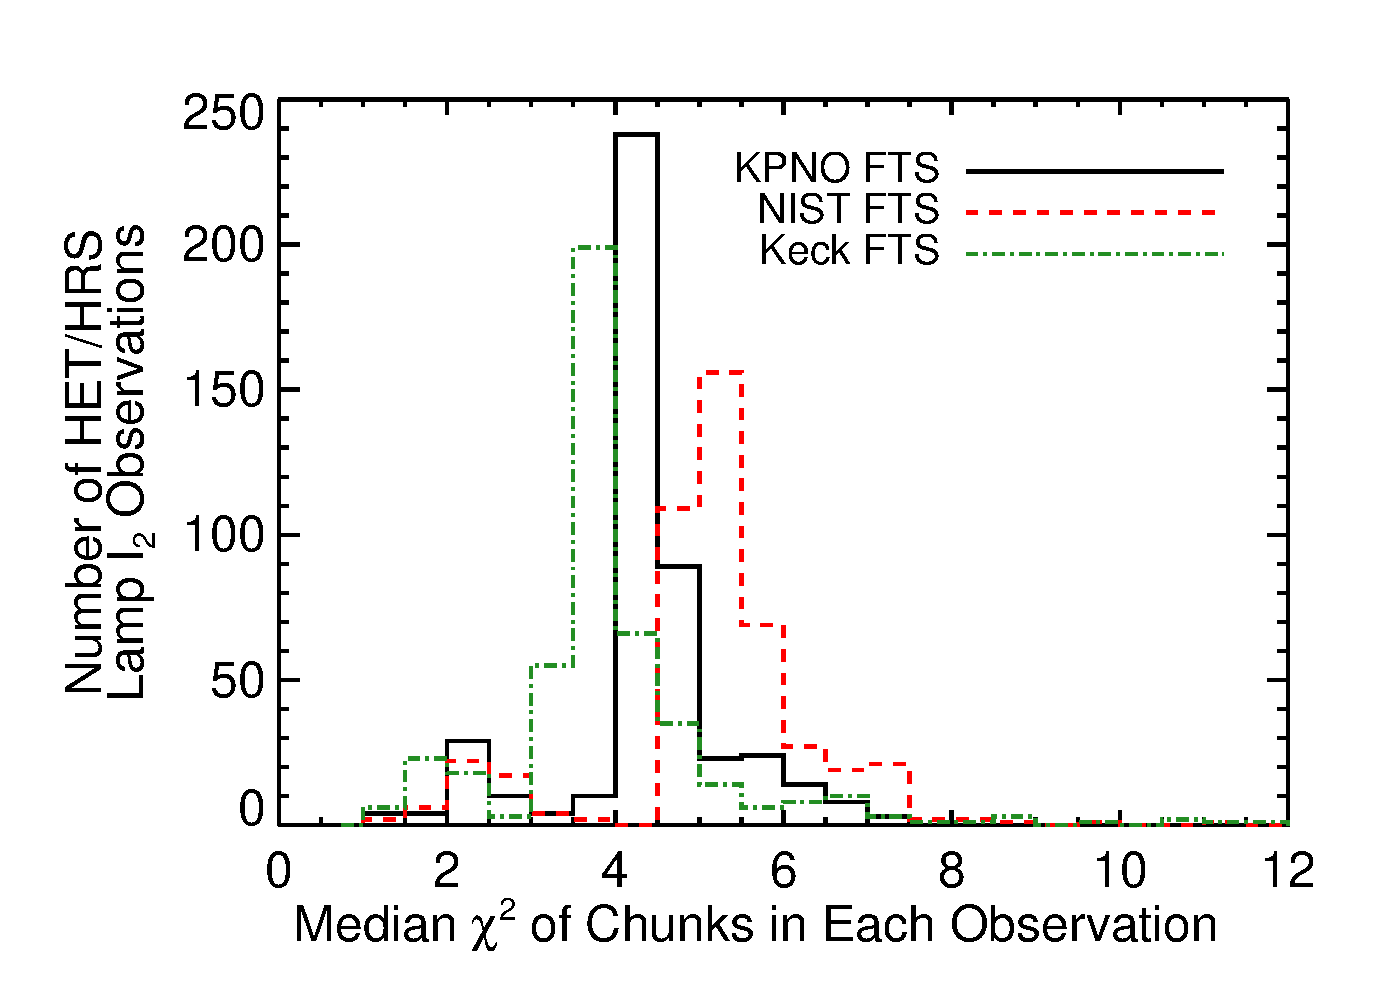
\includegraphics[angle=0.,scale=0.38]{het/het_lamp_i2_fits_kpno_nist_keck.eps}
\caption{Comparison of the median \chisq\ values for fits of iodine
  observations using the \het\ cell KPNO scan (black solid line), the
  NIST scan (red dashed), and the {\em \keck\ cell} KPNO scan (green
  dotted-dashed). Each data point represents the median \chisq\ value
  for all the chunks in a single iodine observation (these are all
  lamp-illuminated -- no B star observation). Results of 550
  \het\ observations are plotted here to illustrate the statistically
  significance. The \keck\ cell KPNO scan provides a better fit than the
  both \het\ scans when fitting \het\ iodine observations.
  \label{fig:lampi2fit}}
\end{figure}
%----------------------------------------------------------------

All of the facts above prompted us to seek a relatively
independent way to perform quality checks for any FTS scan --- not
just comparing their relative qualities or performances. One
natural choice is to obtain spectra taken with high-resolution echelle
spectrographs, which are measurements of the iodine spectrum directly
in the ``real wavelength space'' instead of in the ``Fourier space'', and
thus they serve as good reference spectra as they suffer from
different types of error compared to FTS. Since FTS scans are usually
at a very high spectral resolution ($200,000$--$500,000$), this limits
our choice to essentially only one spectrograph --- the TS12 setting
of the Tull Spectrograph at the 2.7m Telescope at McDonald.

Our goal is to answer the question of {\bf which FTS scan better describes
the \het\ iodine cell: the KPNO one, or the NIST one? Why?} While adding an
additional normalization parameter can provide better fits for the
iodine frames, we cannot afford to add such an additional parameter
when extracting RVs from star$+$iodine data -- this normalization
parameter is highly degenerate with Doppler shift and wavelength
solution parameters, and it will undoubtedly decrease the RV
precision. Another key question is {\bf why the FTS scan for the \keck\
cell works the best.}


%%%%%%%%%%%%%%%%%%%%%%%%%%%%%%%%%%%%%%%%%%%%%%%%%%%%%%%%%%%%%%%%%%%%%%%%%%%%%%%%%%%%%%%%%%%%%%%%%%%%
\subsection{Ultra-High Resolution Echelle Spectra of Iodine Cells}

To break the tie between various FTS scans, we used the TS12 setting
of the Tull Spectrograph at the 2.7m Telescope at McDonald
Observatory, which provided a resolution of 500,000 (based on ThAr
line measurements done by David Doss at McDonald). 

We had two rounds of TS12 runs, both during day time and when the
telescope was scheduled to on Cassegrain instrument and the Tull
Spectrograph room was free for use. For the first run (from September
7 to September 9, 2013; done by Ming Zhao and the author) we measured
the iodine absorption spectrum for the iodine cell at the Sandiford
(2.1m) Telescope, because the HET/HRS cell was still under active use
when we did this test. The main purpose of the first run was to
validate the quality of the TS12 spectrum and whether we can use it to
across-validate the FTS scans. The Sandiford cell also has an KPNO FTS
scan which was taken together with the KPNO scan of the HET cell in
1993, so it also serves the purpose of testing the overall quality of
the KPNO scans.

In the second TS12 run, we measured the spectrum for the \het\ iodine
cell in its new enclosure and temperature controller (along with the
MINERVA iodine cell and the iodine cell on McDonald Harlan J.\ Smith
2.7m telescope; from October 13 through October 16, 2014; carried out
by Ming Zhao, Kim Star, and Joey Schmitt). Our TS12 runs are enabled
by Anita Cochran, Bill Cochran, Phillip MacQueen, and the astronomers
who used the Cassegrain instruments at night (VIRUS-W for the first
run and IGRINS for the second), with great help and excellent
engineering support from David Doss and Coyne Gibson at McDonald
Observatory.

The hardware settings and data reduction methods are the same for both
runs, which are described below.

\textbf{\textit{Hardware Settings:}} We used the TS12 arm of the Tull
Spectrograph, and the specific instrument choices are listed in
Table~\ref{tab:hardware}. Slit \#23 is chosen to maximize SNR while
maintaining sufficient resolution --- it is among the longest slit and
is also the second narrowest slit. The Sandiford cell was kept at a
temperature of 49.9--50.1$^\circ$C, the same as its working
temperature for RV work and its temperature when the KPNO was taken
(50$\degree$C). The \het\ cell was measured at four different
temperatures: room temperature, 50$\degree$C, 60$\degree$C, and
70$\degree$C (its working temperature). 

%----------------------------------------------------------------
% Table: variability analysis results
\renewcommand{\arraystretch}{1.3} % more row spacing for the table
\begin{deluxetable}{rl}
%\rotate
\tabletypesize{\scriptsize}
\tablewidth{180pt}
\tablecaption{Hardware Settings for TS12 Iodine Spectrum Test\label{tab:hardware}}
\startdata
  \hline
  \multicolumn{2}{c}{Tull Spectrograph, TS12, Coude107} \\
  \hline
  Echelle & E1 \\
  Cross Disperser & c \\
  CCD & TK4, 1024$\times$1056 \\
  On-chip Binning & 1$\times$1 \\
  Slit & \#23 (L$\times$W $=30\arcsec \times 0\arcsec .32$)
\enddata
\end{deluxetable}
%----------------------------------------------------------------


\textbf{\textit{Observation:}} A single exposure frame for the iodine
spectrum covers about 1.9\AA\ (Figure~\ref{het:fig:ts12image}). The
dispersion direction runs vertically along the chip with increasing
wavelength when increasing the $y$-axis pixel. The dispersion scale is
about 0.002\AA\ per pixel ($\sim$7 pixels per resolution element). We
immediately preceded or followed each exposure with a flat fielding
frame. The exposure times for the iodine and flat frames are both 45
seconds (90 seconds for \het\ cell) to achieve a signal-to-noise ratio
(SNR) of 160 per pixel (higher for \het\ cell). Neighboring frames
differ by about 1\AA\ in absolute wavelength. If prominent Solar or
ThAr line was predicted within the wavelength coverage of a frame,
then we also took a Solar or ThAr frame to verify the rough wavelength
solution (the exposure time varied --- typically a couple minutes to
up to 10 minutes). We took dark frames (45s each, about 10 frames) in
the morning at the beginning of each day.

%----------------------------------------------------------------
% TS12 raw image
% plot made by ds9 view on spec0248.fits in
% /Volumes/galileo/rv/TS12/raw/, i.e. 2013 data, save as jpg then
% converted online into eps
\begin{figure}
\centering
\includegraphics[scale=0.35]{het/ts12_image.eps}
\caption{One raw image frame taken using the TS12 setting of Tull
  Spectrograph. It contains about 1.9\AA\ of iodine absorption spectrum. 
\label{het:fig:ts12image}}
\end{figure}
%----------------------------------------------------------------


\textbf{\textit{Reduction:}} We combined and averaged all available
dark frames and created a master dark frame. Then we subtracted the
master dark from all flat and iodine frames. After outlier rejection
(cosmic rays, chip defects, etc.), we modeled the scattered light for
each row of pixels by using the region outside the slit image.  We
stacked 160 neighboring rows and fitted a third order polynomial along
the column, and then interpolated for the amount of scattered light
within the slit image region and subtracted it. Both the flat and
iodine frames have scattered light removed. We then normalized the
flat frames and divided each iodine frame by its associated normalized
flat (for the slit image regions only).

\textbf{\textit{Extraction:}} As the slit does not lie perfectly along
the $x$-axis direction on the chip, we corrected for this by cutting
columns along the dispersion direction and cross-correlating the
columns. Then we interpolated and shifted the columns to create an
aligned image, which we stacked along the $x$-axis direction and
obtained the reduced, extracted spectrum. Each spectrum is then
normalized by dividing the estimated continuum (top 5\% counts). Due
to lower quality of scattered light removal near the edge of the chip,
we discarded the top 80 and bottom 80 rows of pixels. Thus the
extracted spectrum from each frame is about 1.6\AA\ across (instead of
1.9\AA). The reduced frames are then `stitched' together by finding
the overlapping region through cross correlation for each pair of
neighboring frames and taking into account the changes and differences
of dispersion scales across frames.
\begin{comment}
For the overlapping region, the spectrum in the bluer frame is
`projected' onto the redder frame by taking into account the changes
and differences in pixel dispersion scales in the two frames. The
overlapping spectral region in the stitched spectrum thus has the
dispersion scale of the redder frame, but it preserves the
normalization of the bluer frame. This way the two frames are stitched
together.
\end{comment}

\textbf{\textit{Mapping onto FTS:}} To compare with the FTS
scans, we chopped the TS12 spectrum into 2\AA\ chunks and project
each chunk onto the FTS spectrum by cross correlation. In this way we
obtained the absolute wavelength solution and dispersion scale (as set
by the wavelength solution of the FTS scan) for the TS12
spectrum.

The results from our first TS12 run using the Sandiford cell
demonstrated that an iodine cell spectrum taken with TS12 has the same
quality as an FTS scan to serve as the `true solution' of the iodine
spectrum. The left panel of Figure~\ref{fig:ts12} shows a direct
comparison of the reduced TS12 spectrum (a random 2\AA\ chunk) with
the KPNO FTS scan, at their native resolutions.\footnote{Note that the
TS12 spectrum appears to have a higher resolution than the FTS
scan. According to the header of the FTS scan, its resolution is about
$491,000$. An FFT analysis on the TS12 spectrum (to see where the
high-frequency signal cuts off and becomes indistinguishable from the
noise) shows that its resolution is about $455,000$ and maybe even
higher.}

To make a more direct comparison and also to see the differences of
the two spectra (if any) would make a significant impact when fitting
a $60,000$ resolution iodine observation, we degraded the resolution
of both spectra to $60,000$ by convolving them with a Gaussian of a
proper width. The right panel of Figure~\ref{fig:ts12} illustrates the
comparison of the two spectra at $R\sim60,000$, with residuals of the
TS12 spectrum minus the KPNO FTS spectrum plotted in the bottom
panel. The two spectra differ by a median absolute deviation of 0.3\%
($0.4\%$ for the entire $\sim$30\AA\ spectrum available as shown in
Figure~\ref{fig:60k_all}).\footnote{ For comparison: when fitting the
HET/HRS Iodine observation used for creating
Figure~\ref{fig:chisq_old_new} (median SNR for a typical chunk is
$\sim$150, or 0.65\% shot noise), for a typical chunk, the median
absolute deviation between the observation and the best-fit model is
0.73\% (the RMS value is 1\%, thus \chisq\ is $\sim 2$--$3$).  } As
the TS12 spectrum has a SNR of about 160 and we have convolved the
comparison spectrum down to $R\sim60,000$, the expected shot noise
should be $\sim 1/160\times \sqrt{450,000/60,000}=0.23\%$. The
additional $\sim 0.1\%$--$0.2\%$ of noise may come from flat fielding,
scattered light removal, cosmic ray removal and interpolation between
pixels, stitching of spectra, projection onto the FTS spectrum and
interpolation for comparison purposes, and so on.


%----------------------------------------------------------------
% Figure: TS12 spectrum vs. KPNO FTS scan, native resolution, selected
% 2A chunk
\begin{figure*}[!th]
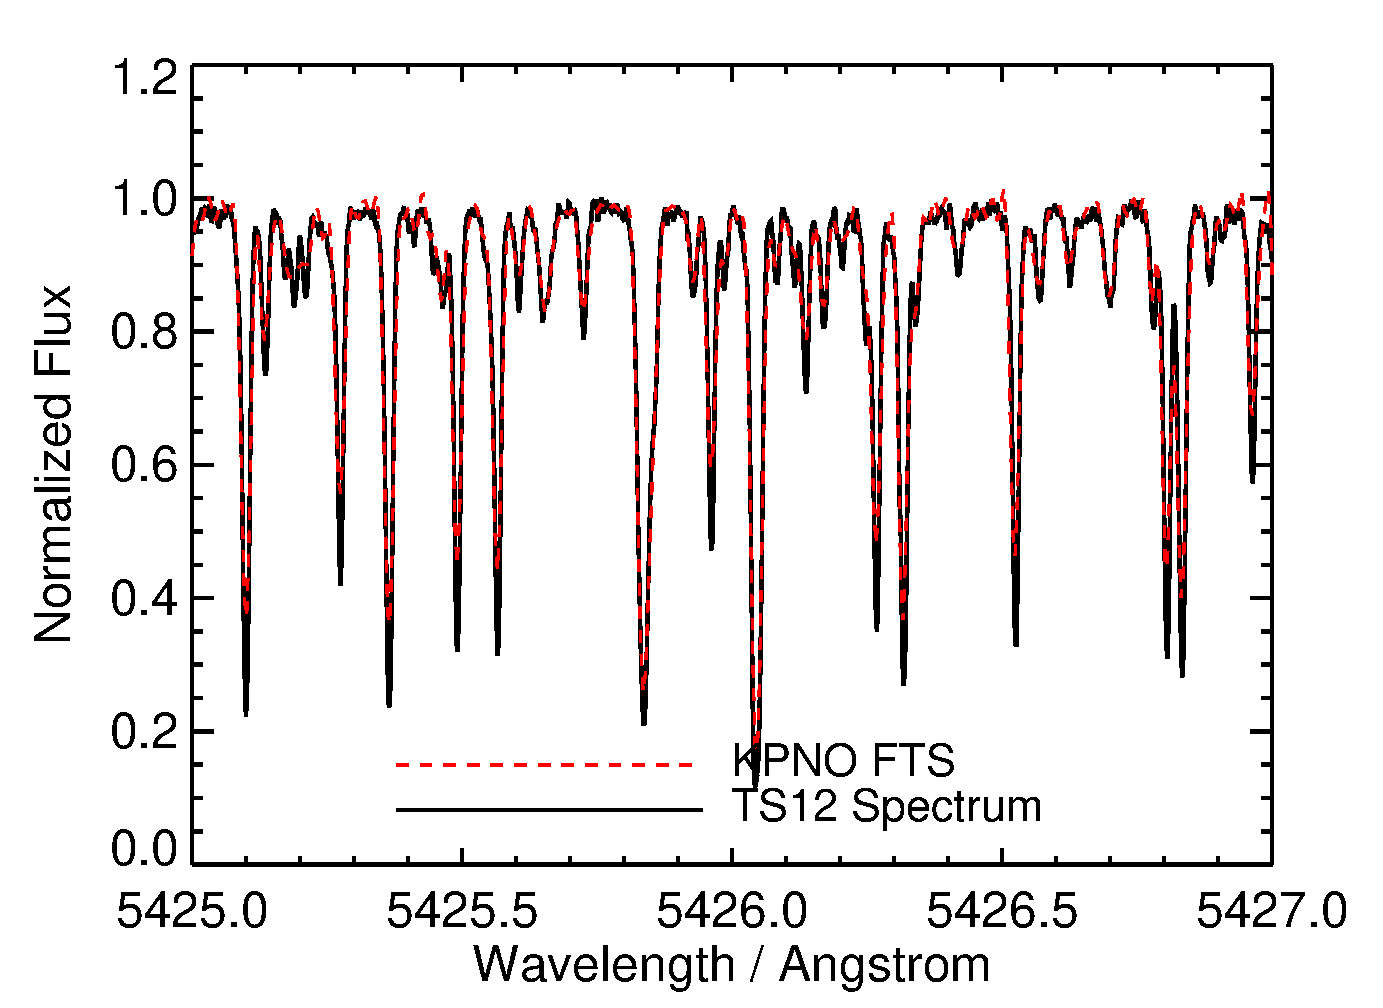
\includegraphics[angle=0.,scale=0.33]{het/chunk_5425A_original_sclrem.eps}
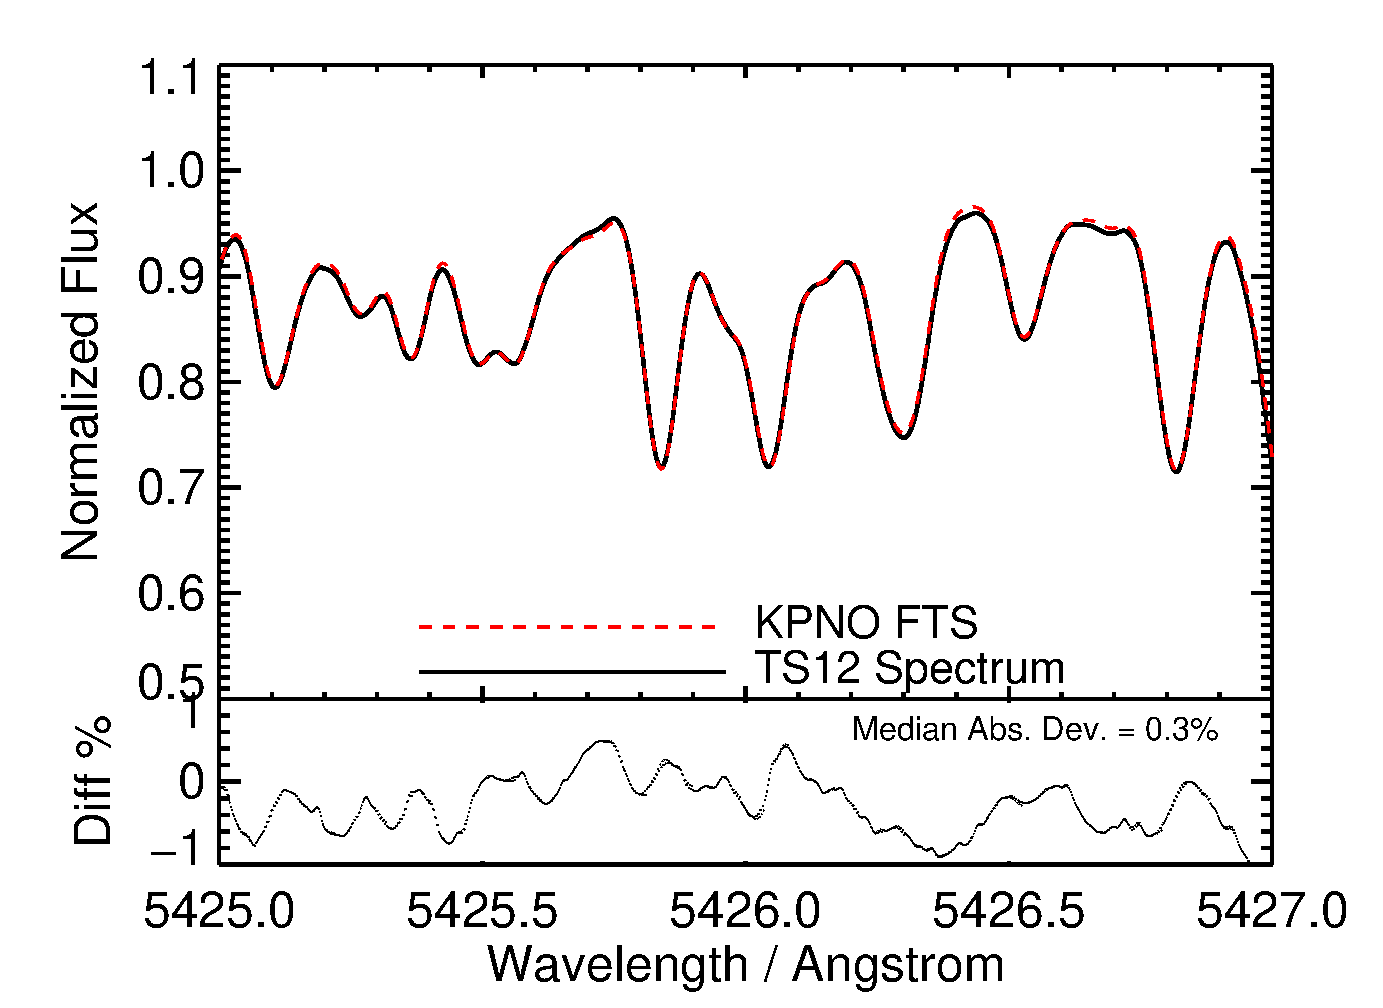
\includegraphics[angle=0.,scale=0.33]{het/chunk_5425A_60k_gaus_sclrem_diff.eps}
\caption{Comparison of the Sandiford iodine cell KPNO FTS spectrum and
  the spectrum taken with TS12. \textbf{Left:} Comparison of the two
  spectra in their native resolutions (both about
  $400,000$--$500,000$). \textbf{Right:} Comparison of the two spectra
  convolved down to about $60,000$ resolution, which is the resolution
  of typical iodine observations or radial velocity observations
  (star$+$iodine). Bottom panel shows the residuals in percentage of
  the TS12 spectrum minus the KPNO spectrum, with a median absolute
  deviation of 0.3\%.
  \label{fig:ts12}}
\end{figure*}
%----------------------------------------------------------------


%----------------------------------------------------------------
% Figure: TS12 spectrum vs. KPNO FTS scan, 60k, all, with residuals
\begin{figure}[!th]
\centering
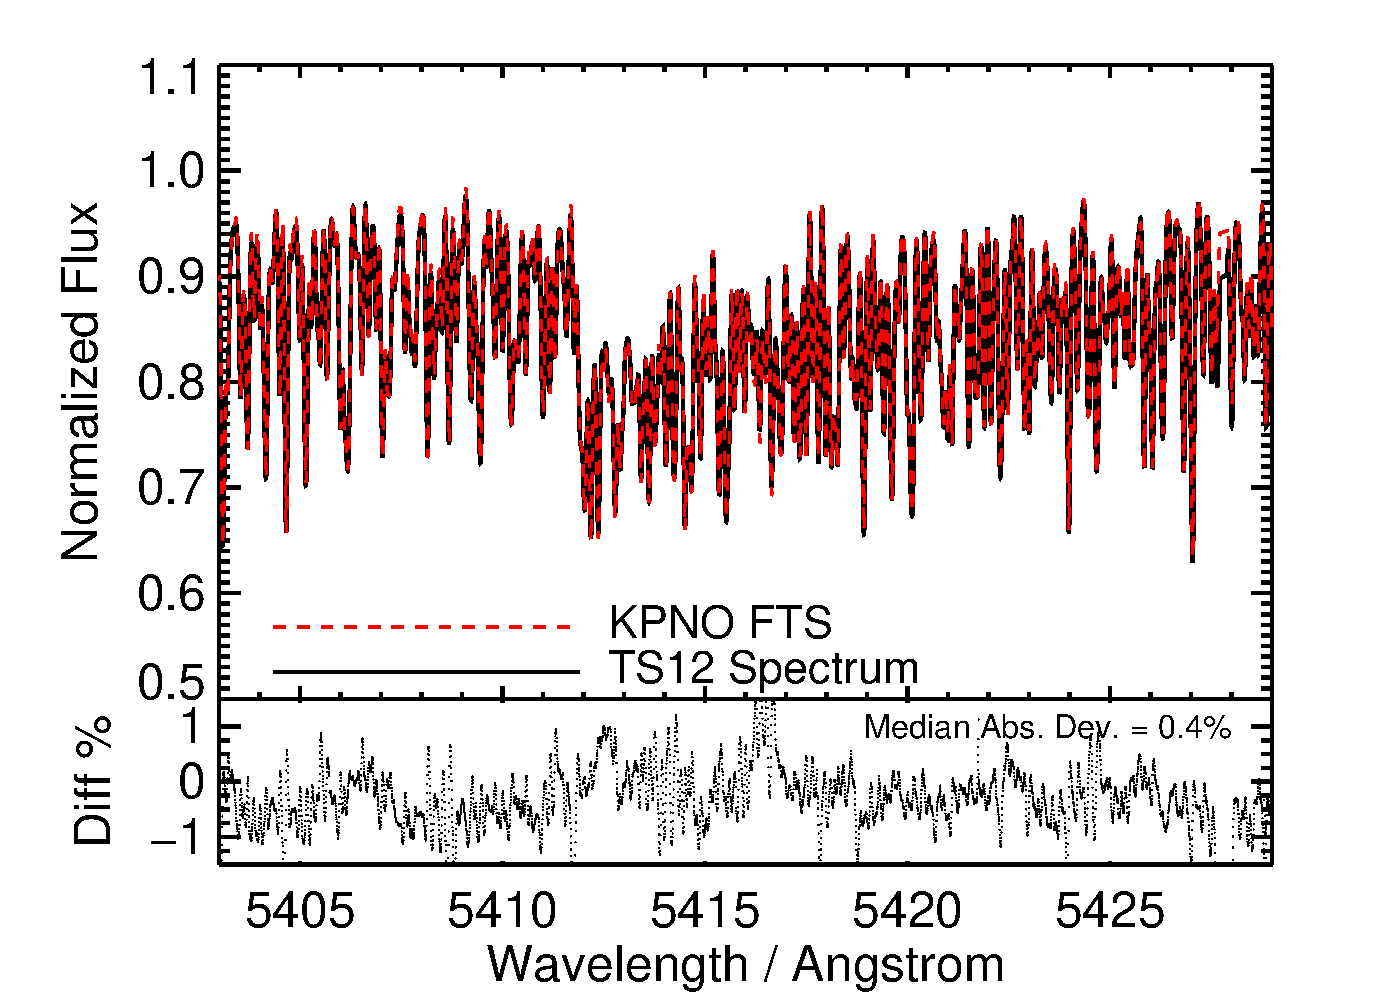
\includegraphics[angle=0.,scale=0.45]{het/all_60k_gaus_sclrem_diff.eps}
\caption{The same as the right panel of Figure~\ref{fig:ts12}, the
KPNO spectrum and the TS12 spectrum for the Sandiford cell both at
$60,000$, but for the entire $\sim$30\AA\ TS12 spectrum available. 
  \label{fig:60k_all}}
\end{figure}
%----------------------------------------------------------------


After demonstrated that we can use TS12 spectrum to validate FTS
scans, we performed our second TS12 run with the \het\ cell (and the
2.7m cell and the MINERVA cell). For
the 2.7m cell, its TS12 spectrum matches very well to its FTS atlas,
again (together with the 2.1m cell data from 2013) proving that TS12
is an appropriate tool for validating FTS atlases. For the HET/HRS
iodine cell, the results are very informative:

(1) Assuming that the \het\ cell temperature control was reliable
during our TS12 run (Phillip MacQueen from McDonald Observatory, who
built the cell and its enclosure, was at the TS12 run to set it up),
then temperature change on the order of 5--10$\degree$C in iodine cell
should induce a visible change in the absorption spectrum (right panel
of Figure~\ref{het:fig:tempchange}). On the other hand, the
temperature of the iodine gas in the cell was not at its set
temperature of $70\degree$C during the NIST scan (left panel of
Figure~\ref{het:fig:tempchange}). This could explain the difference
between \het\ cell's NIST scan and the KPNO scan. The NIST scan
appears to have stayed at higher than $70\degree$C the entire time
(one hypothesis is that the gas on the light path was heated up by the
ultra-luminous continuum lamp, while the glass container, which the
temperature probe was monitoring, stayed cool). The \keck\ cell was
also scanned at three different temperatures (50, 60, and
70$\degree$C) at KPNO in 1993, and there are also visible differences
between these three sets of scans.


%----------------------------------------------------------------
% HET cell spectral changes vs. temperature changes effects in TS12 and NIST scan
% plot made by
% ~/ExoPlanet-2010-2011/HET-HRS-IP/05-Iodine_FTS_investigation/compare_fts/explore_temp_change.pro and saved therein
\begin{figure}
\centering
\subfloat{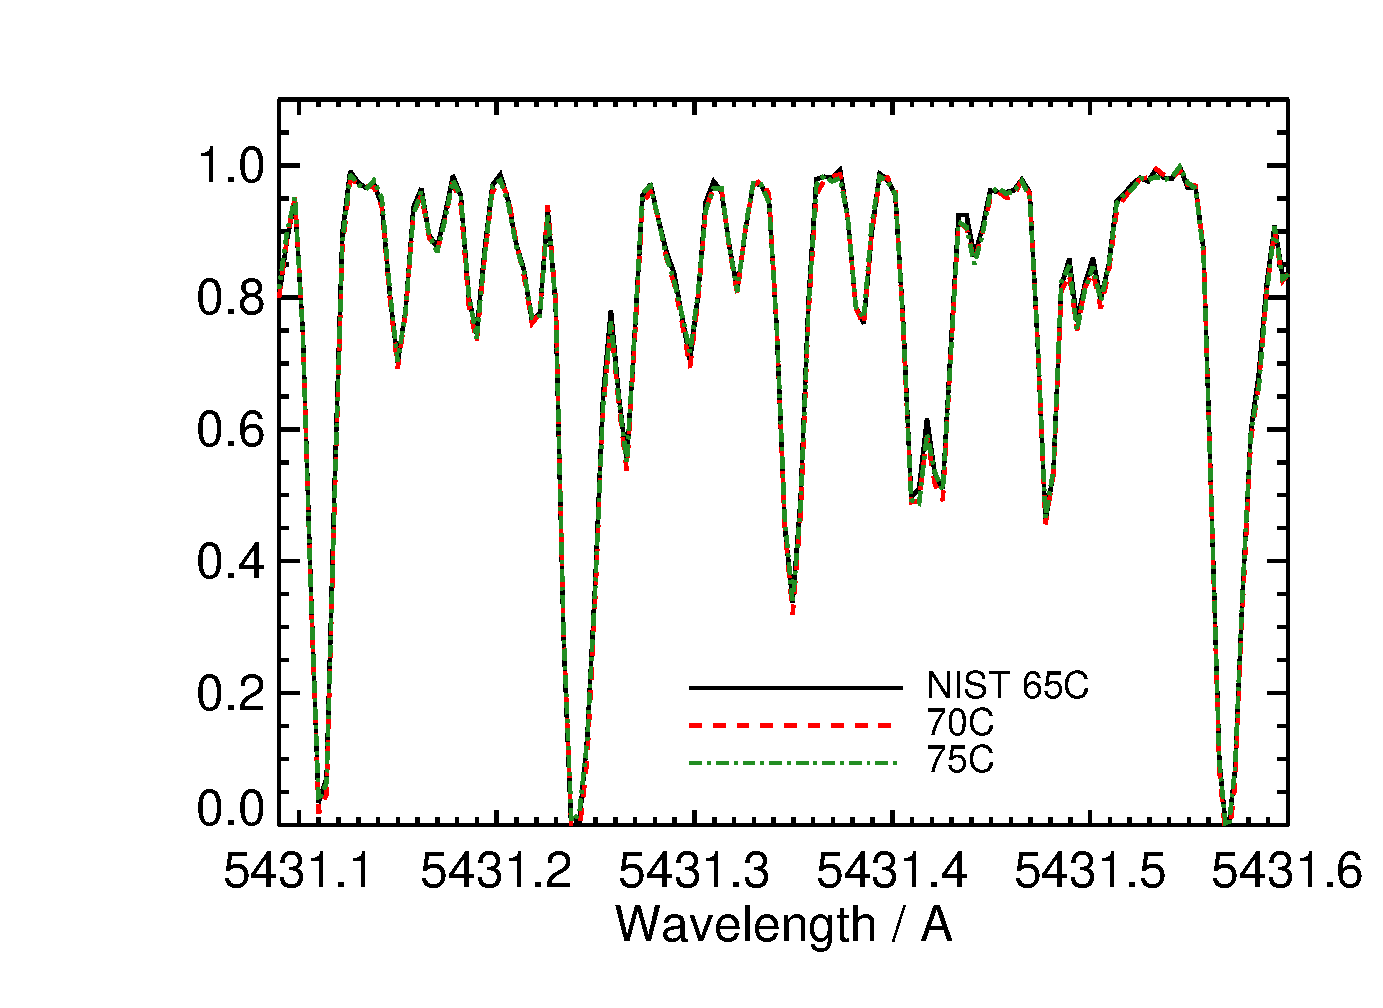
\includegraphics[scale=0.32]{het/nist_temp_change.eps}}
\subfloat{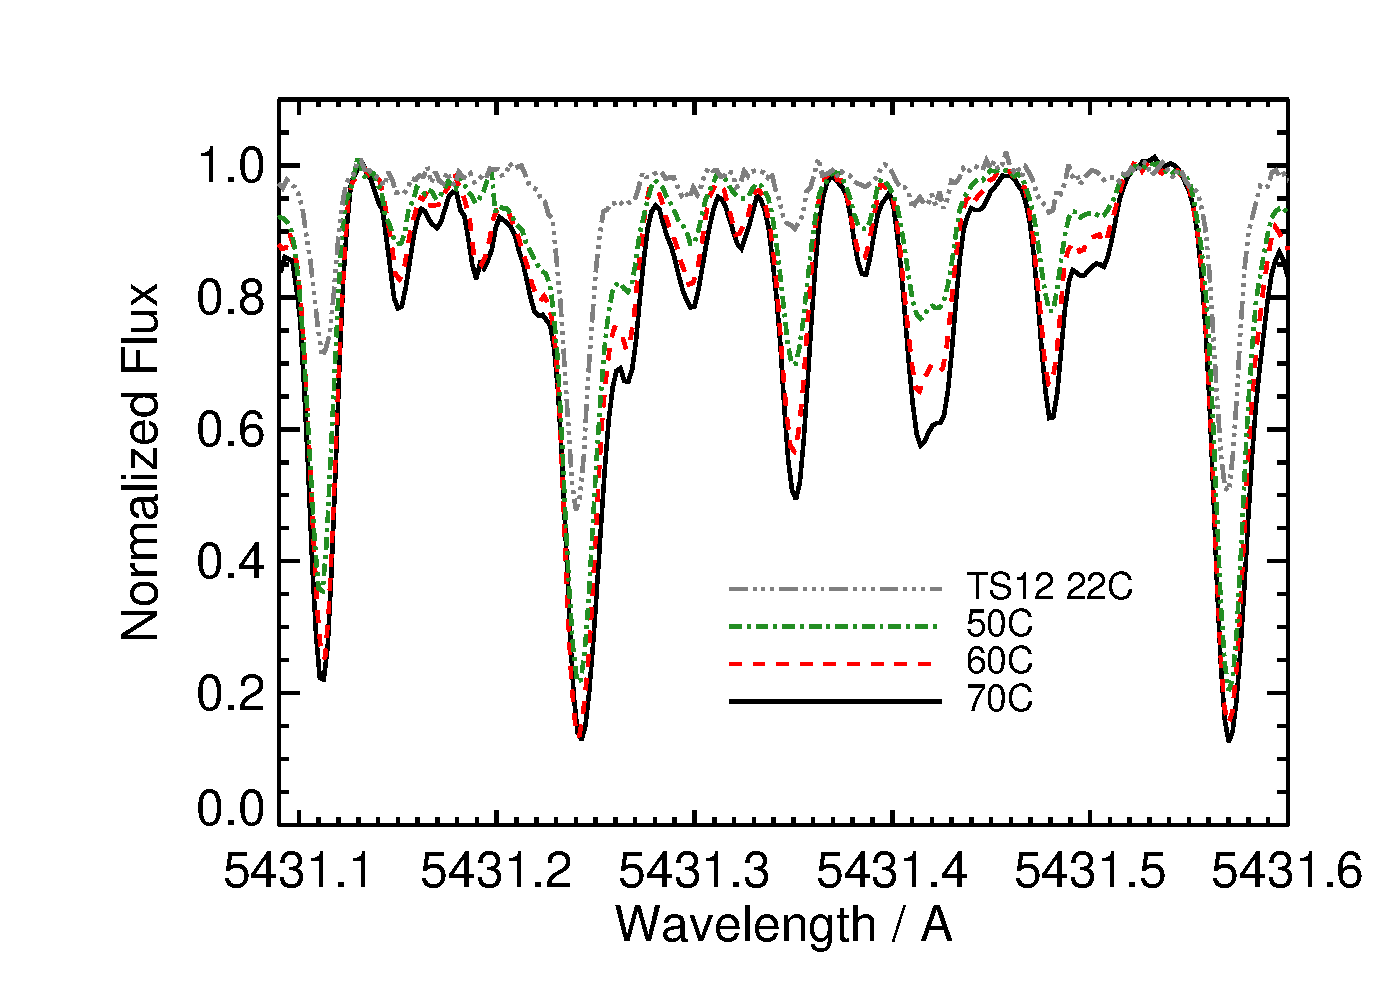
\includegraphics[scale=0.32]{het/ts12_temp_change.eps}}
\caption{{\bf Left:} \het\ cell NIST FTS scan at three different
temperatures. {\bf Right:} \het\ cell TS12 spectra at four different
temperatures for the same wavelength region, which, unlike the NIST
scans, shows significant difference when the temperature of the cell
changes by 10$\degree$C.
\label{het:fig:tempchange}}
\end{figure}
%----------------------------------------------------------------



(2) The TS12 spectrum at $70\degree$C matches better with the more
recent but potentially problematic NIST FTS atlas
(Figure~\ref{het:fig:hetts12}). This is completely unexpected and
contradicts with the assumptions and/or conclusions we lay out in
finding (1). The TS12 spectrum also does not match the FTS scan well
enough given the high SNR nature of both. Perhaps neither TS12 or the
NIST scan was at $70\degree$C. Or, perhaps the amount of iodine vapor
was somehow different. 


%----------------------------------------------------------------
% HET/HRS cell, TS12 vs KPNO vs NIST
% plot from ~/TS12/match_fts/figure/, made by plotcomp.pro
% grabbed from ~/ExoPlanet-2010-2011/Professional_Development/201402-NESSF/renewal/proposal/
\begin{figure}
\centering
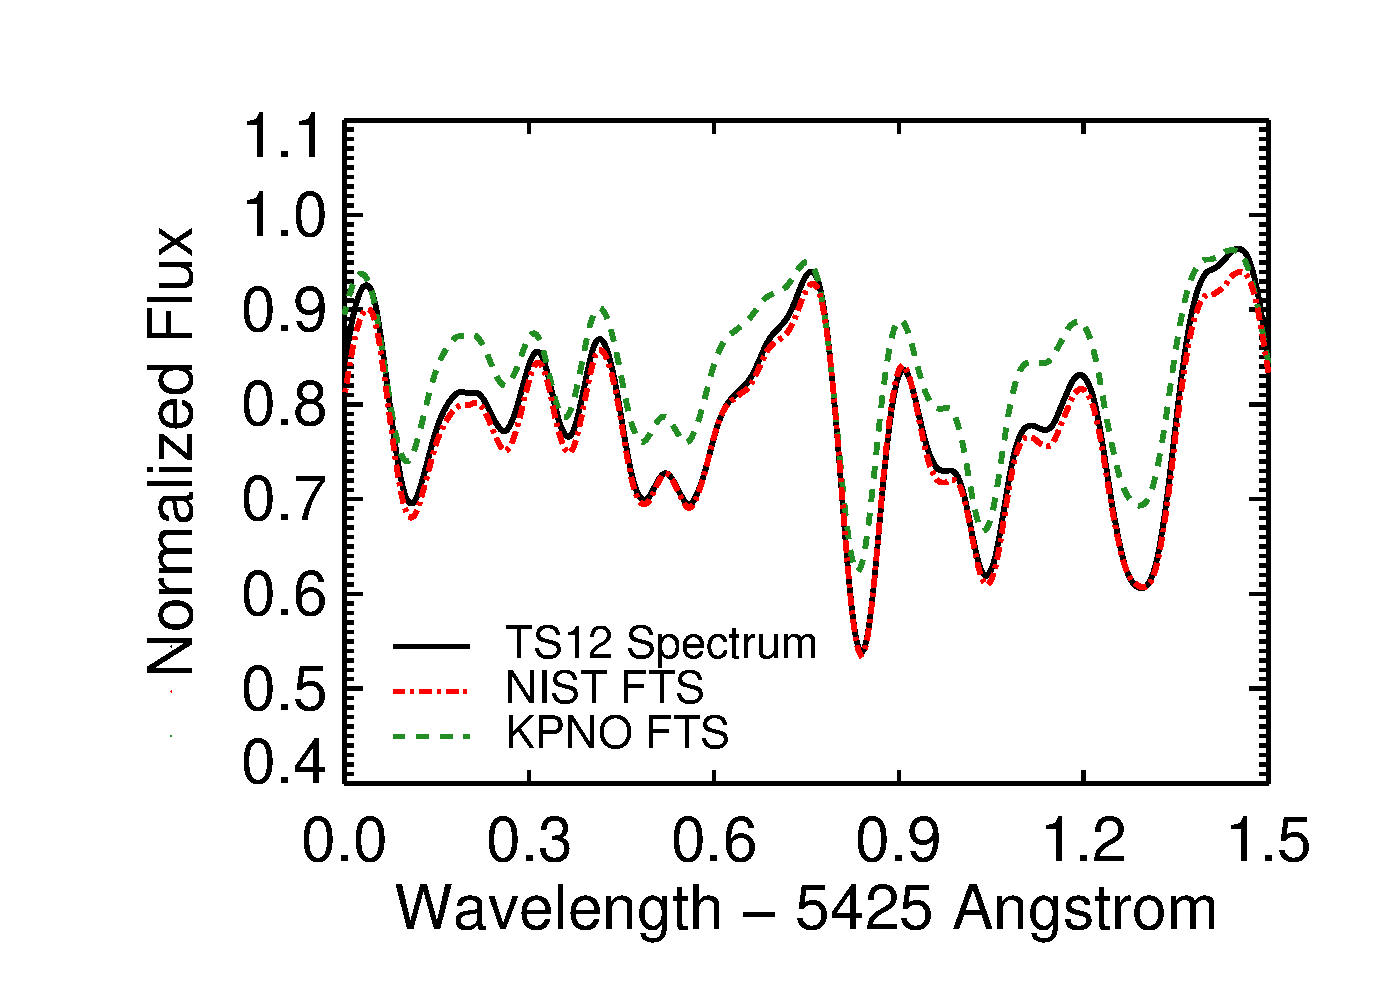
\includegraphics[scale=0.5]{het/het70_comp.eps}
\caption{TS12 spectrum (black solid line) vs.\ NIST FTS (red
  dotted-dashed) vs.\ KPNO FTS (green dashed) for the \het\ iodine
  cell at 70$\degree$C, all convolved down to a resolution of R $=$
  60k (the same as a typical \het\ observation) for comparison
  purposes. The TS12 spectrum matches the NIST FTS better, having
  deeper lines compared to the original KPNO FTS. The remaining
  difference between NIST FTS and the TS12 spectrum might be due to
  differences in cell temperatures or other changes with the cell. 
\label{het:fig:hetts12}}
\end{figure}
%----------------------------------------------------------------

These results prompted us to resolve for a second route to try to break
the tie: using synthetic iodine absorption spectra, which is described
in the next subsection.


%%%%%%%%%%%%%%%%%%%%%%%%%%%%%%%%%%%%%%%%%%%%%%%%%%%%%%%%%%%%%%%%%%%%%%%%%%%%%%%%%%%%%%%%%%%%%%%%%%%%
\subsection{Measuring iodine cell temperatures using synthetic Iodine spectra}

Using the TS12 spectra, we found that the temperature of the iodine
gas in the cell might not be the same one reported by the temperature
controller. However, we still could not break the tie between the KPNO
scan and the NIST scan for \het\ cell: the KPNO scan provides a better
fit to real observed data, but the TS12 spectrum shows us that the
NIST scan looks closer to the ``truth'' as defined by TS12. Nor did we
understand why the KPNO scan for the \keck\ cell works the best for
\het\ data.

To answer these questions, we have found\footnote{We are deeply
  grateful for Iouli Gordon for introducing IodineSpec5 to me
  during my visit at CfA.} a second venue that provides
reliable, ultra-high resolution, and wavelength calibrated iodine
atlas -- a theoretical code that computes synthetic iodine
transmission spectrum (at any specified temperature) based on both
physics and empirical calibrations (IodineSpec5;
\citealt{iodinespec5}). We emailed the authors and obtained the code,
which only runs on Windows machines. The direct output of the code
contains arrays of wave numbers and ``opacity'' ($\alpha$) for user-specified
iodine isotope mix (for our purposes we only add $^{127}I_2$),
temperature, wave number range, and line broadening kernel parameter
(we chose thermal/Gaussian). To use the output of IodineSpec5 to fit
an actual iodine absorption spectrum, there are two parameters:
gas temperature and a constant which scales with iodine molecule
column density, which we simply refer to as the column density hereafter.

Quickly comparing the NIST scan with the IodineSpec5 models reveals
that the NIST scan seems to be around 110$\degree$C, mostly based on
visually examining the line ratios
(Figure~\ref{het:fig:nisteyeball}). However, the synthetic iodine
spectrum and the FTS scans have different broadening kernels. In order
to ``fit'' the NIST scan with the synthetic spectra at various
temperatures, we convolved the NIST scan with a single Gaussian kernel
with $\sigma=0.0078$ (roughly at $R=$ 200,000 to try to match the
\keck\ cell KPNO scan for comparison and illustration
purposes). Except for the \keck\ scan, we did the same to lower the
resolution of other FTS scans or TS12 spectra when using IodineSpec5
to find out their temperatures. There are three four parameters in our
fit: temperature, column density, resolution ($\sigma$ for the single
Gaussian kernel to convolve the synthetic spectrum with), and a
wavelength shift. We first optimized the column density, $\sigma$, and
the wavelength shift while fixing the temperature (using L-M
least-$\chi^2$ fitter using {\tt mpfitfun} package in IDL), and then
we compare the goodness of fit of each model at different temperatures
to determine which temperature best describes the FTS scan or TS12
spectrum. The reason for this two-step optimization is because we have
to generate the IodineSpec5 model spectra on a discrete temperature
grid.


%----------------------------------------------------------------
% HET/HRS cell, IodineSpec5 2 temperatures vs. NIST, and KPNO
% plot from ~/ExoPlanet-2010-2011/IodineSpec5/, made by plots_general.pro
\begin{figure}
\centering
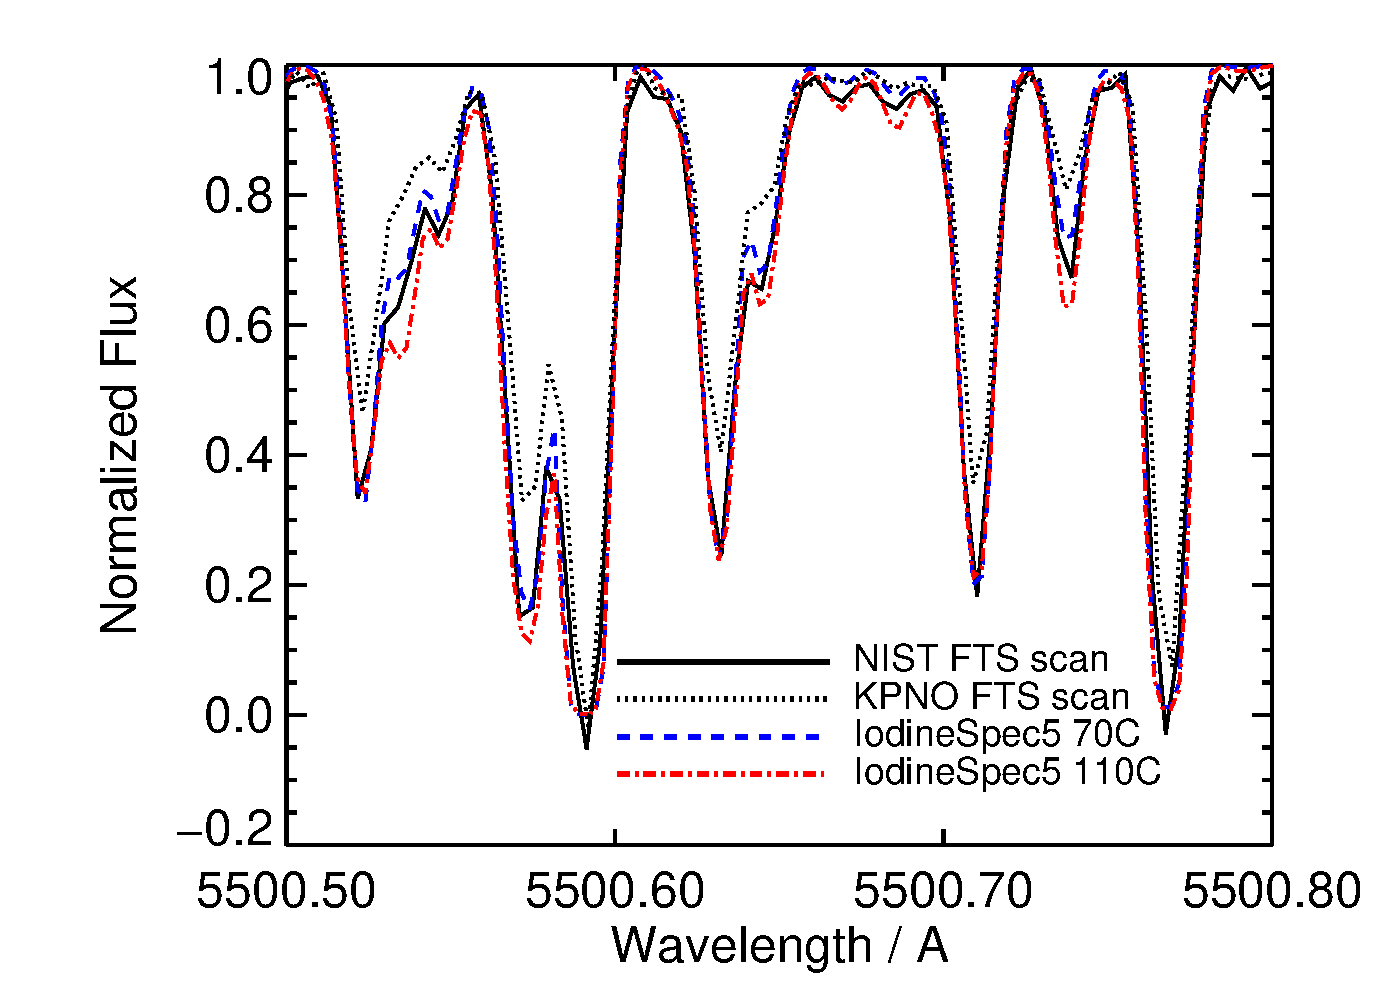
\includegraphics[scale=0.5]{het/HET_NIST_temp.eps}
\caption{NIST FTS (black solid lines) and KPNO FTS (black dotted
lines) compared with theoretically computed iodine lines at
70$\degree$C (blue dashed) and 150$\degree$C (red dotted-dashed). All
spectra are at their original resolution. There are two free
parameters for the theoretical lines: temperature and iodine column
density. For this plot, we optimized the iodine column density for the
theoretical lines at both temperatures to try to match the NIST FTS. As
illustrated, neither temperature can produce a good match, and the
best temperature is around 110$\degree$C. Note that the
theoretical lines and the NIST FTS have different broadening
kernels. The NIST and KPNO FTS scans probably differ in both optical
depth and cell temperature.
\label{het:fig:nisteyeball}}
\end{figure}
%----------------------------------------------------------------

We first fitted the \keck\ cell KPNO FTS scan, whose temperature is
known (50$\degree$C) and reliable. We also know that this FTS scan is
probably very trust-worthy since \keck\ iodine atlas fits the data
very well, as described in the previous subsection. Choosing a region
where it contains temperature-sensitive lines, we found the best-fit
temperature for the \keck\ KPNO scan is 55$\degree$C, although
synthetic spectra ranging from 40-70$\degree$C all fit the data
almost equally well and they are hard to distinguish (column density
and temperature are highly degenerate parameters). 

We then fitted the NIST scan, which has the highest SNR and
resolution among all FTS scans or TS12 spectra (we also have a rough
idea about its temperature). The results are shown in
Figure~\ref{het:fit:nistfit}, where the top panel shows the best-fit
models at different temperatures, and the bottom panel compares the
NIST scan with its the best-fit model at 110$\degree$C, the KPNO scan,
and the \keck\ cell KPNO scan. 


%----------------------------------------------------------------
% NIST scan fit by IodineSpec5 and comparison with FTS
% plot made by
% ~/ExoPlanet-2010-2011/HET-HRS-IP/05-Iodine_FTS_investigation/compare_fts/fit_temp_change.pro and saved therein
\begin{figure}
\centering
\subfloat{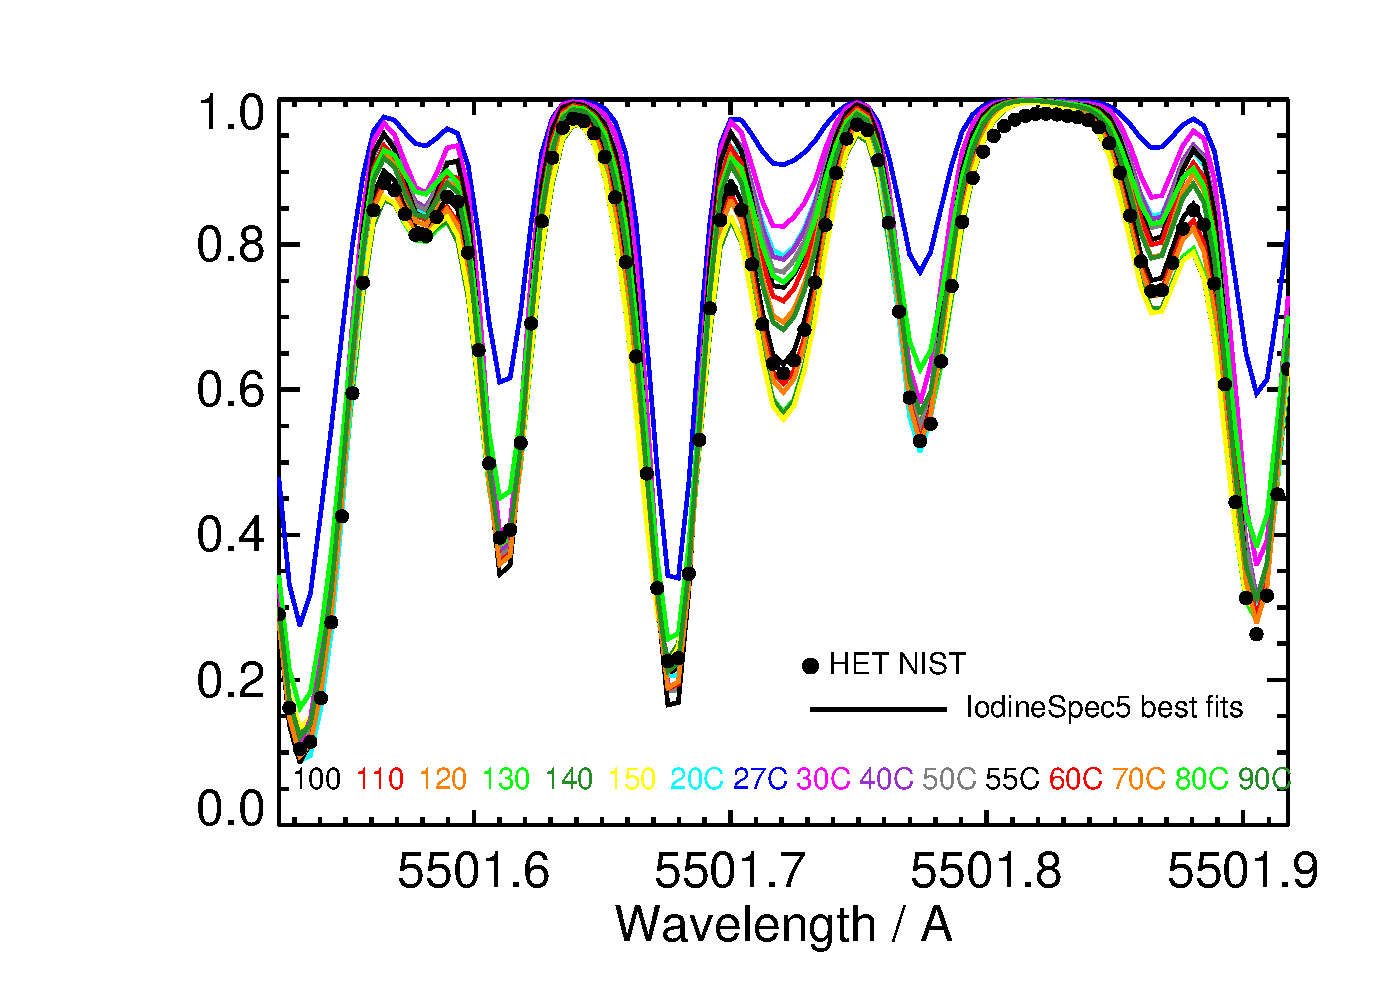
\includegraphics[scale=0.5]{het/hetnist_bestfits.eps}}\
\subfloat{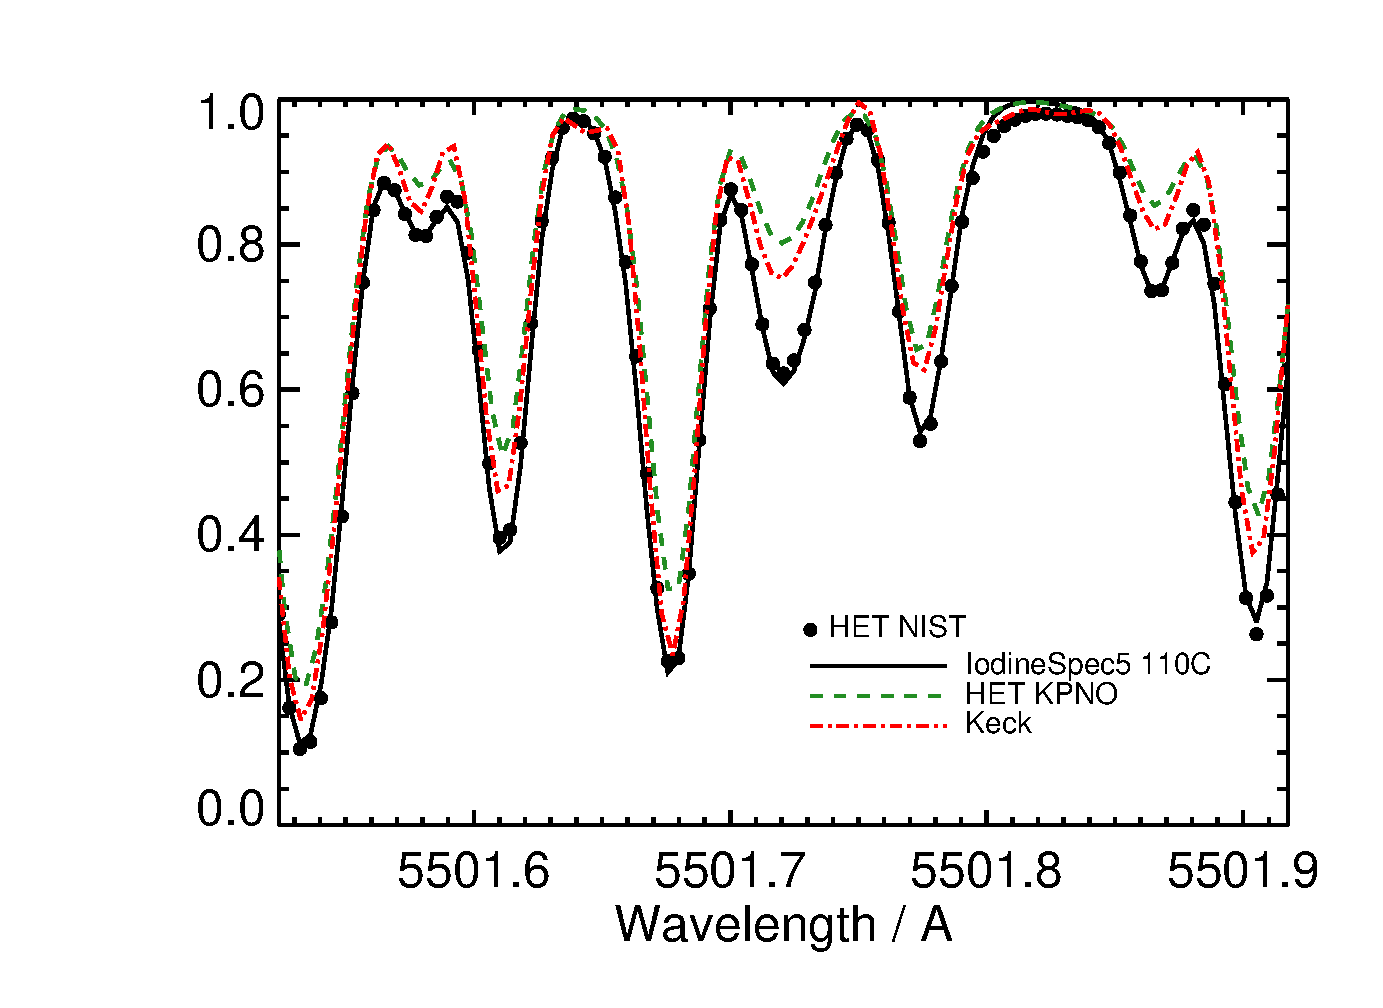
\includegraphics[scale=0.5]{het/hetnist_compWithOthers.eps}}
\caption{{\bf Top:} Fitting \het\ NIST scan (black dots; temperature
set at 70$\degree$C) with IodineSpec5 synthetic iodine lines at
various temperatures and column densities. {\bf Bottom:} The \het\
NIST scan (black dots) overplotted with the best-fit IodineSpec5 model
(black solid line; at 110$\degree$C) and the \het\ cell and \keck\ 
cell KPNO scans. All spectra in both panels are convolved down to a
resolution of 200,000 (roughly \keck\ KPNO FTS scan resolution) to
wash out the intrinsic IP difference between FTS scan (sinc function
IP) and the synthetic spectrum (only natural broadening IP models).
\label{het:fig:nistfit}}
\end{figure}
%----------------------------------------------------------------

When we tried to fit the \het\ KPNO scan, the high degeneracy between
column density and temperature hindered us from getting an accurate
estimate for the temperature. Models in 40-80$\degree$C appear to fit
equally well with varying column densities. However, only the fit at
$70\degree$C has the same column density as the best-fit value derived
from the NIST fit. We thus fixed the column
density in our fits for \het\ KPNO scan, and (unsurprisingly) the best-fit
temperature came out to be $70\degree$C. Therefore, we conclude that
the NIST scan was indeed at a different gas temperature, and the old
KPNO scan seems to be at the right temperature.

But how about the TS12 spectrum? Again, using the best-fit column
density derived from our NIST and KPNO fits, we estimated the
temperatures for the TS12 spectra (supposedly) at 50, 60, and
70$\degree$C. The best-fit temperature turns out to be 55$\degree$C
for claimed 50$\degree$C TS12 spectrum, 80$\degree$C for the
60$\degree$C one, and 100$\degree$C for the 70$\degree$C one. The
results fitting for the ``70$\degree$C'' TS12 spectrum are in
Figure~\ref{het:fig:ts12fit}.  


%----------------------------------------------------------------
% TS12 fit by IodineSpec5 and comparison with FTS
% plot made by
% ~/ExoPlanet-2010-2011/HET-HRS-IP/05-Iodine_FTS_investigation/compare_fts/fit_temp_change.pro and saved therein
\begin{figure}
\centering
\subfloat{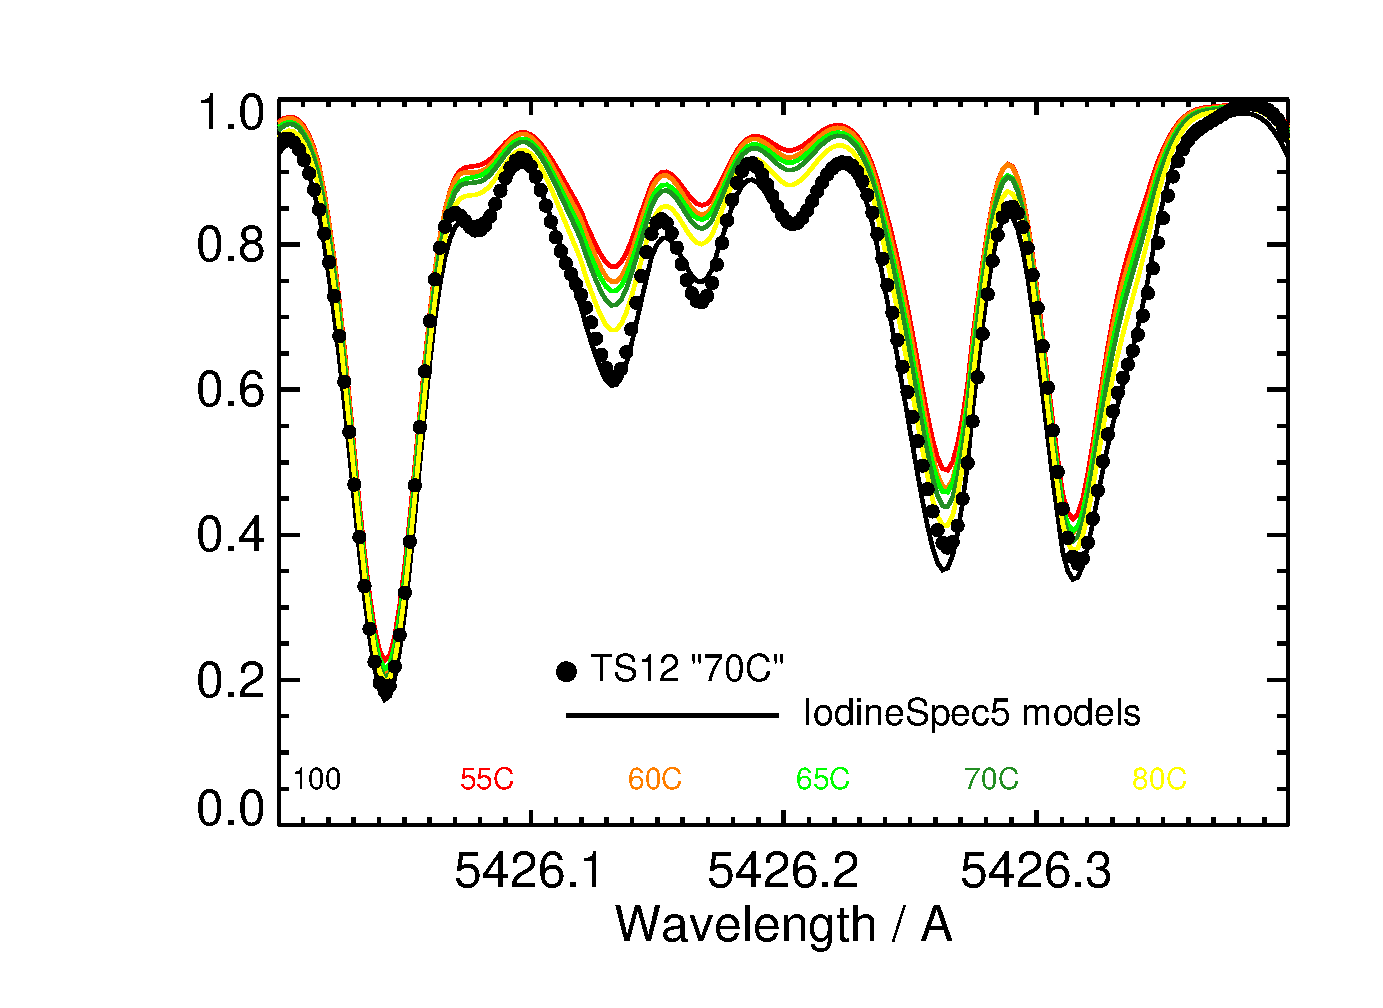
\includegraphics[scale=0.5]{het/ts12_70_bestfits.eps}}\
\subfloat{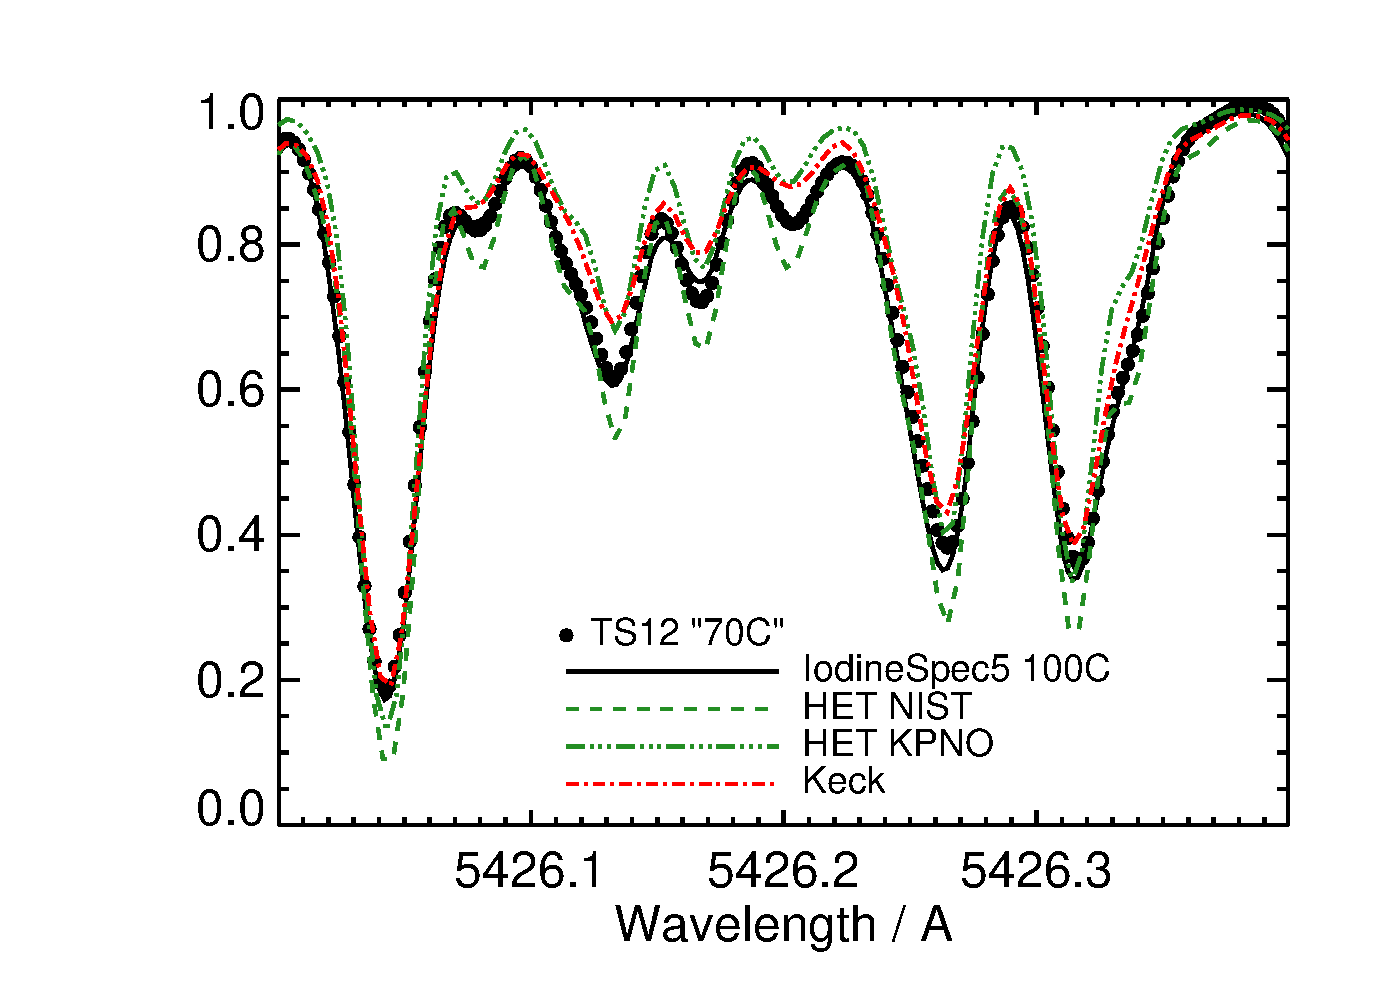
\includegraphics[scale=0.5]{het/ts12_70_compWithFTS.eps}}
\caption{{\bf Top:} Fitting the TS12 spectrum (temperature set at
70$\degree$C; black dots) with IodineSpec5 models, with fixed column
density derived from best fits using \het\ KPNO and NIST scans. {\bf
Bottom:} The best-fit temperature for the TS12 spectrum is about
100$\degree$C (black solid). It is clearly at a lower temperature than
the NIST scan (green dashed) but at a higher one than the KPNO one
(green dotted-dashed). Again, all spectra in both panels are convolved
down to $R=$ 200,000.
\label{het:fig:ts12fit}}
\end{figure}
%----------------------------------------------------------------

These findings on \het\ cell temperatures could explain the fits to
real data. If the \het\ cell was kept at a higher temperature (e.g.,
$\sim 100\degree$C) instead of $70\degree$C when it was in active use
for precise RV calibration (despite what the temperature control
reported), or if the actual temperature of the gas in the cell changes
over time, then the KPNO scan, which was done at $70\degree$C,
certainly cannot fit the observed data and provide precise
calibrations to measure RVs to the level of \keck, which has a precise
iodine atlas. Looking at the bottom panel of
Figure~\ref{het:fig:ts12fit}, it is not hard to imagine why the \keck\
cell scan provides the best fits to \het\ data
(Figure~\ref{fig:lampi2fit}) -- if the gas temperature is between 70
and 110$\degree$C during actual observations (and perhaps more often
closer to 70$\degree$C), then an iodine atlas which has line depths in
between the KPNO and the NIST scans would provide a better fit, which
the \keck\ scan happens to satisfy.

We believe that the difference between the iodine atlas and reality as
a result of temperature changes or differences is the dominant factor
behind \het's under-performance in RV precision compared with
\keck. We outline potential solutions to improve the RV precision of
\het\ archival data and our recommendations for the new HRS in the
next section.


%%%%%%%%%%%%%%%%%%%%%%%%%%%%%%%%%%%%%%%%%%%%%%%%%%%%%%%%%%%%%%%%%%%%%%%%%%%%%%
%\section{The Investigation on Modal Noise}
 

 
%%%%%%%%%%%%%%%%%%%%%%%%%%%%%%%%%%%%%%%%%%%%%%%%%%%%%%%%%%%%%%%%%%%%%%%%%%%%%%
\section{Conclusion and Future Work}\label{het:sec:conclusion}
 
To summarize, we think that two of the major drivers behind \het's RV
systematic errors are {\em temperature issues with the iodine
cell (or inaccurate iodine atlas which fails to capture such changes)
and inaccurate modeling of the IPs}. 

Overall, the \het\ spectra exhibit more changes than the \keck\
spectra, which probably makes it harder to model and leads to its
large RV systematic error (Figure~\ref{het:fig:chunkvary}). These
variations may be due to temperature changes in the cell or
spectrograph changes such as IP or focus changes. Precise Doppler
spectroscopy requires great care to minimize any changes in the iodine
cell and spectrograph performance. For example, standard CPS \keck\
observations are preceded with a series of procedures which ensures
that (1) the spectrograph is very well focused and (2) the wavelength
solution for the CCD chip stays roughly the same, i.e., the ThAr lines
always land on the same pixels. \het\ does not perform these
procedures, to the best of our knowledge.

%----------------------------------------------------------------
% Chunk pixel flux variation comparison between Keck and HET
% plot made by
% ~/ExoPlanet-2010-2011/HET-HRS-IP/05-Iodine_FTS_investigation/chunk_variation/chunk_vary.pro
% and plot_chunk_vary.pro and saved therein
\begin{figure}
\centering
\subfloat{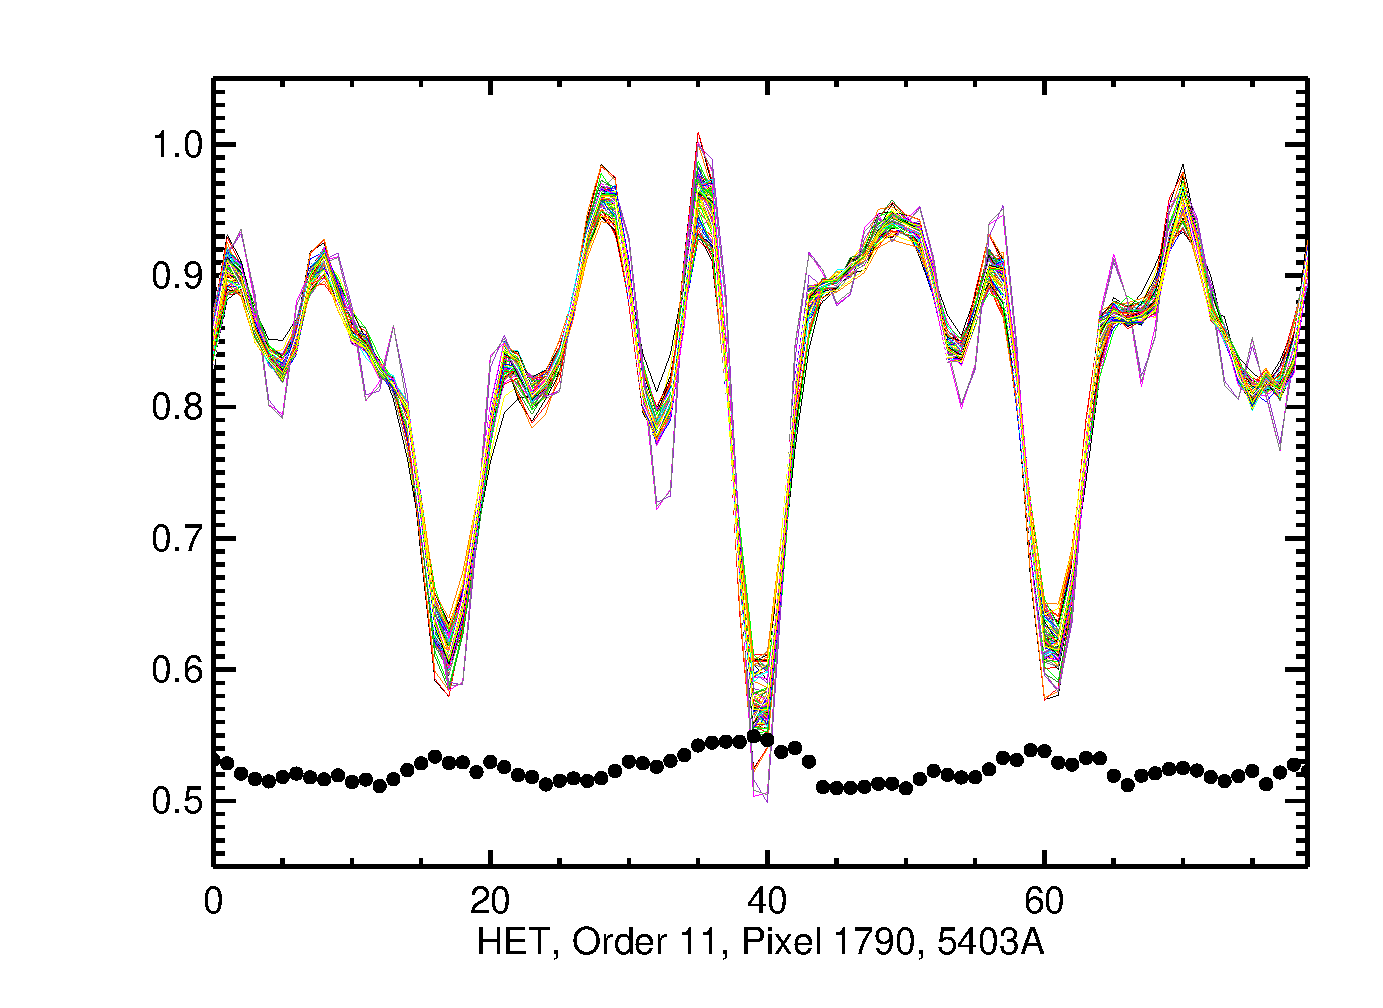
\includegraphics[scale=0.35]{het/het_chunk_variation.eps}}
\subfloat{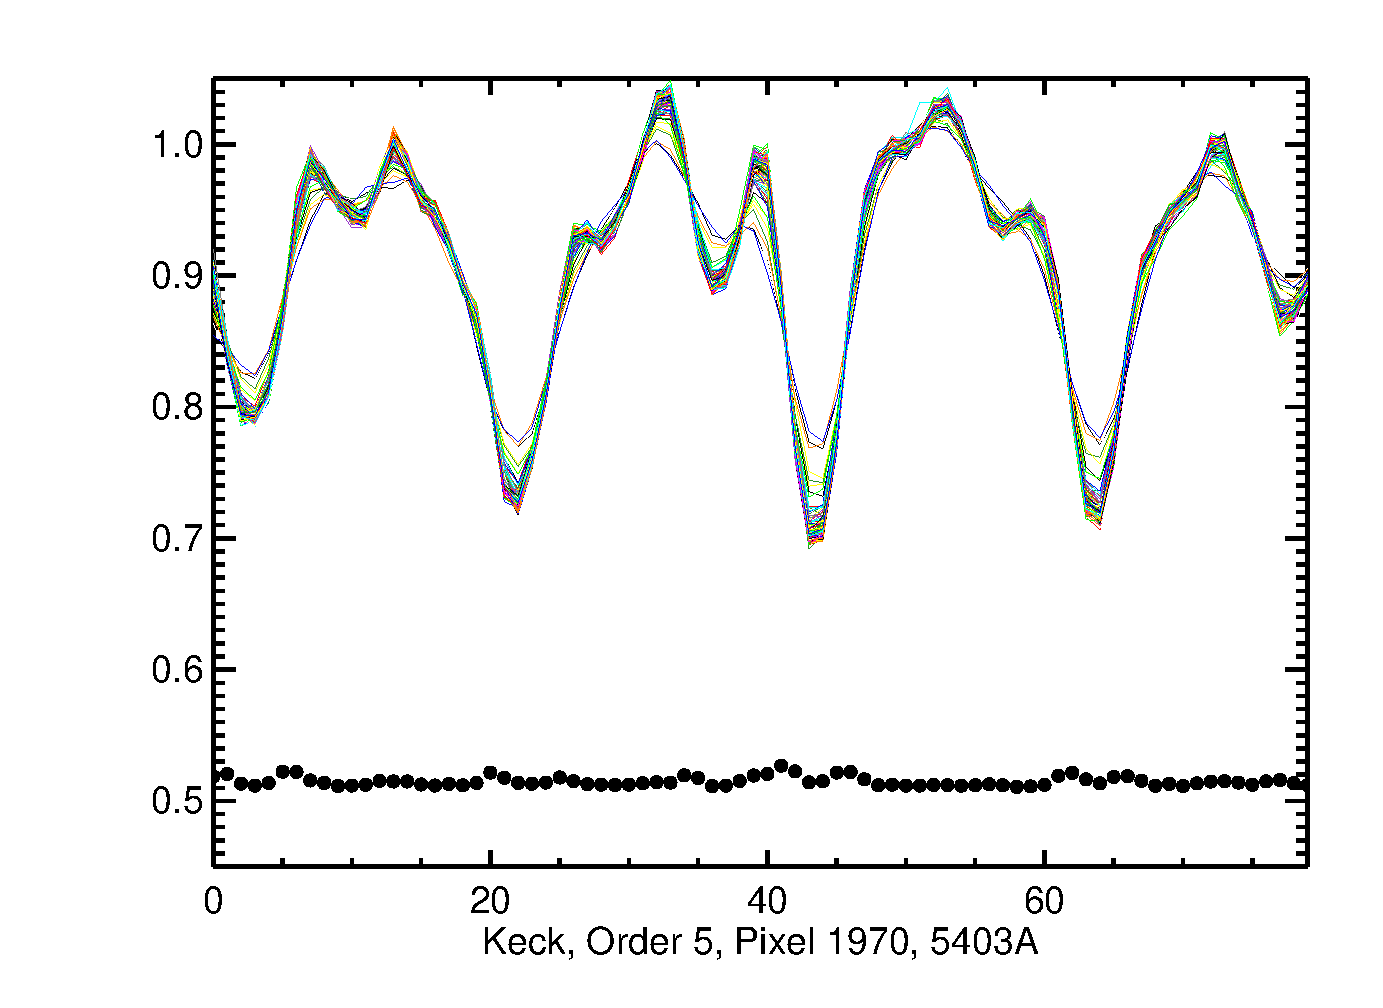
\includegraphics[scale=0.35]{het/keck_chunk_variation.eps}}\
\subfloat{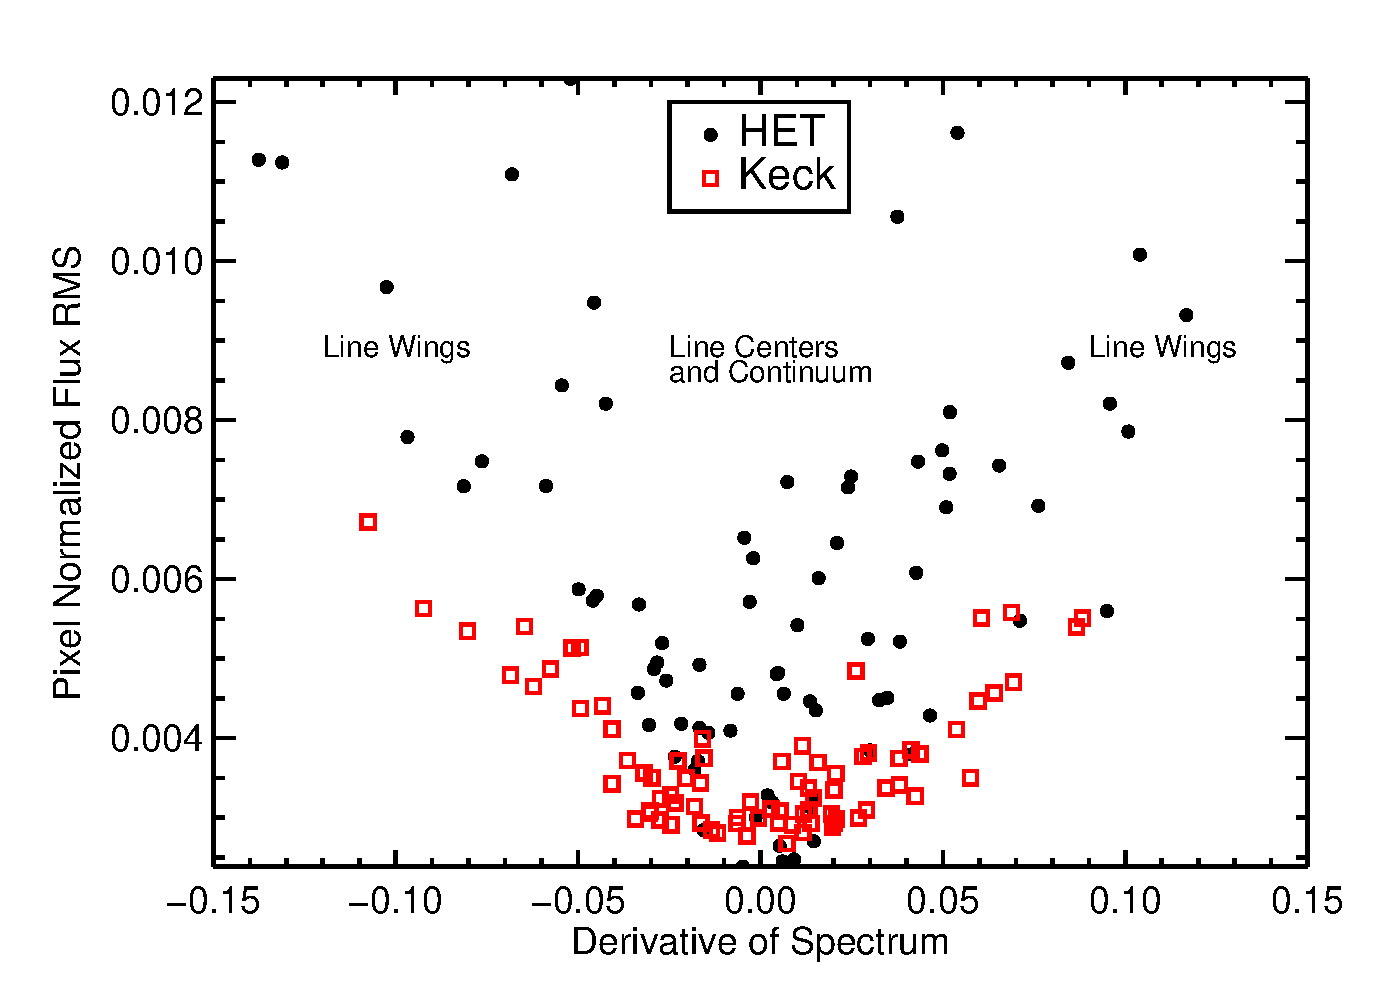
\includegraphics[scale=0.35]{het/line_spec_rms_keck_het.eps}}
\caption{Comparison between the amounts of variation in a spectral
chunk in $\sim 500$ \het\ and \keck\ lamp iodine observations,
respectively. The top two panels show the overplotted spectra in this
chunk, shifted and normalized so that the spectral lines match (using
cross correlation and interpolation; normalized using total counts in
this chunk). The black dots in each of the two top panels are the RMS
values of the normalized counts in each pixel, multiplied by 4 and
added by 0.5 for illustration purposes. The \het\ spectra exhibit
significantly more variation than the \keck\ spectra, and we discuss
potential reasons in Section~\ref{het:sec:conclusion}. The bottom
panel is ploting the pixel counts RMS as a function of the derivative
of the spectrum, which shows that the \het\ spectra have more
variation in both line centers/continuum and line wings than \keck.
\label{het:fig:chunkvary}}
\end{figure}
%----------------------------------------------------------------

Our adventure in improving the RV precision of \het, though incomplete
and sometimes inconclusive so far, have taught us several important
lessons for iodine-calibrated precise RV work:

\begin{itemize}
  \item The IP functional forms for fiber-fed spectrographs probably
differ quite significantly from slit-fed ones, and it is important to
find a good IP function which not only describes the IP well but also
has good convergence properties for the forward modeling.
fitter. Initial guesses on IP parameters could play an important role.
  \item The iodine atlas provided by FTS scans should not be taken for
granted as the ``ground truth''. There are challenges with FTS
measurements and data reduction for measuring absorption spectrum with
such a big spectral span. The cell can also change over time, nulling
any old FTS scans. Echelle spectrograph with hyper resolution like the
TS12 arm on the Tull Spectrograph is very helpful for validating
iodine atlas or checking cell quality.
  \item It is vital to stabilize the cell to a desired temperature
precicely and accurately, probably at least to $\pm$10$\degree$C or
even better at higher temperatures. Theoretical code computing iodine
lines such as IodineSpec5 is helpful for diagnosing problems with
iodine cells. One can imagine that this can also be helpful in
identifying permanent cell change like the one experienced by the
Lick/Hamilton cell, which compromised the usefulness of the
spectrograph for precise RV work fatally.
\end{itemize}

Looking forward, there are several things which can help solving the
mystery and hopefully eventually leading to an improvement in the RV
precision of \het:

{\bf (1) Determining cell temperature before extracting RVs} for each
observation. It is probably valuable to obtain FTS scans of the \het\
cell at various temperatures and interpolate between them to make a
finer model grids of iodine atlases at different
temperatures. Floating the temperature as a free parameter in RV
extraction is also an option, but the degeneracy it introduces will be
detrimental to the RV precision. Therefore, a better route is to use
the temperature-sensitive regions among the iodine spectrum to
determine the cell temperature first, then use the corresponding atlas
in the forward modeling process to determine RVs. Validating the
iodine atlas and temperature control
stability/reliability\footnote{The cell enclosure and temperature
controller for the \het\ used in our TS12 observations are the ones
for the new \het, which is troubling.} is crucial for the upgraded
\het.

{\bf (2) Finding a better IP function:} This can be first done through
fitting ThAr frames, and then tested via fitting B star $+$ iodine
frames, which would be a much easier task for observations with
pre-determined iodine cell temperature. We plan to continue to explore
possibilities with the modified Moffat function by adding
perturbations and providing good initial guesses.

{\bf (3) Examining the spectral data for modal noise or raw reduction
errors:} We have taken day time engineering data before the HET
shutdown/upgrade to test if modal noise is significant in \het\ data
in very high SNR regime. Although we have calculated that the number
of modes in the \het\ fiber is large enough that modal noise should
not be a concern, it would still be valuable to reduce and analyze
these data to prove this hypothesis.

More importantly, the upgraded \het\ has great promise in RV
precision, and carrying on these lessons is crucial for ensuring good
RV performance ($\sim$1~m/s) -- especially the lesson on iodine atlas
and cell temperatures. Chapter~\ref{chap:conclusion} has more
on the upgraded \het\ and related future work.




\chapter{Improving the Radial Velocity Precision of Keck/HIRES}\label{chap:keck}


%%%%%%%%%%%%%%%%%%%%%%%%%%%%%%%%%%%%%%%%%%%%%%%%%%%%%%%%%%%%%%%%%%%%%%%%%%%%%%%%
\section{Introduction and Background}

This is about Keck/HIRES.


%%%%%%%%%%%%%%%%%%%%%%%%%%%%%%%%%%%%%%%%%%%%%%%%%%%%%%%%%%%%%%%%%%%%%%%%%%%%%%%%
\section{Effects of Telluric Contamination and Remedies}\label{keck:sec:telluric}

% main text for the telluric section in keck.tex
%%%%%%%%%%%%%%%%%%%%%%%%%%%%%%%%%%%%%%%%%%%%%%%%%%%%%%%%%%%%%%%%%%%%%%%%%%%%
%%%%%%%%%%%%%%%%%%%%%%%%%%%%%%%%%%%%%%%%%%%%%%%%%%%%%%%%%%%%%%%%%%%%%%%%%%%%
\subsection{Introduction}\label{keck:telluric:intro}

The first exoplanets around main-sequence stars were discovered by the
radial velocity (RV) method, where precise Doppler spectroscopy
measures the wavelength shift of the host stars induced by the
gravitational pull of the planets \citep{1988ApJ...331..902C,
  1989Natur.339...38L, 1993ApJ...413..339H, 1995Natur.378..355M,
  1996ApJ...464L.153B}. Since then, the RV method has discovered
hundreds of planetary systems (see exoplanets.org; \citealt{eod2014})
and contributed to numerous confirmation and characterization of
exoplanets discovered by the transit method (e.g., for
\kepler\ follow-up observations; \citealt{Marcy2014}).

The current best RV precision is around 1~m/s \citep{eprv2015},
attainable via two wavelength calibration methods in the optical band:
ThAr lamp emission line calibration (e.g., ELODIE and HARPS;
\citealt{elodie, harps-s}; $\sim$400-690~nm) and iodine cell
absorption line calibration (e.g., Keck/HIRES and Magellan/PFS;
\citealt{butler1996, 2010SPIE.7735E..53C}; $\sim$500-620~nm). The
major obstacles for achieving a higher RV precision are: stellar
activity induced RV signals, instrumental effects, telluric
contamination, and limitation in data analysis \citep{eprv2015}.

Traditionally, telluric contamination is not considered as problematic
for precise RV in the optical. It is certainly a sever source of
spectral contamination and a bottleneck for achieving higher RV
precision in the near infra-red (NIR) region (e.g.,
\citealt{2010ApJ...713..410B}), where a large number of deep water and
methane lines reside. However, there is only a small wavelength
range in the optical that has deep telluric lines, and typically such
regions are simply thrown out for the purpose of precise RV analysis,
either by giving them zero weights in the cross correlation masks (for
ThAr calibrated spectra, e.g., \citealt{2002A&A...388..632P}) or
flagging them as bad pixels (for iodine calibrated spectra, e.g., for
Keck/HIRES).

Recently, the works by \cite{artigau2014} and \cite{cunha2014} have
characterized and mitigated the effects of telluric contamination in
the precise RV data taken by the ThAr-calibrated HARPS-S.
\cite{cunha2014} focuses on the issues with ``micro-telluric" lines
(shallow telluric absorption lines with $<1$-3\% depths), which are
recognized for the first time. \cite{cunha2014} fit and then divide
out the telluric lines in the observed spectra using synthetic
telluric spectra generated by the LBLRTM package (Line-By-Line
Radiative Transfer Model, \citealt{lblrtm}; with line lists from
HIgh-resolution TRANsmission molecular absorption database, or HITRAN,
\citealt{hitran2013}) and also TAPAS \citep{tapas}, which is a more
user-friendly but less flexible package wrapper using LBLRTM. They
concluded that the micro-tellurics have an impact (defined as RMS of
difference between RVs before and after micro-telluric removal) of
$\sim$10-20 cm/s for G stars observed with low to moderate air masses,
but the impact can be substantial in some cases to up to $\sim$0.5-1
m/s.

\cite{artigau2014} uses principal component analysis (PCA) to
empirically correct for telluric lines in HARPS-S data (both
micro-tellurics and the deep lines in the $\sim$630~nm region), and
combined PCA with rejection masking, they reduced the RV RMS by
$\sim$20~cm/s (and more significantly for the $\sim$630~nm
region). More recently, \cite{2016AAS...22713719S} characterized the
effects of telluric contamination and effectiveness of some typical
remedies (masking and modeling) for emission line-calibarated spectra
for the optical, broad optical (300-900~nm), and NIR. Their conclusion
for the optical region is similar to the results in \cite{artigau2014}
and \cite{cunha2014}.

This paper characterizes and corrects for the adverse effects of
telluric contamination under the context of iodine-calibrated precise
RV, especially for the micro-telluric lines. ZZZ We first describe our
methodology for characterizing the effects of tellurics in
Section~\ref{keck:telluric:method}, then... ZZZ


%----------------------------------------------------------------
% Plot showing micro-telluric lines
% made by ~/Exo../Keck../plots_general/spec_plot.pro
\begin{figure}
\includegraphics[scale=0.5]{telluric/tellurics_all.eps} 
\caption{Telluric lines in the iodine region are mostly shallow water
lines, with some moderately deep water lines near 5900\AA\ and very
deep oxygen lines near 6300\AA. The insert plot is showing the
pervasiveness of micro-telluric lines, i.e.~$\leq$1--3\% in depths.
\label{telluric:fig:telluric}}
\end{figure}
%----------------------------------------------------------------



%%%%%%%%%%%%%%%%%%%%%%%%%%%%%%%%%%%%%%%%%%%%%%%%%%%%%%%%%%%%%%%%%%%%%%%%%%%%
%%%%%%%%%%%%%%%%%%%%%%%%%%%%%%%%%%%%%%%%%%%%%%%%%%%%%%%%%%%%%%%%%%%%%%%%%%%%
\subsection{Impacts of Micro-tellurics on RV Precision}\label{keck:telluric:method}

% why Keck, why 185144 and 10700
To evaluate the impacts of micro-tellurics (referred to often simply
as ``tellurics'' below), we performed end-to-end simulation of \keck\
data and analysis process on RV standard stars in order to isolate
error sources. We use \keck\ data to for our study because Keck has
the highest RV precision among all iodine-calibrated spectrometers,
and it also has long observing baselines on a number of RV standard
stars. RV standard stars are bright and quite stars which do not host
known planets, and thus exhibit the smallest RV variation in both
short term and long term. Their data are often good diagnostic tools
for identifying RV systematics. For our study, we used and simulated
\keck\ RV spectra on two standard stars, $\sigma$ Draconis (HD 185144)
and $\tau$ Ceti (HD 10700), which are benchmark classics in precise RV
work.

% more on the two stars 
HD 185144 (spectral type G9V, per Simbad) has 712 \keck\ observations,
with RV RMS $=$ 2.57 m/s, and it has a relatively small barycentric
velocity (often referred to as the barycentric velocity correction, or
BC; see Chapter~\ref{chap:doppler}) span, $[-4.7,\ 4.6]$ km/s, because
it is near the north ecliptic pole. HD 10700 (spectral type G8.5V) has
623 observations, with RMS $=$ 3.05 m/s, and its BC span is $[-27.8,\
26.8]$ km/s. The RV RMS numbers quoted here come from reductions using
our version of CPS Doppler pipeline, and they are larger than the RMS
values from the most up-to-date CPS pipeline due to some recent
improvements in the CPS version. The most recent CPS inventory (as of
April 2016) also has a few new observations on these two stars.


%%%%%%%%%%%%%%%%%%%%%%%%%%%%%%%%%%%%%
\subsubsection{Methodology}\label{keck:telluric:method}

We simulated Keck observations on sig Dra and tau Ceti by using
synthetic stellar spectra of their respective spectral types (?) using
SME (ZZZ cite Valenti and Fischer). We simulated one spectrum for each
actual observed spectrum taken at Keck through the CPS programs. The
synthetic stellar spectra is multiplied with the iodine atlas to
create the standard iodine$+$ star RV observations. The multiplied
spectrum is then multiplied with the blaze function and convolved with
the observed spectral PSF, both derived from real observations for
each night. Poisson noise is added.

We then forward model the simulated spectra to extract RVs using the
CPS Keck code (ZZZ cite Johnson and Howard). We used the synthetic
stellar spectrum as the input stellar template. In reality, stellar
templates are derived from observed stellar spectra via deconvolution,
which would introduce additional errors. Using the same synthetic
stellar spectrum would eliminate such errors and isolate the problem
to telluric lines only.

We ran two sets of simulations: control and contaminated. In the
control, we only had stellar spectrum and iodine spectrum. In the
contaminated, we added in simulated telluric lines in the simulated
observed spectrum. The telluric lines were generated using TERRASPEC
(ZZZ cite Bender). We adopted the typical Mauna Kea atmospheric
condition (temperature and pressure profiles) and typical oxygen
column density (which in realiaty flucturate very little anyway). For
simplicity, we assumed the same water column density for every
observation, which is pwv$=1$mm, a little bit humid than a typical
Mauna Kea night (true? I think this is actually pretty typical). The
pair of simulated control and contaminated spectra have the same added
Poisson noise, and therefore any RV differences derived from these two
sets of simulation would reveal the net effect of telluric
contamination.


%%%%%%%%%%%%%%%%%%%%%%%%%%%%%%%%%%%%%
\subsubsection{Results}

%----------------------------------------------------------------
% Telluric effect, no photon noise
% plot made by ~/Exo.../Keck.../simulate.../msplot.pro
\begin{figure}
\subfloat{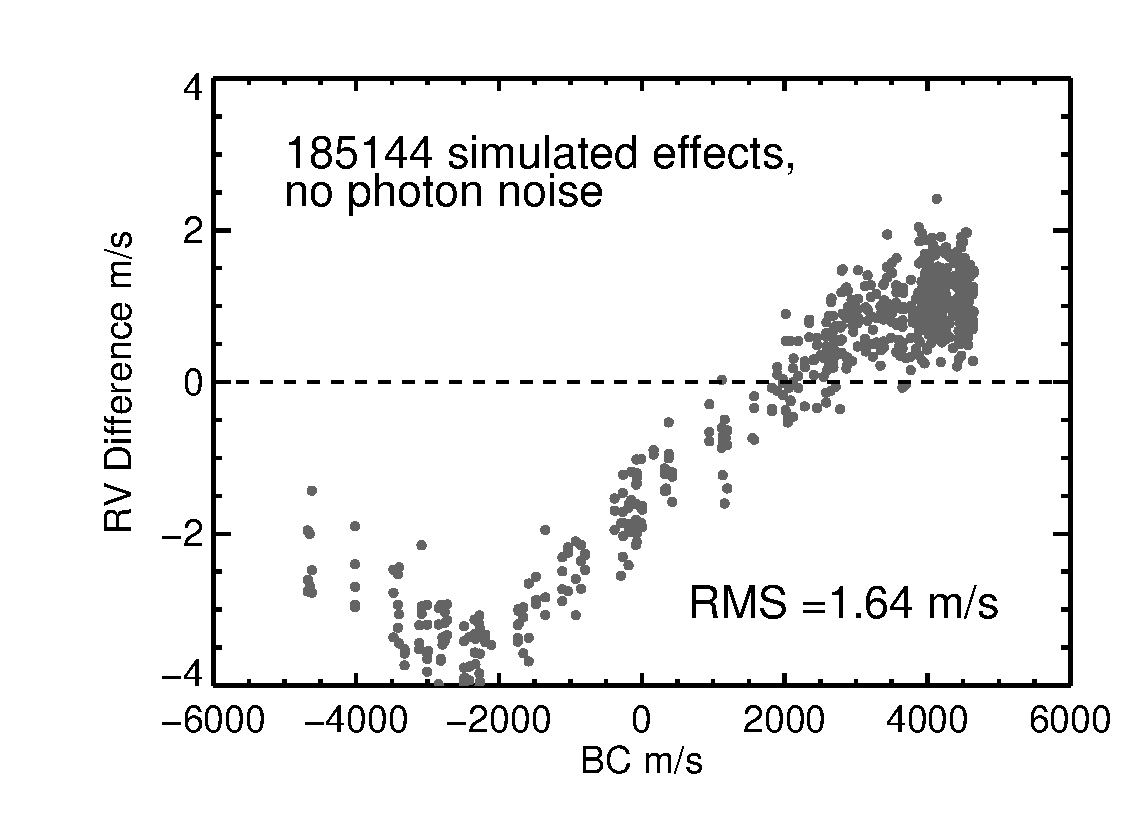
\includegraphics[scale=0.38]{telluric/185144-rv-bc-rja01-rjb01.eps}}\
\subfloat{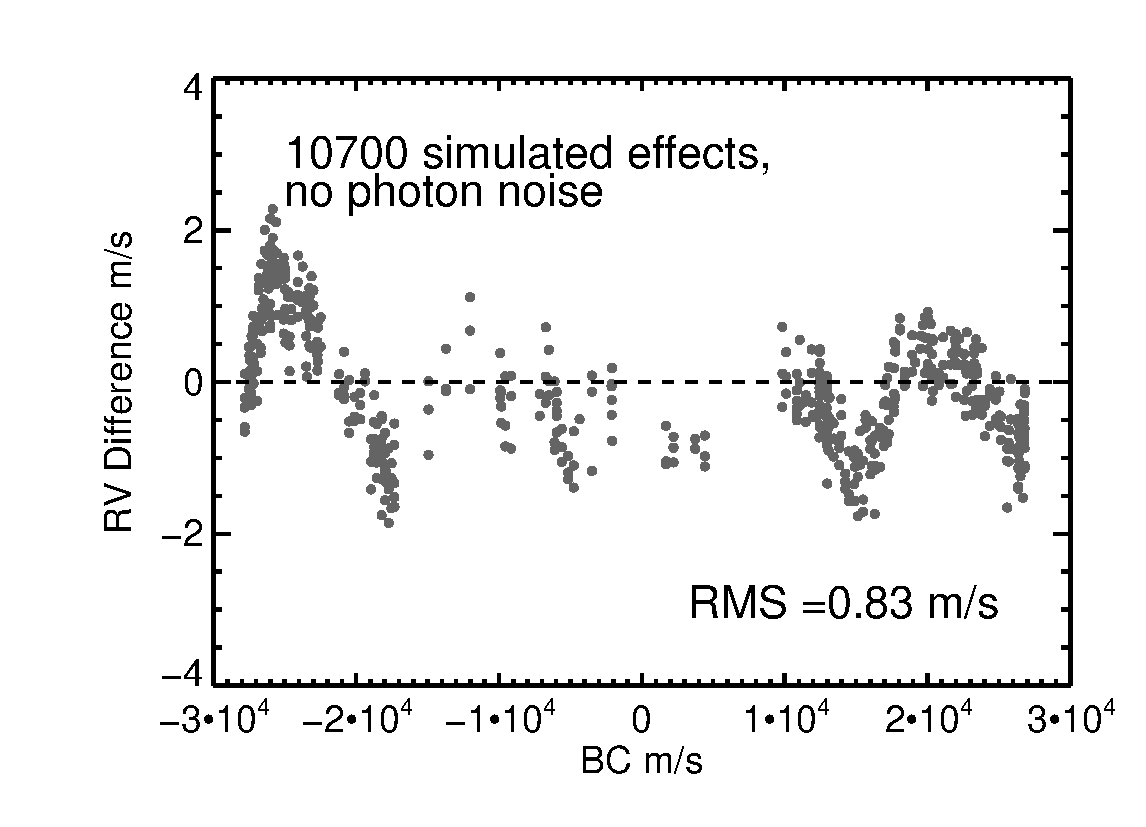
\includegraphics[scale=0.38]{telluric/10700-rv-bc-rja01-rjb01.eps}}\
\subfloat{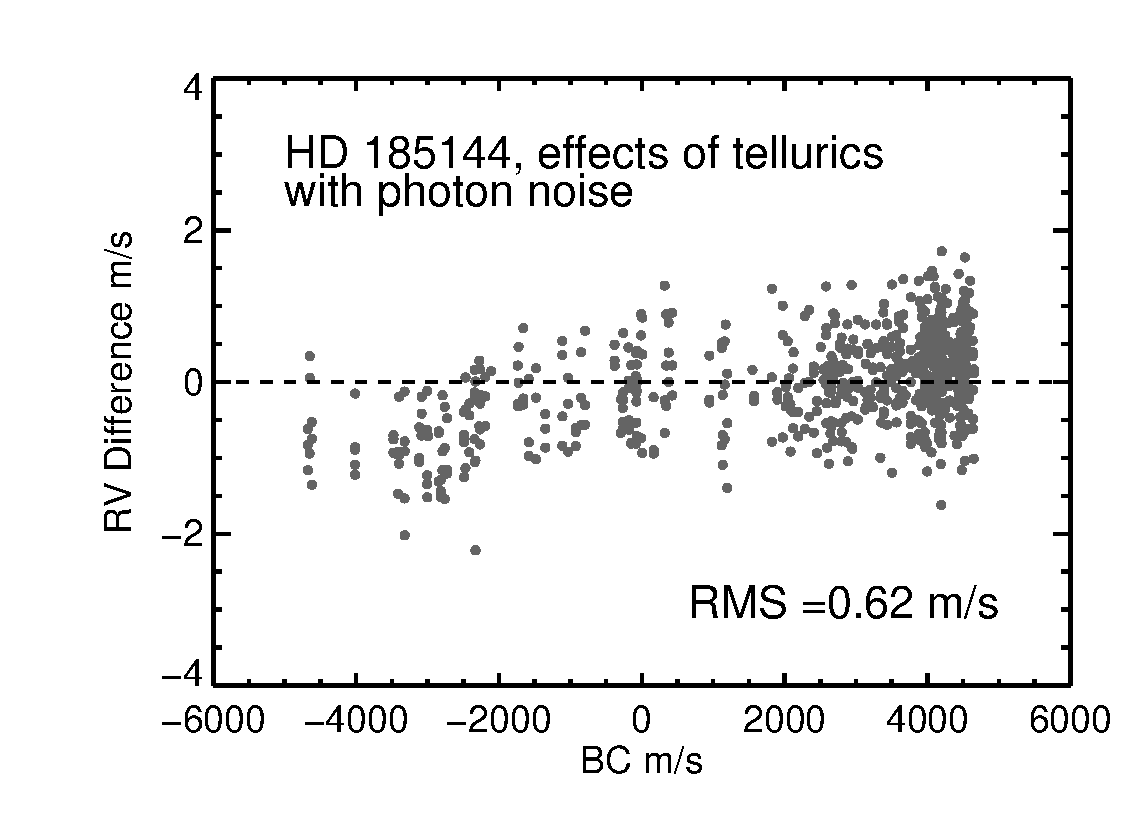
\includegraphics[scale=0.38]{telluric/185144-rv-bc-rjc01-rjd01.eps}}\
\subfloat{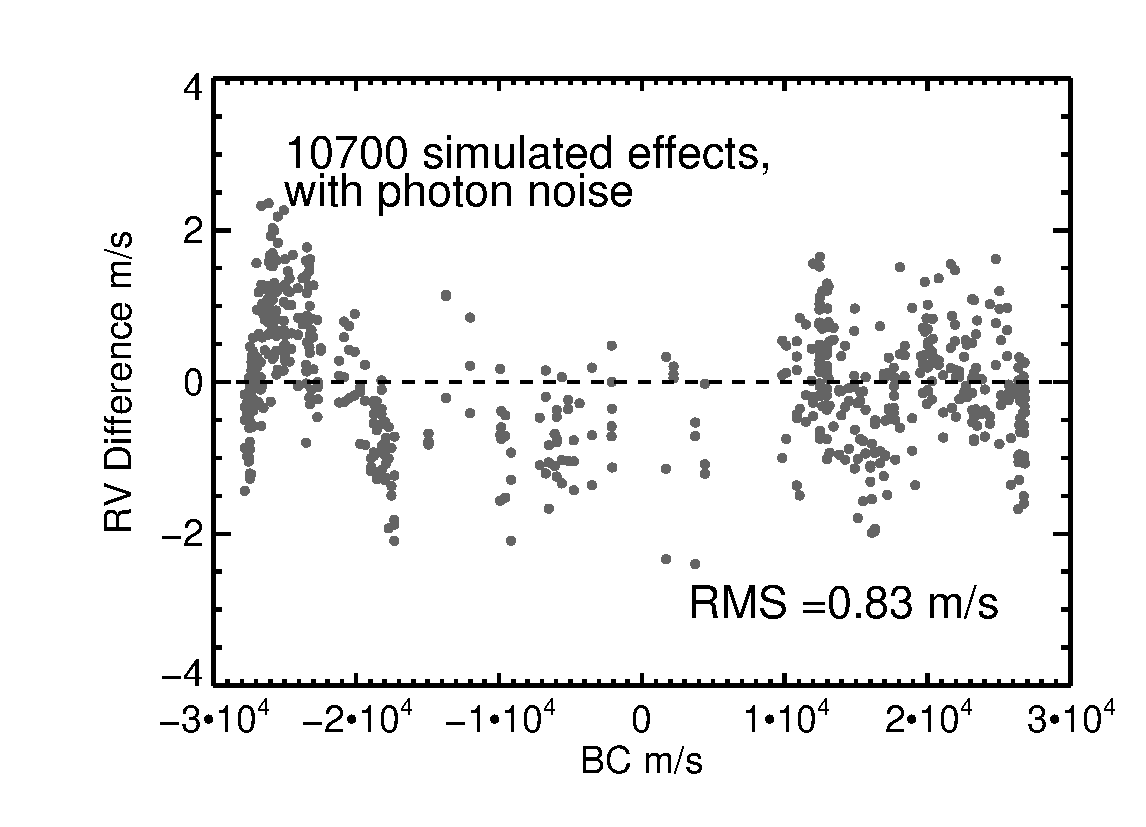
\includegraphics[scale=0.38]{telluric/10700-rv-bc-rjc01-rjd01.eps}}\
\subfloat{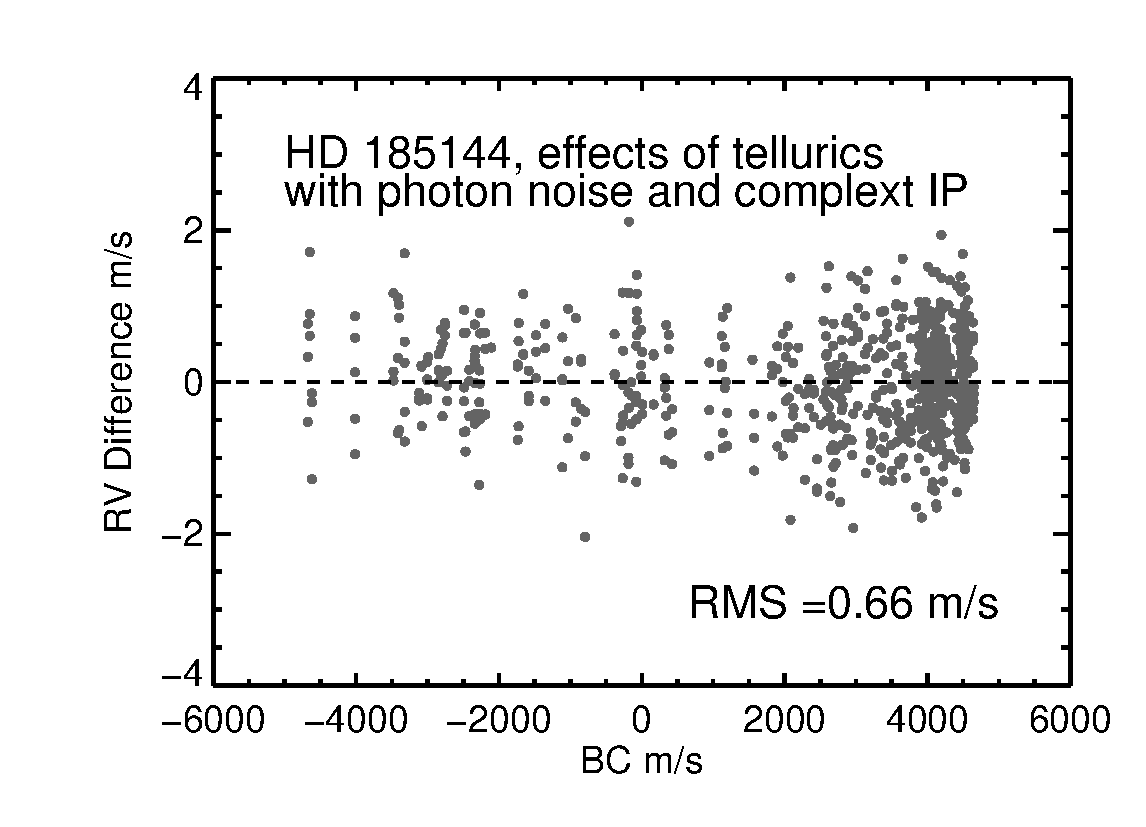
\includegraphics[scale=0.38]{telluric/185144-rv-bc-test0-test1.eps}}\
\subfloat{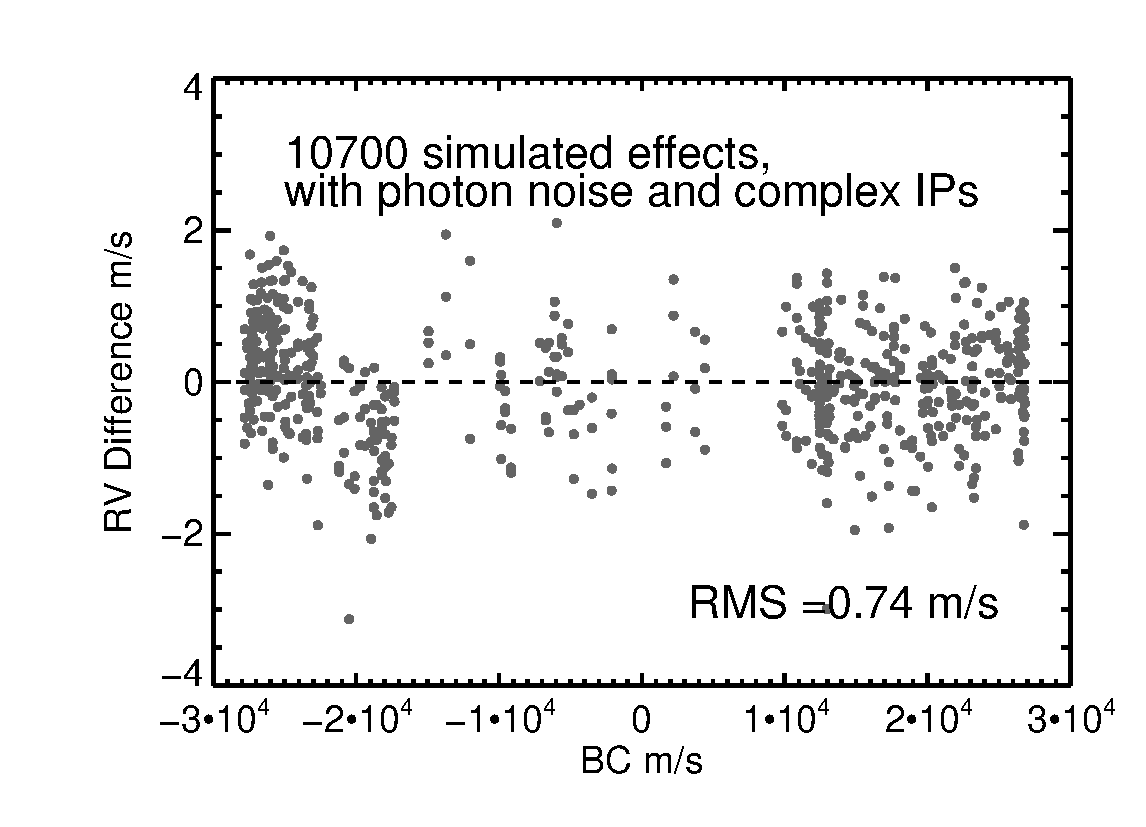
\includegraphics[scale=0.38]{telluric/10700-rv-bc-test0-test1.eps}}\
\caption{Effects of telluric lines manifested as correlation between
  RV and BC. Each point represents the difference in RV estimates for
  a pair of simulated spectra: one without telluric absorption, and
  one with telluric absorption on top of the stellar and iodine
  spectra. {\bf Top 2 panels:} To isolate the effects of telluric
  lines, the simulated spectra used for this plot do not have Poisson
  noise added, and they have simple one-component Gaussian IPs which
  have fixed width and thus the IP parameters are all fixed to the
  true values in the RV extraction. {\bf Middle 2 panels:} same as the
  top panels, but for simulated spectra with Poisson noise (same noise
  for the telluric and non-telluric spectrum pairs; and still the same
  simple IPs). {\bf Bottom 2 panels:} same as above, but for simulated
  spectra with Poisson noise and complex IPs that are similar to the
  ones in actual observations. IP parameters are not fixed in this
  case, so the code is fitting 12 additional parameters for the IP on
  top of the 3 for wavelength solution and Doppler shift (see
  Chapter~\ref{chap:doppler} for more details on the code).
\label{telluric:fig:sim}}
\end{figure}
%----------------------------------------------------------------


Micro-tellurics in the iodine region introduces RMS$=0.6$ m/s scatter
for GK stars (RV systematic error added in quadrature). Leaving
untreated, this would define the precision floor.

Additionally, it manifests as spurious signal at periods of a sidereal
year and harmonics, with an amplitude of 20 cm/s. This would affect
our ability to detect super-Earth in the habitable zone of GK stars
(Earth's signal is 8 cm/s). We have seen such spurious signal in Keck
data on many stars, and telluric contamination is one of the
contributing factors (see discussion for other factors).

For M stars... (probably worse)


%%%%%%%%%%%%%%%%%%%%%%%%%%%%%%%%%%%%%%%%%%%%%%%%%%%%%%%%%%%%%%%%%%%%%%%%%%%%
%%%%%%%%%%%%%%%%%%%%%%%%%%%%%%%%%%%%%%%%%%%%%%%%%%%%%%%%%%%%%%%%%%%%%%%%%%%%
\subsection{Remedies and Effectiveness}

There are several ways to remedy the adverse effects of telluric lines
on RV precision and accuracy: masking, modeling, or a combination of
both. HARPS works...

\subsubsection{Masking is an ineffective solution}

%----------------------------------------------------------------
% Table: RV RMS for various simulations
\renewcommand{\arraystretch}{1.2} % more row spacing for the table
\begin{deluxetable}{ccl}
\tabletypesize{\scriptsize}
\tablecaption{RV RMS for Simulations with Poisson Noise and Complex IP 
\label{telluric:tab:rmsmasking}}
\tablewidth{320pt}
\tablehead{
  \colhead{HD 185144} & \colhead{HD 10700} & \colhead{Simulation Conditions}
}
\startdata
1.26 m/s & 1.34 m/s & No tellurics \\
1.35 m/s & 1.42 m/s & With tellurics \\
1.35 m/s & 1.39 m/s & No tellurics, but masking telluric pixels \\
1.37 m/s & 1.43 m/s & With tellurics, and masking telluric pixels
\enddata
\end{deluxetable}
%----------------------------------------------------------------

% what do I mean when I talk about masking?
The simplest solution is to mask out telluric lines in the spectrum,
which means, in practice, locate the telluric-contaminated pixels and
flag them as bad pixels in the observed spectrum so that the
least-$\chi^2$ fitter will ignore them. For \keck\ or any
iodine-calibrated RV reduction, this also means masking out the
regions corresponding to locations of telluric lines in the
deconvolved stellar reference spectrum -- because the stellar
reference spectrum was taken at a different BC, the telluric lines
therein are shifted with respect to the ones in the epoch observation
as we try to match up the stellar lines in observed and reference
spectra. This ``double masking'' procedure is illustrated in
Figure~\ref{telluric:fig:dsstmask}. This is done ``dynamically'' in
the fitting process, in the sense that, for each iteration in the
least-$\chi^2$ minimization process, the contaminated pixels are
located according to the current wavelength solution parameters in
this fitting iteration. The wavelength solution changes from iteration
to iteration, and thus the masked pixels can change too.

%----------------------------------------------------------------
% Double masking of telluric lines
% plot made by converting pdf to eps. pdf comes from slides of CfASSP
% seminar talk, which can be found in ~/Ex.../Professional../..CfASSP../.
\begin{figure}
\subfloat{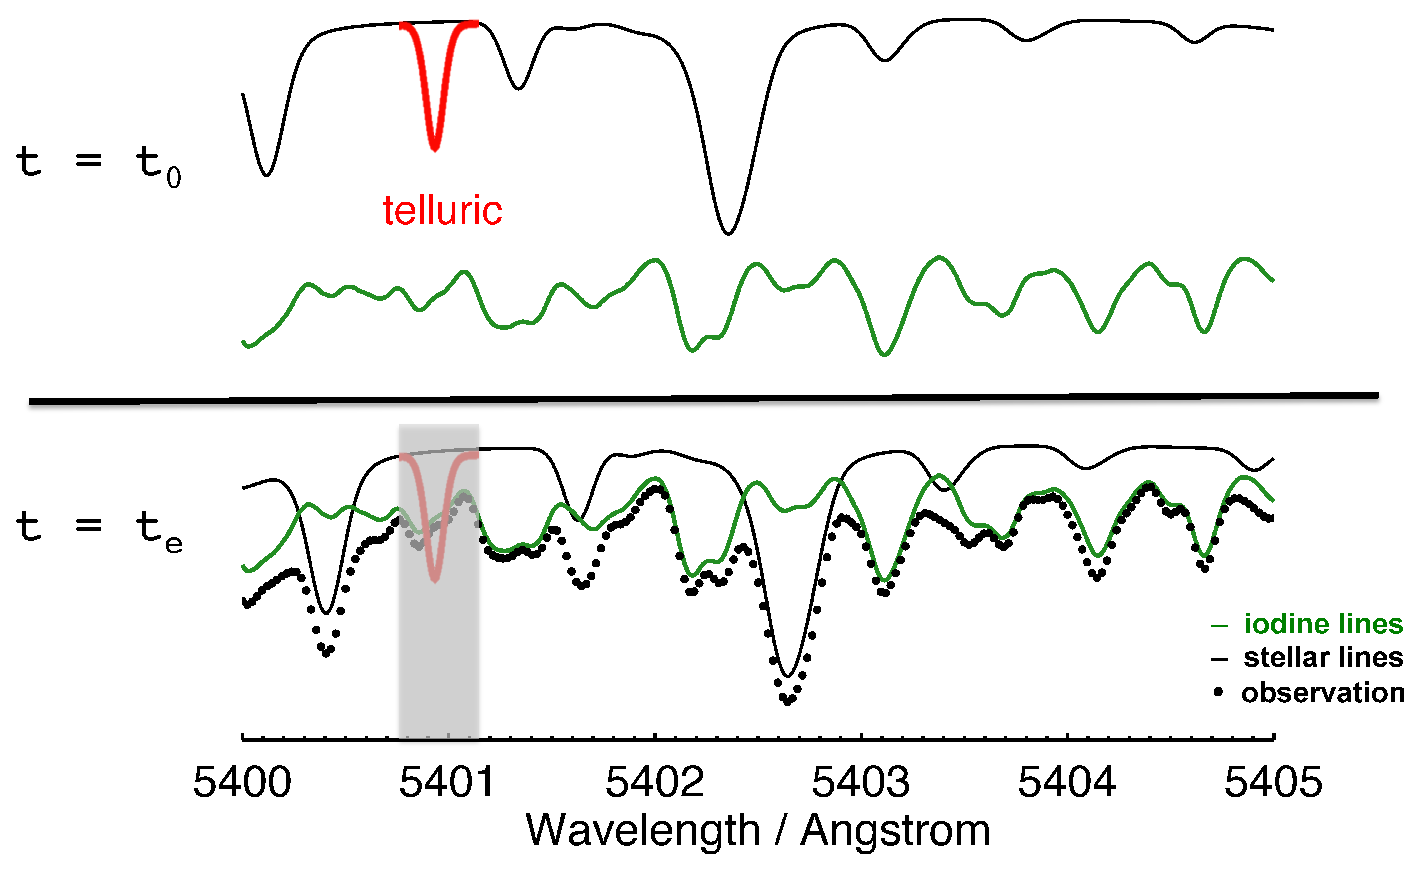
\includegraphics[scale=0.5]{telluric/dsst-mask1.eps}}\\
\subfloat{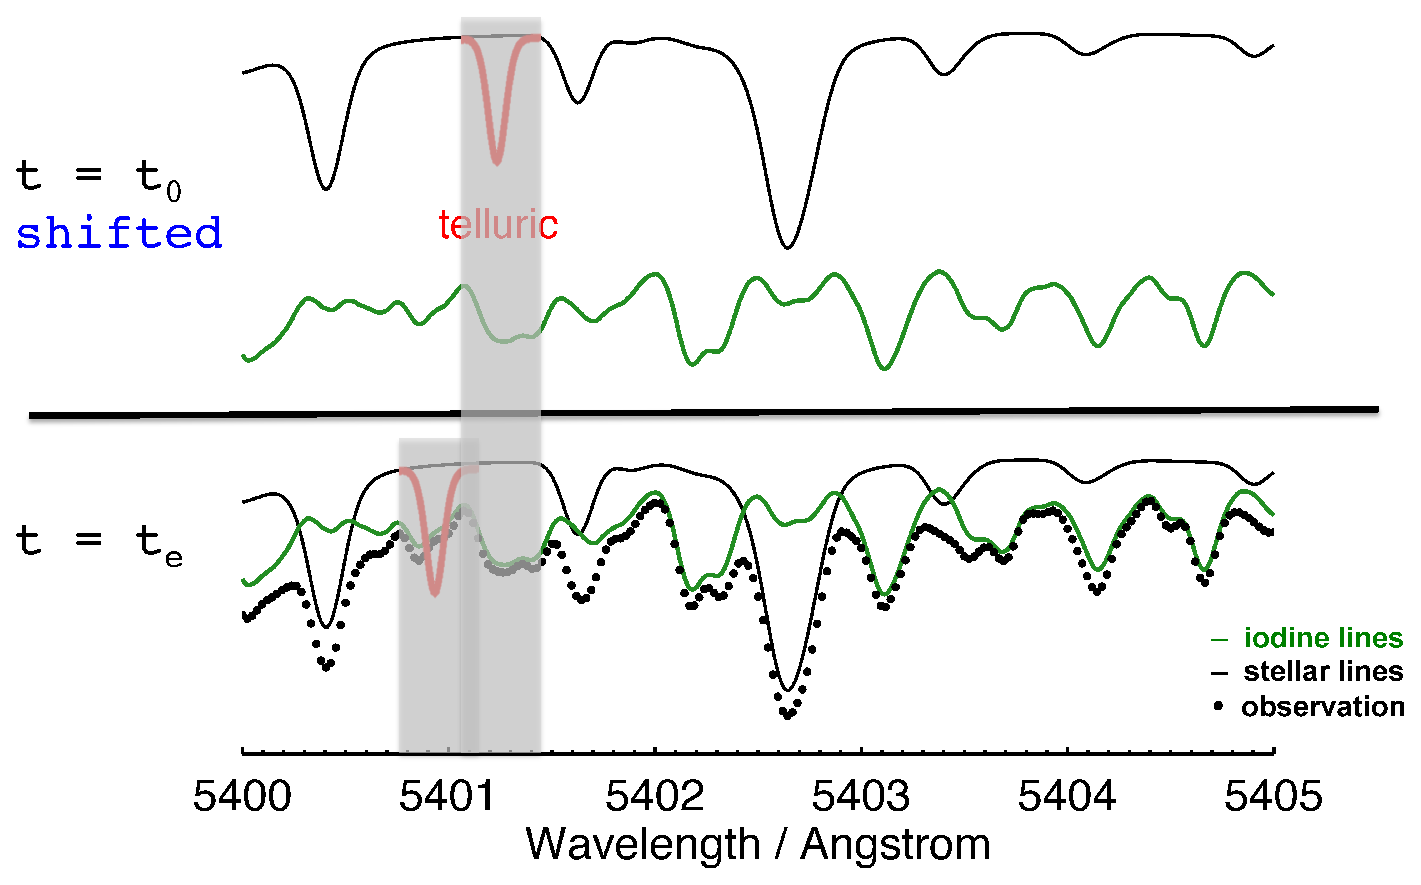
\includegraphics[scale=0.5]{telluric/dsst-mask2.eps}}
\caption{Illustration for how we mask telluric contaminated
pixels. The top panel shows how we mask the telluric lines (red solid
lines) in the epoch observation taken at $t=t_e$. The bottom panel
shows why we also need to mask pixels associated with telluric lines
in the deconvolved stellar reference spectrum taken at epoch $t=t_0$
and being shifted in order to model the observation.
\label{telluric:fig:dsstmask}}
\end{figure}
%----------------------------------------------------------------


% simulations and results
To investigate the effectiveness of masking, we performed RV
extraction on simulated spectra with or without telluric lines
injected and with or without masking (all with Poisson noise and
complex IP to mimic real observations as much as possible). For
stellar reference spectrum, we used the synthetic spectrum with
telluric lines. The results are tabulated in
Table~\ref{telluric:tab:rmsmasking}. In terms of improving RV
precision or reducing RV RMS, masking is very ineffective. The
additional errors it introduces diminish its merits. On the other
hand, masking does improve the accuracy to some degree: for example,
masking does remove the downward RV trend seen in HD 10700 data on the
bottom right plot of Figure~\ref{telluric:fig:sim} in the BC range
$[-3\times10^4,\ -2\times10^4]$ m/s. However, masking is an
ineffective way to mitigate the effects of telluric contamination
overall, especially since the RV errors and RV-BC trends are dominated
by photon noise and algorithmic errors (and other types of errors too
in real observations).

% why simple masking would not work for high precision/accuracy
So why masking does not work? First of all, it complicates the
$\chi^2$ surface and ``breaks'' the L-M fitter. Due to the ``dynamic''
nature of the mask mentioned above, the degrees of freedom for fitting
could change, because some telluric lines may shift in and out of this
spectral chunk as the wavelength solution changes. This would make the
fitter harder to converge or may create more loci for the fitter to
get stuck in, causing additional errors. Furthermore, masking is
throwing away iodine and stellar content embedded in these pixels
too. Finally, to ``mask'' the telluric lines out, one needs to pick a
flux threshold for the masks. This threshold must maintain a balance
between masking too much (throwing away too much iodine and stellar
information) and too little (leaving shallow telluric lines and line
wings untreated). In our study, we have chosen a flux threshold of
0.3\%, which means any pixel with telluric absorption deeper than
0.3\% will be masked (reference telluric spectrum is generated by
TERRASPEC at an altitude of 70$^{\degree}$, meaning deep oxygen lines,
and with precipitable water vapor (pwv) 0.8~mm, a little more than
typical \keck\ humidity). This masks 11\% of the spectral domain,
which is quite substantial and is very damaging to the RV precision,
but is almost the minimal amount of masking required to achieve some
RV accuracy improvement.

% how about masking in real observations?
We also applied telluric masking in RV reduction for real
observations, and saw no improvement over RV precision or
accuracy. This is because other effects dominate over telluric
absorption, as mentioned above, such as photon and algorithmic errors
and especially deconvolution errors in stellar reference spectrum,
which we will touch on in Section~\ref{keck:telluric:future} and
discuss in more detail in Section~\ref{keck:sec:dsst}.

% summarize
To summarize, masking sounds like a simple solution to the problem of
micro-telluric contamination, but it is actually complicated to
implement (for iodine-calibrated RV reduction) and it is ineffective
in terms of improving RV precision. We do not recommend masking as a
remedy for treating micro-telluric lines in iodine-calibrated RV
work. We believe the most effective way is to forward model telluric
lines, and combine that with some ``masking'' for deep or troublesome
telluric lines, which we discuss in the next subsection.

\subsubsection{How precisely does one need to model the tellurics?}


%----------------------------------------------------------------
% NEID Plot showing how much you need to model tellurics
\begin{figure}
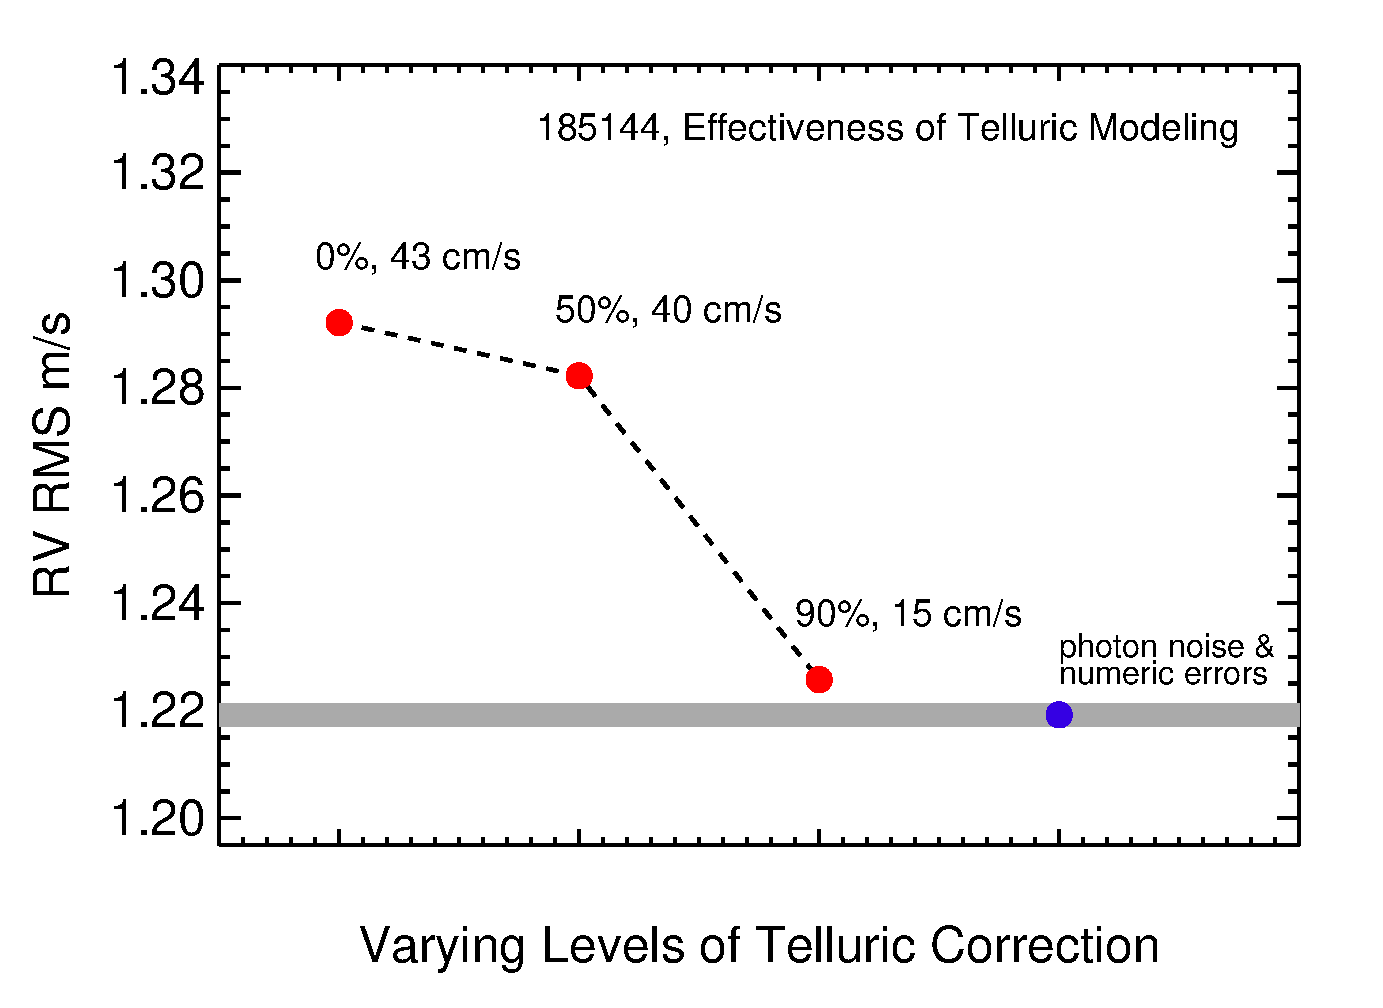
\includegraphics[scale=0.5]{telluric/neid.eps} 
\caption{Improvements in RV RMS for different ``level" of telluric
  modeling/removal. For example, the mid point labeled with ``50\%, 33 cm/s"
  means that if you model your telluric absorption lines to 50\% of
  their original depths, the effects of the residual telluric
  absorption will add 33 cm/s in quadrature to your final RV RMS. The
  blue point marks the RV RMS for simulations with Poisson noise and
  complex IP on HD 185144, which represents the photon-limited RV
  precision (subject to additional numeric or algorithmic errors; see
  Chapter~\ref{chap:conclusion} for more on the limitation of the
  Doppler code).
\label{telluric:fig:neid}}
\end{figure}
%----------------------------------------------------------------


% modeling is the way to go
The other way is to incorporate telluric lines as part of the iodine
RV forward modeling process, where water column density can either be
from a priori knowledge or an additional free parameter. In principle,
the oxygen column density can also be a free parameter, not because
the amount of oxygen varies on a noticeable level, but just to allow
some compensation for errors in atmospheric temperature and pressure
profile and so on. We do not fit for oxygen in our simulation or
treatment for real observations in this work for simplicity, and also
because the chunks contaminated with oxygen lines are in the reddest
part near 6300\AA, where the amount of iodine and stellar contents are
minimal anyway, and these chunks tend to be thrown away or heavily
de-weighted in the final RV weighting process.

% the goal of modeling
Modeling telluric absorption lines to high precision (below 1--2\% RMS
residual) can be a challenging task. There are several reasons for
this: lab measurements of a large number of water lines are
inaccurate, in terms of line depths, line positions, and line shapes;
and these line properties can also be uncertain due to change or a
lack of knowledge of the atmospheric conditions, such as wind, high
line-of-sight variations (e.g., water vapor), and mixing
uncertainties. For a summary of the state of the problem and paths
forward recommended by the RV community, see Section~4.6 in
\cite{eprv2015}. However, the goal here is not to model or ``remove''
the telluric lines perfectly, but to mitigate their impact on RV
precision and accuracy as much as possible. A central question is: how
well do we need to model telluric lines to reach a certain RV
precision \citep{eprv2015}?

% how well should we model?
To answer this question under the context of iodine-calibrated RV, we
performed RV extractions on the simulated HD 185144 data with telluric
absorption (all with pwv $=$ 1.0~mm, as described in
Section~\ref{keck:telluric:method}), incorporating forward modeling of
telluric lines with different levels of accuracy and using a stellar
reference spectrum free of tellurics. The results are illustrated in
Figure~\ref{telluric:fig:neid}. All three simulations were run with
simulated spectra of HD 185144 with pwv 1.0~mm, but the one labeled
``0\%'' has no telluric modeling in the RV extraction, while the one
labeled with ``50\%'' has synthetic telluric lines with pwv 0.5~mm in
the forward modeling process, and ``100\%'' meaning using telluric
model with pwv 1.0~mm, the same as the injected telluric lines. In
addition, we also used telluric model with pwv 1.1~mm in the forward
modeling, which basically produced the same RV RMS as the ``100\%''
simulation with no visible RV-BC trends or correlations. Extrapolating
between the results, a $\geq$90\% modeling accuracy for the water
lines would control the RV RMS contribution from tellurics to below
10~cm/s, which is near or beyond target precision for the next
generation RV spectrographs. This modeling is very easy to achieve in
reality.

% well actually vanking did a lot of heavy lifting
One important point to notice is that the reason why the damage of
10\% telluric modeling residual is controlled down to $\leq$10~cm/s is
the additional ``masking'' and weighting process in the Doppler code,
i.e., ``vanking'' (Chapter~\ref{chap:doppler}). In another word, a
combination of modeling (even only to 90\% precision) and statistical
weighting can effectively control the RV RMS introduced by tellurics
to $\leq$10~cm/s. Weighting plays a role in telluric contamination
remedy because it is essentially performing some ``masking'' on the
chunks that are badly contaminated by tellurics and/or have large
modeling residuals, such as the ones near 6300\AA\ with deep oxygen
lines and little stellar or iodine content.  Chunks with deep and
numerous oxygen lines are normally thrown out completely, and other
contaminated chunks which suffer from low precision will receive lower
weights and thus cast a lower impact on the final precision and
accuracy. In reality, we are using a combination of modeling and
masking or weighting to tackle problem of telluric contamination,
which we believe is the optimal solution for iodine-calibrated RVs.

\subsubsection{How about real observations?}

% what we did and what we saw
The situation is much more complicated for real observations, because
uncontrollable and unknown noise sources enter the picture. We have
tested both masking and preliminary modeling for real Keck RV
observations on HD 185144 and HD 10700. In the case of HD 185144, RV
RMS went down (from 2.57 m/s) after we applied masking (to 2.44 m/s)
or modeling (to 2.50 m/s), with visible changes in the RV-BC
trends. In the case of HD 10700, the RV RMS actually went up (from
3.05 m/s) after masking (to 3.26 m/s) or modeling (3.17 m/s), also
with visible changes in the RV-BC trend.

% well actually dsst dominates the errors anyway
If telluric contamination is dominating the spurious RV-BC trend, then
the results would be easier to interpret: other things, such as photon
noise and algorithmic errors mentioned above dominate the RV RMS, and
hence we see the almost arbitrary fluctuation of RV RMS with different
telluric remedies; and the changes we see in RV-BC trend are due to
the fact that we are removing the damages caused by telluric
contamination in RV accuracy. This is perhaps true for the cases of
masking, but is probably false for the cases with modeling, because
another important component is at play here: the deconvolved stellar
reference spectrum.

% DSST
For simulations, we have the privilege of using a true stellar
reference spectrum that is free of tellurics. For real observations,
when 



%%%%%%%%%%%%%%%%%%%%%%%%%%%%%%%%%%%%%%%%%%%%%%%%%%%%%%%%%%%%%%%%%%%%%%%%%%%%
%%%%%%%%%%%%%%%%%%%%%%%%%%%%%%%%%%%%%%%%%%%%%%%%%%%%%%%%%%%%%%%%%%%%%%%%%%%%
\subsection{Discussion and Future Work}\label{keck:telluric:future}


For redder bands, it is unclear at the moment what the requirement
would be, although some theoretical calculation by
\cite{2016AAS...22713719S} suggests that modeling to 1\% may not be
sufficient for reaching below 1~m/s in the near infrared.


We will try real observation, and see if a priori or floating water
column density parameter works better.

We hope to do a study on M dwarfs, because they are probably worse.

Important for MINERVA, HRS2, HPF2. Crucial for CARMENES, HPF, EPDS, SHREK,
ESPRESSO, SPiRou etc. White paper has suggested improvement on line
lists in HITRAN. EPRV2 has a lot of recommendations. That is the
future direction.





%%%%%%%%%%%%%%%%%%%%%%%%%%%%%%%%%%%%%%%%%%%%%%%%%%%%%%%%%%%%%%%%%%%%%%%%%%%%%%%%
\section{Erros Induced by Imperfect Stellar Reference Spectra}\label{keck:sec:dsst}

% Keck DSST section

For long, we believed that telluric contamination was the major culprit
behind the \keck\ RV-BC anomaly. However, the simulations in previous
section have revealed that tellurics probably only contribute a small
amount, mostly buried underneath photon noise and algorithmic
errors. We quickly focused our suspicion to DSST, because we saw the
differences in DSSTs before and after telluric cleaning (described in
Section~\ref{keck:telluric:real}), which are often larger than the
micro-telluric lines and could easily manifest as trends in the RV-BC
plane.

Any errors in the DSST, i.e., differences between the true stellar
spectrum and our assumed knowledge of truth (the DSST), are just like
persisting spectral contamination in the star's frame (instead of the
Earth's frame like the telluric contamination). Therefore, it beats
against the iodine lines as the stellar lines move back and forth
through the forest of iodine lines due to the Earth barycentric motion
and the star's intrinsic RV variation. As a result, it manifests as
anomalous RV-BC trends and adds bias and scatter to the final RVs.

We do know for sure that there are errors in the DSST, but the
question is how much, and more importantly, how much do these errors
translate into RV errors.


%----------------------------------------------------------------
% Effect of imperfect DSST
% plot made by ~/Exo.../Keck.../simulate.../msplot.pro, plot_name='3panel'
\begin{figure}
\subfloat[HD 185144]{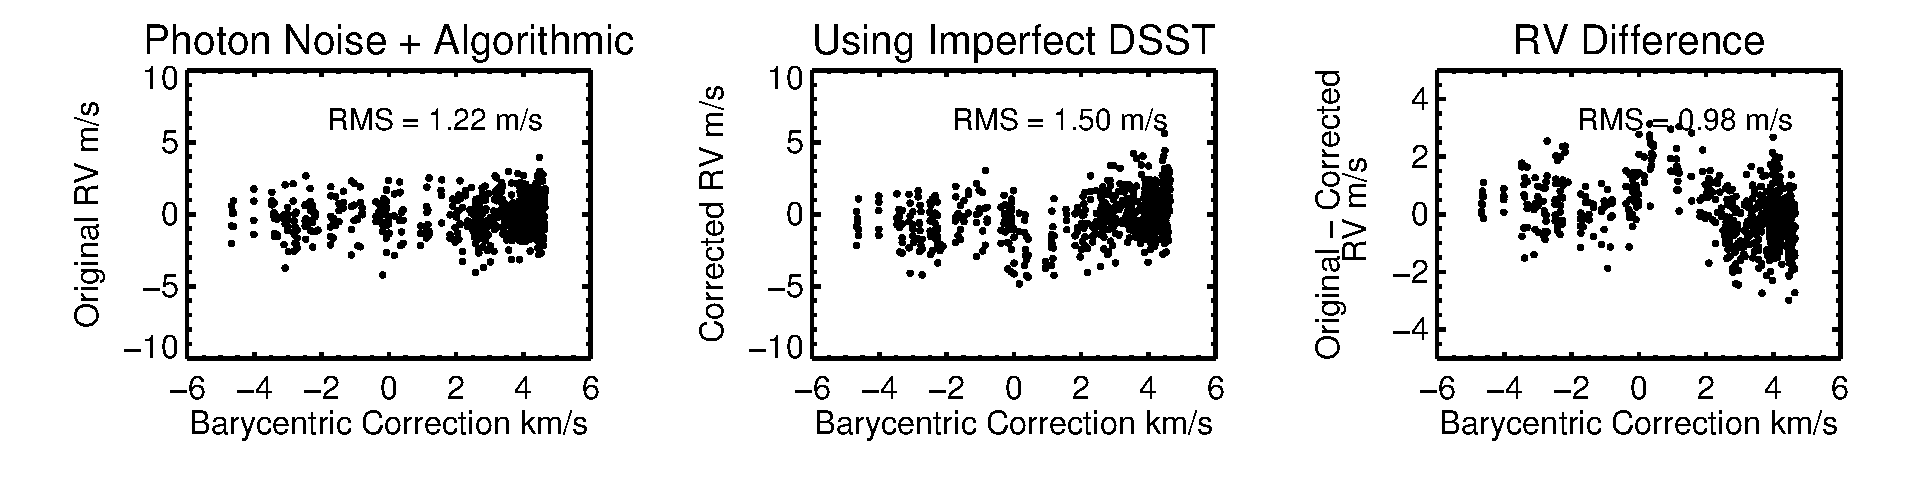
\includegraphics[scale=0.42]{keck/185144-rv-bc-3panel-test0-testd0.eps}}\
\subfloat[HD 10700]{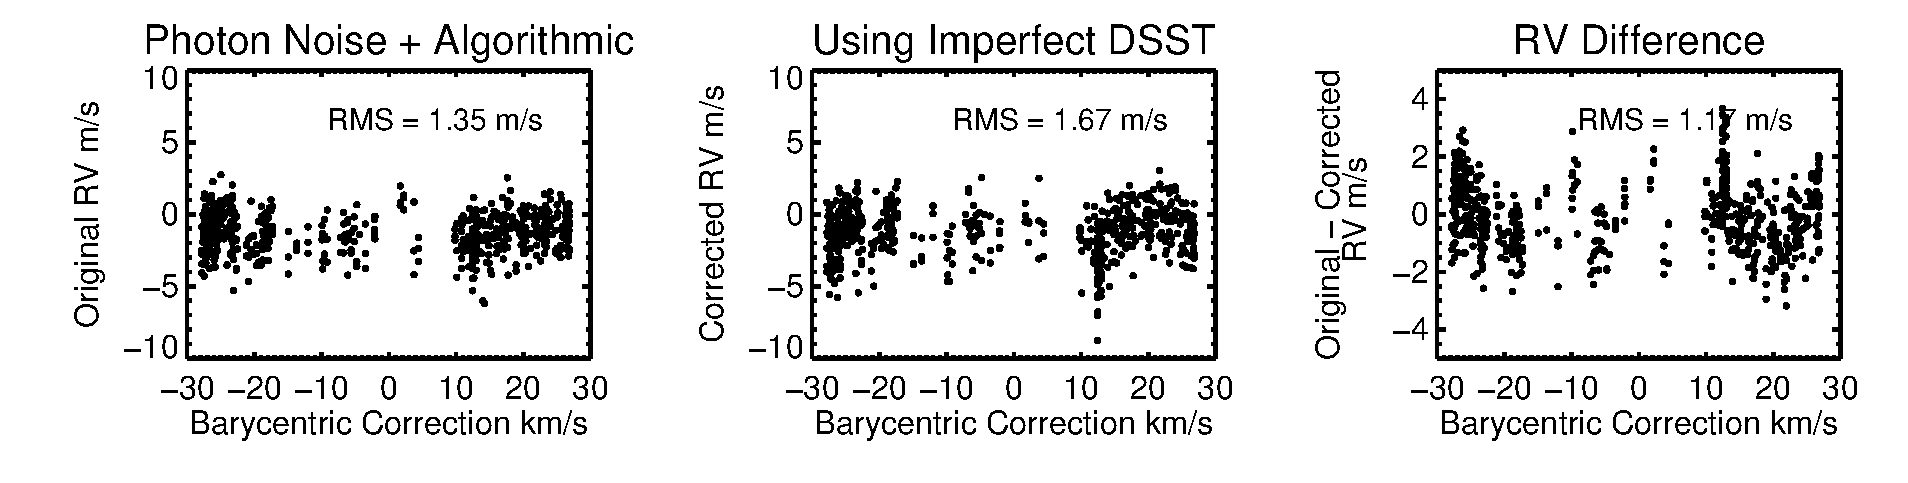
\includegraphics[scale=0.42]{keck/10700-rv-bc-3panel-test0-testd0.eps}}\
\caption{Effect of imperfect DSST on simulated data.
\label{keck:fig:dsst}}
\end{figure}
%----------------------------------------------------------------


%----------------------------------------------------------------
% Chunk illustration of effect of imperfect DSST
% plot made by ~/Exo.../Keck.../simulate.../msplot.pro, plot_name='makefakedsst','chunkcomp'
\begin{figure}
\subfloat{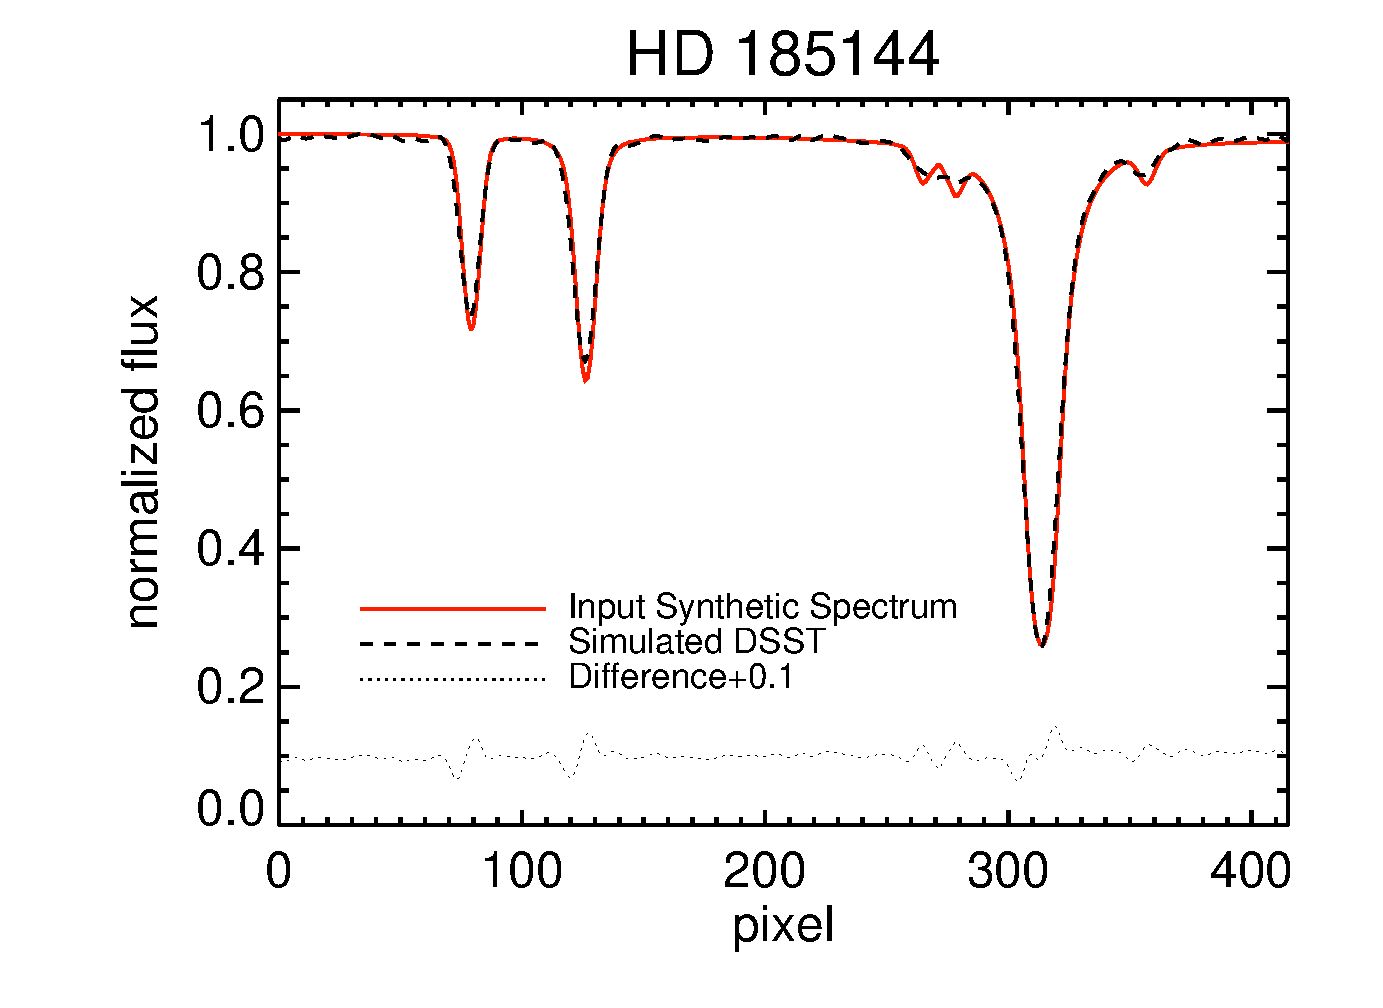
\includegraphics[scale=0.3]{keck/185144_makefakedsst_100.eps}}
\subfloat{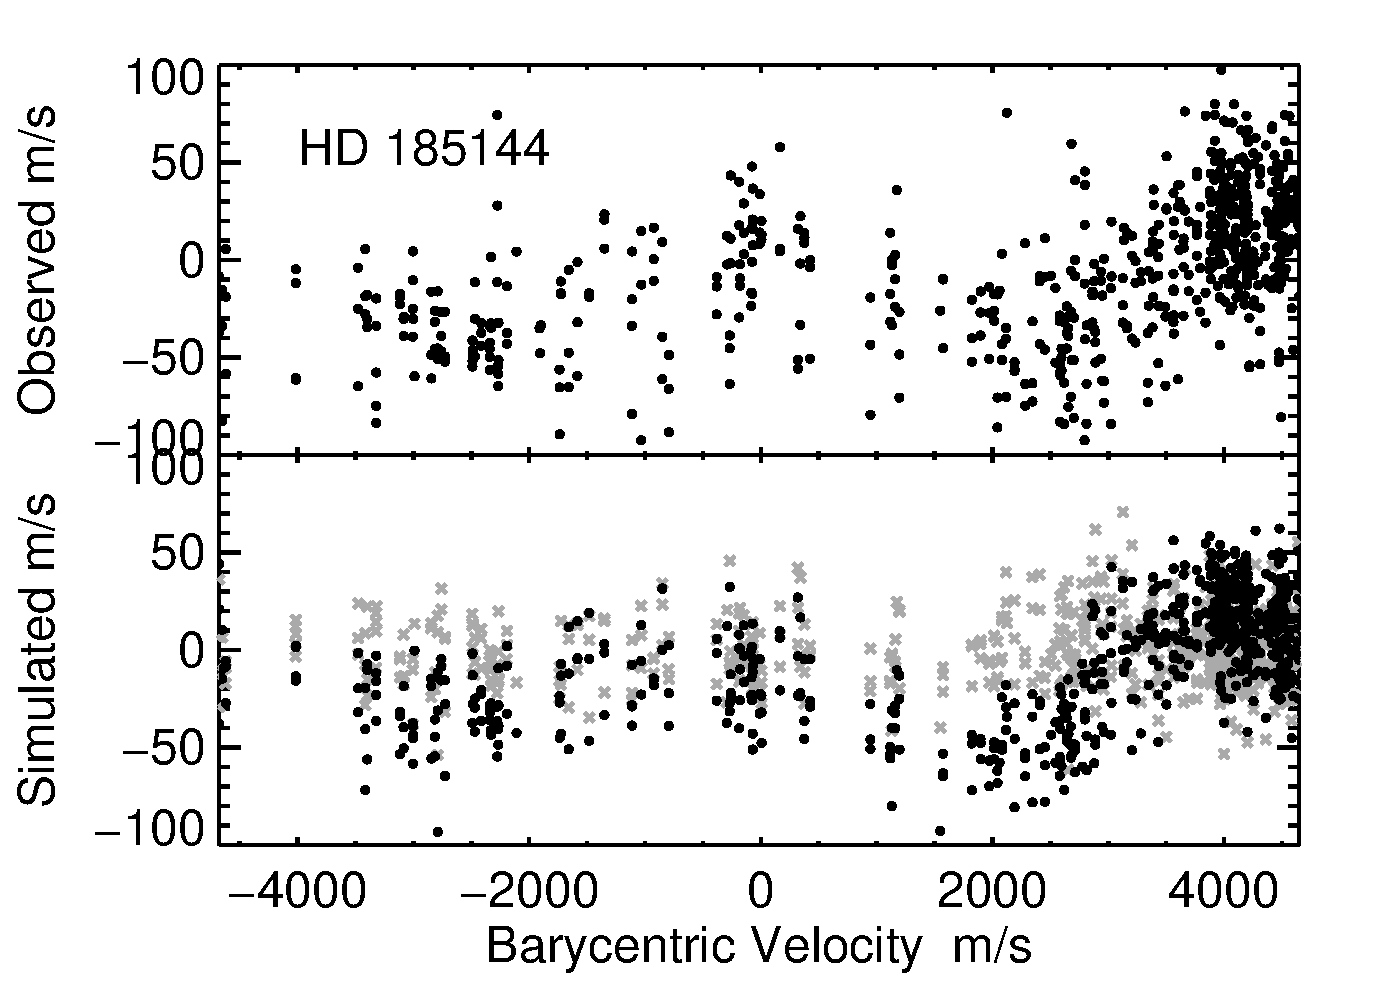
\includegraphics[scale=0.3]{keck/185144_chunkcomp_100.eps}}\
\subfloat{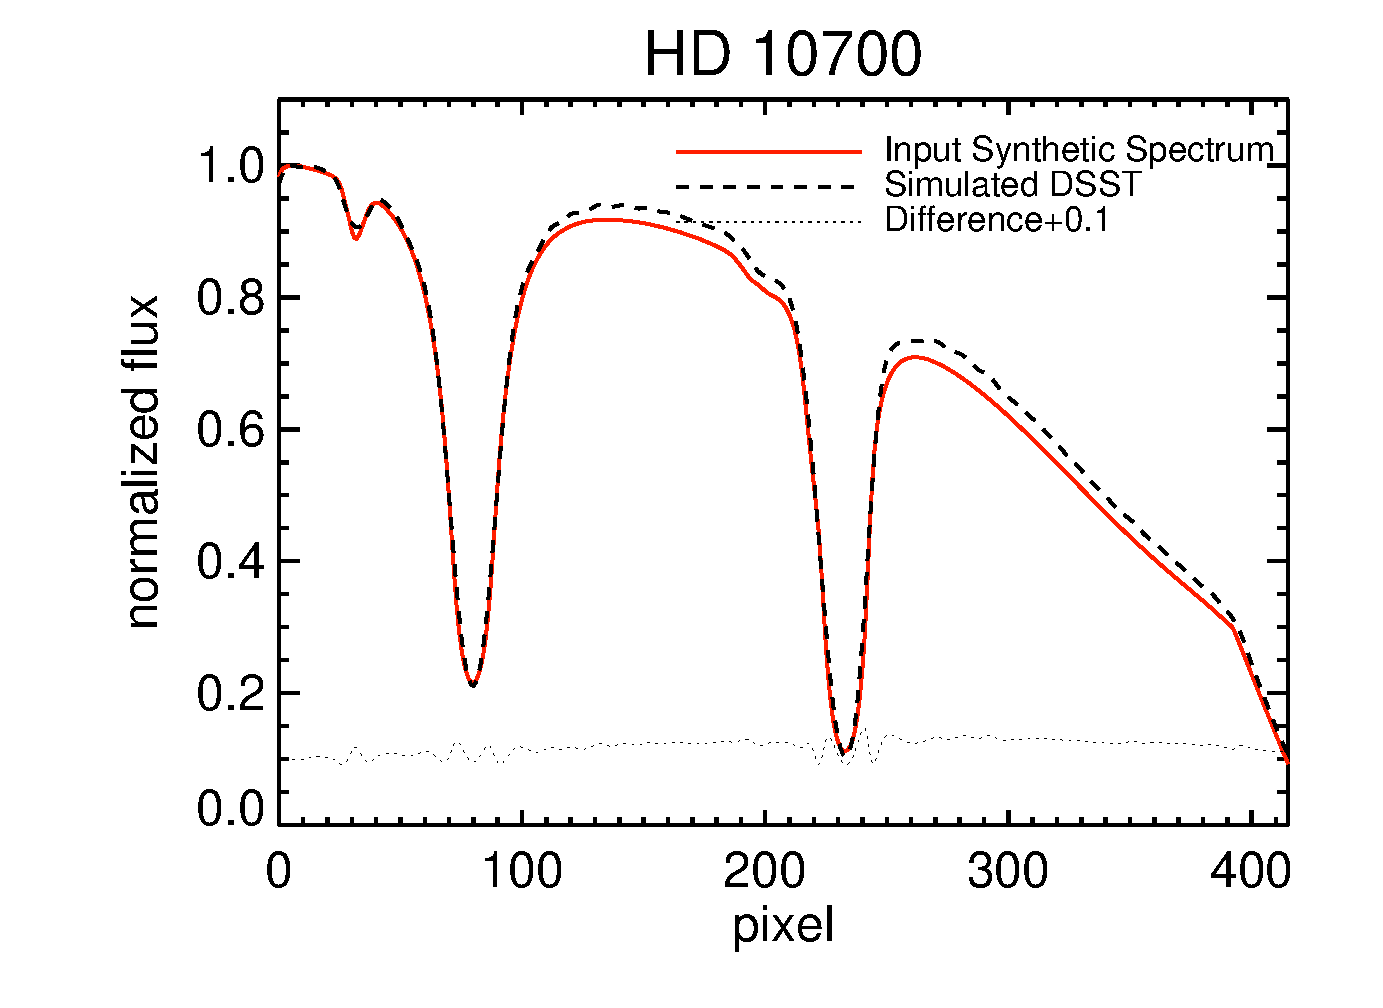
\includegraphics[scale=0.3]{keck/10700_makefakedsst_104.eps}}
\subfloat{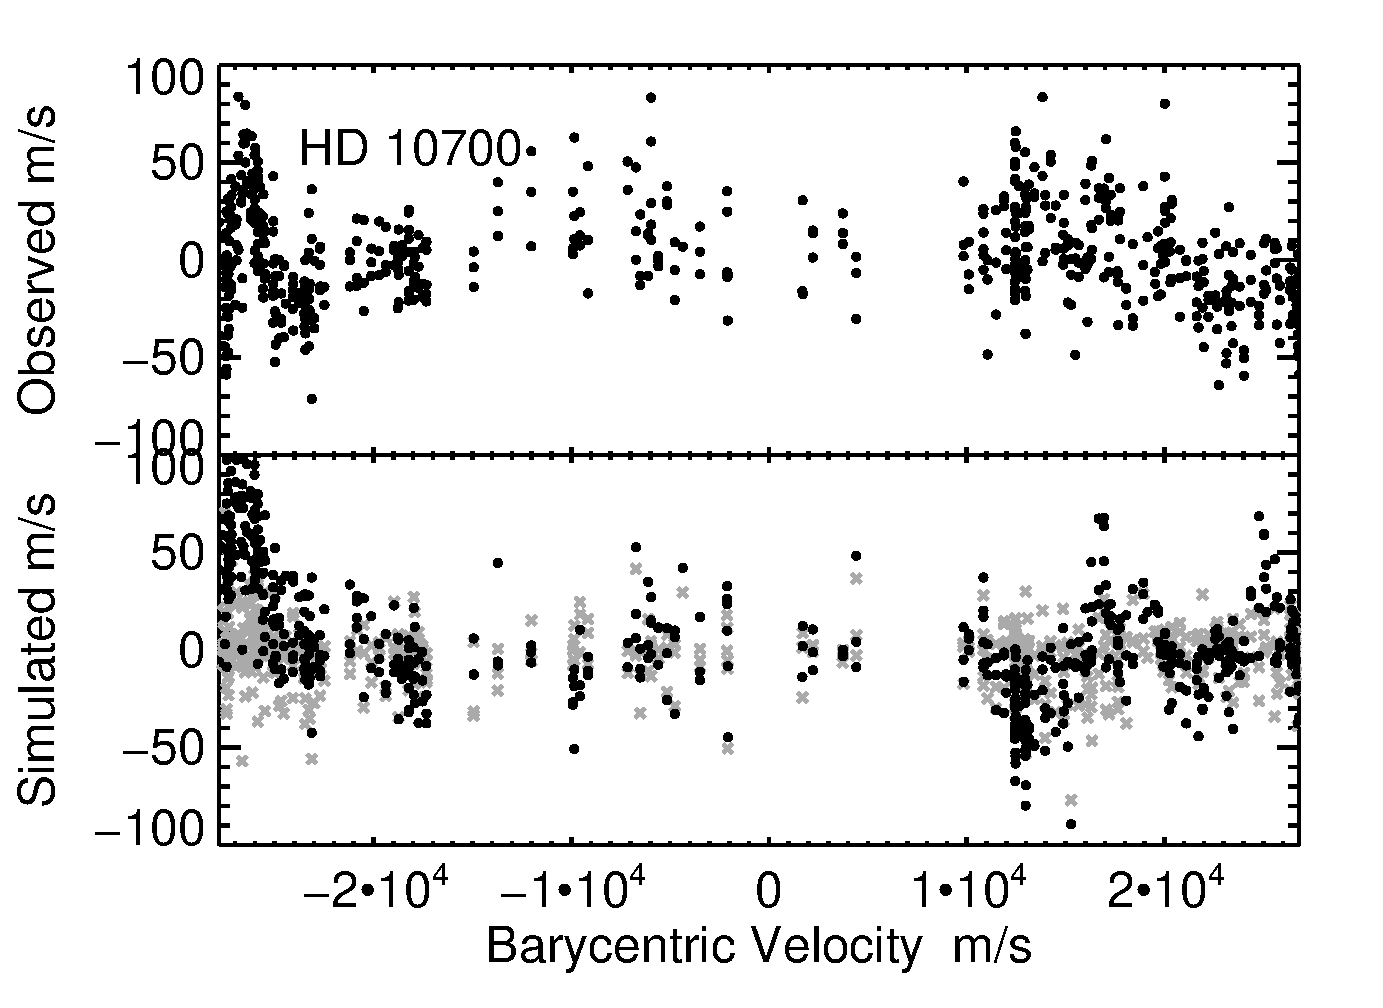
\includegraphics[scale=0.3]{keck/10700_chunkcomp_104.eps}}\
\caption{Effect of imperfect DSST on simulated data for a single
spectral chunk. HD 185144 is for a chunk near 5160\AA, and HD 10700 is
for a chunk around 5166\AA, which are spectral regions that tend to
receive high weights due to ample stellar lines and a lack of telluric
lines.
\label{keck:fig:dsstchunk}}
\end{figure}
%----------------------------------------------------------------




%%%%%%%%%%%%%%%%%%%%%%%%%%%%%%%%%%%%%%%%%%%%%%%%%%%%%%%%%%%%%%%%%%%%%%%%%%%%%%%%
\section{Numerical and Algorithmic Errors}\label{keck:sec:algorithm}

Solving the least-$\chi^2$ problem in a multi-dimensional, multi-modal
setting is not easy. Efficient as it might be in terms of
computational time, the least-$\chi^2$ algorithm employed by the CPS
Doppler code could give biased solution and comprise the RV precision
and accuracy. We performed simulations to probe the magnitude of such
errors.

Figure~\ref{keck:fig:algorithm} illustrates the RV scatter and RV-BC
trends induced by algorithmic errors -- the RVs plotted are from
simulations with no photon noise added, using the exact input spectrum
as the DSST, and the exact simple Gaussian IPs as the input. A perfect
algorithm should return all zeros for the RV, which is not the case
here. To probe the origin of this algorithmic errors a bit further, we
have run three sets of simulations at three different spectral
resolution (i.e., using different Gaussian IP widths). The amplitude
of the RV scatter decreases as the resolution increases, which is as
expected because shallower spectral lines probably translate to
shallower $\chi^2$ surfaces. However, the signature ``period'' or
length scale (in BC space) of the RV-BC trend does not change, which
is about 8~km/s or 6 pixels on the CCD. We are still investigating the
origin of this signature length scale (perhaps its in the blaze
normalization, or interpolation or rebinning algorithms, to name a
couple). The dichotomy in the red points (the fact that they split
into two RV groups) is probably due to the convergence criteria (which
are tuned for \keck\ resolution, and not sufficient for significantly
higher ones) and the algorithm's sensitivity in initial guesses. One
caveat is that because the IPs were fixed in the Doppler code run for
these simulations, the fitter only went through one pass (three free
parameters) instead of the standard two passes, where in the final
pass the wavelength dispersion scale is fixed. We will investigate
whether is this the major cause of algorithmic errors shown in
Figure~\ref{keck:fig:algorithm}. 


%----------------------------------------------------------------
% Plot showing algorithmic errors
% made by ~/Exo../Keck../simulate.../msplot.pro, in /msplot/.
\begin{figure}
\centering
\includegraphics[scale=0.65]{telluric/185144-rv-bc-rja01-rje01-rjf01.eps} 
\caption{RV vs.\ BC for HD 185144, for simulations with fixed simple
IPs and no photon noise added. The data plotted here are from
simulated spectral data with different IP widths (or spectral
resolution, $\sigma=1.7$ pixels corresponds to original \keck\
resolution). The origins of the RV scatters and trends in these plots
are purely algorithmic.
\label{keck:fig:algorithm}}
\end{figure}
%----------------------------------------------------------------

Figure~\ref{keck:fig:chunkalgorithm} shows an example chunk with
visible algorithmic errors. Again the top panel is showing real data,
and the bottom one is the simulated data (with photon noise and
complex IPs). This is a severe case, because its a chunk near 5900\AA\
which does not contain a large amount of stellar or iodine lines, and
therefore it is particularly challenging for the algorithm to find a
good $\chi^2$ minimum.

Unfortunately it is hard to quantify how much RV RMS the algorithmic
errors add to the RV budget, because the major damage comes from the
biases instead of the increased scatter (and the ``vanking'' procedure
breaks down because of this, unable to weigh the chunks effectively
and improve the precision). Figure~\ref{keck:fig:algorithm} suggests
that it can lead to spurious signals with considerable amplitude (1-3
m/s) for high SNR observations (the simulated observations here
essentially have infinitely SNR).


%----------------------------------------------------------------
% Chunk Plot showing algorithmic errors
% made by ~/Exo../Keck../simulate.../msplot.pro, in /msplot/.
\begin{figure}
\centering
\includegraphics[scale=0.5]{keck/chunkcomp-algorithm.eps} 
\caption{Real (top) or simulated (bottom) Keck RVs from a 2\AA\ chunk
from HD 185144 spectra showing RV systematic errors caused by
algorithmic errors. The RVs in the bottom panel are from the
simulations with complex IPs and photon noise.
\label{telluric:fig:chunkalgorithm}}
\end{figure}
%----------------------------------------------------------------


To list a few places in the Doppler code which may cause significant
numerical and algorithmic errors (not in any particular order): 
\begin{itemize}
\item The LM least-$\chi^2$ fitter: it can get stuck in local
  minima, and it may have reached the crude convergence criteria but not
  actually converged, and it is extremely sensitive to initial guesses.
\item The interpolation algorithm for interpolating or rebinning the model
  spectra. The current algorithm is not flux-conservative.
\item The simple linear fit to the blaze function in each chunk (each
  chunk contains 80 pixels).
\item ``Vanking'', or the final statistical weighting process, only
  takes into account RV scatter of each chunk but not biases.
\end{itemize}

Overall, it is not surprising at all that this decade-old Doppler code
fails to deliver precise RVs to the modern era standard. We discuss
the paths forward in Chapter~\ref{chap:conclusion}.



%%%%%%%%%%%%%%%%%%%%%%%%%%%%%%%%%%%%%%%%%%%%%%%%%%%%%%%%%%%%%%%%%%%%%%%%%%%%
%%%%%%%%%%%%%%%%%%%%%%%%%%%%%%%%%%%%%%%%%%%%%%%%%%%%%%%%%%%%%%%%%%%%%%%%%%%%
\section{Conclusion and Future Work}\label{keck:sec:conclusion}

In this chapter, we described our work on discovering and
characterizing three RV systematic error sources for \keck: telluric
contamination, errors in the DSST, and algorithmic errors. 

Telluric contamination, and in particular, micro-telluric lines, has a
small but non-negligible effects on the RV precision and accuracy. For
a typical G type star like the ones targeted by CPS, micro-tellurics
adds $\sim 0.6$~m/s to the RV error budget (in quadrature) and also a
spurious signal with an amplitude on the order of 10-20~cm/s if left
untreated. We have summarized the best strategies for treating
micro-telluric lines for precise RV using iodine calibrators in
Section~\ref{keck:sec:telluric}, which are masking deep lines,
cleaning DSST, forward modeling the telluric lines in RV extraction,
and assigning lower statistical weights to telluric-contaminated
chunks.

Errors in the DSSTs are one of current major RV systematic sources in
\keck\ RV data, and quite likely the largest one. It adds 1 m/s to the
RV error budget and creates a spurious signal with amplitude $\sim$ 1
m/s. RV-BC trends in simulated data match the ones seen in the
observed spectra among many spectral chunks, which pinned down this
source of error unambiguously. 

Algorithmic errors contribute a considerable amount to the current
\keck\ RV budget as well, and it is hard to imagine it would deliver
sub-m/s precision. After all, it is extremely challenging to find a
$\chi^2$ minimum on a complex surface with 15 dimensions (parameters)
using spectral data with 80 points (80 pixels per chunk) and
highly covariant model parameters. 

In terms of future work along these lines:

{\bf (1) Continuing the battle with telluric contamination: } We plan
to run simulations on an M star, HD 95735, also a RV standard. M stars
are particularly interesting because they may be more susceptible to
telluric contamination -- they have more stellar lines in the red
where the telluric lines are denser. We also plan to implement full
forward-modeling of telluric lines in real data reduction (as opposed
to our toy modeling with fixed water column density for all
dates/observations), and find out whether a priori or floating water
column density parameter works better. We plan to improve the DSST
cleaning process by incorporating forward modeling of telluric lines
in the ``piston Gaussians deconvolver'' that is currently used for
making DSST, instead of dividing them out. We hope to implement our
telluric correction package into the official CPS pipeline eventually,
which will be busily chewing \keck\ follow-up data on TESS targets
(many M dwarfs, undoubtedly) in the near future.

{\bf (2) Searching for a better DSST fabrication method: } We will
diagnose the origin of the DSST errors while searching for a better
deconvolution algorithm. It is possible that the current CPS
``deconvolution'' algorithm described in Section~\ref{keck:sec:dsst}
is sufficient, but the problem is in the normalization or some other
parts of the process. Nonetheless, it could be rewarding to jump out
of the current frame work and try another completely different
approach (e.g., constructing DSST from all the star$+$iodine frames,
which has been attempted by Andrew Vanderberg and John Johnson).

{\bf (3) Eliminating the numerical and algorithmic errors: } The CPS
Doppler code can certainly use an upgrade. However, in order to
eliminate a large portion of the algorithmic errors we are seeing now,
it probably means major structural changes to this lengthy and complex
legacy code written for early-1990 computers, regardless whether one
would like to stick with the L-M least-$\chi^2$ fitter. Therefore,
instead, I am building a new RV extraction code from scratch, using
Python and modern algorithms, which is one of the topics in
Chapter~\ref{chap:conclusion}.




\chapter{Characterization of Exoplanet Systems Using Radial
  Velocities}

% boottran and TERMS and Katherina's long-period planet paper.

%---------------------------------------------------------------------------
\section{BOOTTRAN: Uncertainties for Orbital Parameters Estimated
  Using Radial Velocities}\label{boottran:sec:boottran}

The uncertainties listed for the orbital parameter
estimates\footnote{Through out the paper and sometimes in this
  Appendix, we refer to the ``{\it estimates} of the parameters'' (as
  distinguished from the ``true parameters'', which are not known and
  can only be estimated) simply as the ``parameters''.} and transit
mid-time $T_c$ are calculated via bootstrapping
\citep{1981,davison1997bootstrap} using the package BOOTTRAN, which we
have made publicly available (see \S~\ref{sec:fit}). It is designed to
calculate error bars for transit ephemerides and the Keplerian
orbital fit parameters output by the RVLIN
package\citep{2009ApJS..182..205W}, but can also be a stand-alone
package. Thanks to the simple concept of bootstrapping, it is
computationally very time-efficient and easy to use.

The basic idea of bootstrap is to resample based on original data
to create bootstrap samples (multiple data replicates); then for
each bootstrap sample, derive orbital parameters or transit parameters
through orbital fitting and calculation. The ensemble of parameters
obtained in this way yields the approximate sampling distribution for
each estimated parameter. The standard deviation of this sampling
distribution is the standard error for the estimate.

We caution the readers here that there are regimes in which the
``approximate sampling distribution" (a frequentist's concept) is not
an estimate of the posterior probability distribution (a Bayesian
concept), and there are regimes (e.g., when limited sampling affects
the shape of the $\chi^2$ surface) where there are qualitative
differences and the bootstrap method dramatically underestimates
uncertainties \citep[e.g., long-period planets when the observations
  are not yet sufficient to pin down the orbital
  period;][]{Ford2005,Bender2012}. In situations with sufficient RV
data, good phase coverage, a sufficient time span of observations and
a good orbital fit, bootstrap often gives a useful estimate of the
parameter uncertainties. For the data considered in this paper, it
was not obvious that the bootstrap uncertainty estimate would be
accurate, as the time span of observations is only slightly longer than
the orbital period of planet $c$. Nevertheless, we find good agreement
between the uncertainty estimates derived from bootstrap and MCMC
calculations.

The radial velocity data are denoted as $\lbrace \vec{t},\ \vec{v},\ \vec{\sigma}
\rbrace$, where each $t_i$, $v_i$, $\sigma_i$ represents radial
velocity $v_i$ observed at time (BJD) $t_i$ with velocity uncertainty
$\sigma_i$. Extreme outliers should be rejected in order to preserve the
validity of our bootstrap algorithm. We first derive our estimates for
the true orbital parameters from the original RV data via orbital fitting,
using the RVLIN package \citep{2009ApJS..182..205W}: \beq \vec{\beta}
= \mu(\vec{t},\ \vec{v},\ \vec{\sigma}), \eeq where $\vec{\beta}$ is
the best fitted orbital parameters\footnote{As described in \S
  \ref{sec:fit}, this includes the $P$, $T_p$, $K$, $e$, and $\omega$
  for each planet, as well as $\gamma$, $\mbox{d}v/\mbox{d}t$ (if
  applicable), and velocity offsets between instruments/telescopes (if
  applicable) for the system.}. From $\vec{\beta}$, we derive $\lbrace
\vec{t},\ \vec{v}_{best}(\vec{\beta}) \rbrace$, the best-fit model
(here $\vec{t}$ are treated as predictors and thus fixed). Then we can
begin resampling to create bootstrap samples.

Our resampling plan is model-based resampling, where we draw from the
residuals against the best-fit model. For data that come from the
same instrument or telescope, in which case no instrumental offset
needs to be taken into account, we simply draw from all residuals,
$\lbrace \vec{v}-\vec{v}_{best} \rbrace$, with equal probability for
each $(v_i - v_{best,i})$. This new ensemble of residuals, denoted as
${\vec{r^*}}$, is then added to the best-fit model $\vec{v}_{best}$ to
create one bootstrap sample, $\vec{v^*}$ \footnote{We simply use the
  raw residual instead of any form of modified residual, because the
  RV data for any single instrument or telescope are usually close
  enough to homoscedasticity.}. Associated with ${\vec{r^*}}$, the
uncertainties $\vec{\sigma}$ are also re-assigned to $\vec{v^*}$ --
that is, if $v_j - v_{best,j}$ is drawn as $r_k$ and added to $v_k$ to
generate $v^*_k$, then the uncertainty for $v^*_k$ is set to be
$\sigma_j$.

For data that come from multiple instruments or multiple
telescopes, we incorporate our model-based resampling plan to include
stratified sampling. In this case, although data from each instrument
or telescope are close to homoscedastic, the entire set of data are
usually highly heteroscedastic due to stratification in
instrument/telescope radial velocity precision. Therefore, the
resampling process is done by breaking down the data into different
groups, $\lbrace \vec{v_1},\ \vec{v_2},\ \ldots \rbrace$, according to
instrument and/or telescope, and then resample within each
subgroup of data with the algorithm described in last paragraph. The bootstrap
sample is then $\vec{v^*} = \lbrace \vec{v^*}_1,\ \vec{v^*}_2,\ \ldots
\rbrace$.

To construct the approximate sampling distribution of the orbital
parameter estimates $\vec{\beta}$, we compute \beq \vec{\beta^*} =
\mu(\vec{t},\ \vec{v^*},\ \vec{\sigma^*}) \eeq for each bootstrap
sample, $\lbrace \vec{t},\ \vec{v^*},\ \vec{\sigma^*} \rbrace$. The
sampling distribution for each orbital parameter estimate $\beta_i$
can be constructed from the multiple sets of $\vec{\beta^*}$
calculated from multiple bootstrap samples
($\vec{\beta^*}^{(1)},\ \vec{\beta^*}^{(2)},\ \ldots$ from
$\vec{v^*}^{(1)},\ \vec{v^*}^{(2)},\ \ldots$). The standard errors for
$\vec{\beta}$ are simply the standard deviations of the sampling
distributions\footnote{The standard deviation of a sampling
  distribution is estimated in a robust way using the IDL function
  {\it robust\_sigma}, which is written by H. Fruedenreich based on
  the principles of robust estimation outlined in \cite{1983ured.book.....H}.}.

The sampling distribution of the estimated transit mid-time, $T_c$, is
calculated likewise. Here $T_c$ is the transit time for a certain
planet of interest in the system, and is usually specified to be the first
transit after a designated time $T$.  However, the situation is
complicated by the periodic nature of $T_c$. Our approach is to first
calculate, based on the original RV data, $T_{c0}$, the estimated
mid-time of the first transit after time $T_0$ (an arbitrary time
within the RV observation time window of $[\min(\vec{t}),\ \max(\vec{t})]$; $T_{c0}$ 
is also within this window).
Then
\beq
T_c = N\cdot P + T_{c0},
\eeq
where $P$ is the best-estimated period for this planet of interest,
and $N$ is the smallest integer that is larger than $(T - T_{c0})/P$.
Next we compute $T_{c0}^*$ for each bootstrap sample $\lbrace
\vec{t},\ \vec{v^*},\ \vec{\sigma^*} \rbrace$. Given that within the
time window of radial velocity observations
($[\min(\vec{t}),\ \max(\vec{t})]$), the phase of the planet should be
known well enough, it is fair to assume that $T_{c0}$ is an unbiased
estimator of the true transit mid-time. Therefore we assert that
$T_{c0}^*$ has to be well constrained and within the range of
$[T_{c0}-P^*/2,\ T_{c0}+P^*/2]$, where $P^*$ is the period estimated from
this bootstrap sample. If not, then we subtract or add multiple
$P^*$'s until $T_{c0}^*$ falls within the range. Then naturally
\beq
T_c^* = N\cdot P^* + T_{c0}^*.
\eeq
The ensemble of $T_c^*$'s gives the sampling distribution of $T_c$
and its standard error. Note that $T_c^*$ is not necessarily within
the rage of $[T_{c}-P/2,\ T_{c}+P/2]$.

Provided with the stellar mass $M_\star$ and its uncertainty, we
calculate, for each planet in the system, the standard errors for the
semi-major axis $a$ and the {\it minimum mass} of the planet $M_{\rm
  p,min}$ (denoted as $\msini$ in the main text as commonly seen in
literature, but this is a somewhat imprecise notation). As the first
step, the mass function is calculated for the best-fit $\vec{\beta}$
and each bootstrap sample $\vec{\beta^*}$,
\beq
f(P,K,e) = \frac{P K^3
  (1-e)^{3/2}}{2\pi G} = \frac{(M_p\cdot \sin i)^3}{(M_\star+M_p)^2}.
\eeq
The sampling distribution of $f(P,K,e)$ then gives the standard error
of the mass function. The minimum mass of the planet $M_{\rm p,min}$ 
is then calculated by assuming $\sin{i}=1$ and solving for $M_p$.
Standard error of $M_{\rm p,min}$ is derived through simple
propagation of error, as the covariance between $M_\star$ and
$f(P,K,e)$ is probably negligible.

For the semi-major axis $a$,
\beq
a^3 = \frac{P^2 G
  (M_\star+M_p)}{4\pi^2} \approx \frac{P^2 G (M_\star + M_{\rm p,min})}{4\pi^2}.
\eeq
The standard error of $P^2$ is calculated from its bootstrap sampling
distribution, and via simple propagation of error we obtain the
standard error of $a$ (neglecting covariance between $P^2$, $M_{\rm
  p,min}$, and $M_\star$).


%---------------------------------------------------------------------------
\section{Characterization of Planetary Systems Using BOOTTRAN}

Who cited our paper?

Mostly, TERMS. What is TERMS. What are the published systems with me
as coauthor doing this type of work.

What did I do for Ketherina's paper?

\chapter{The Discovery of HD 37605\lowercase{$c$} and a Dispositive
Null Detection of Transits of HD
37605\lowercase{$b$}}\label{chap:planets}

{\it
  The content in this chapter was published in ApJ, and the copyright
  belongs to IOP Publishing; all texts, figures, and tables are
  used in this thesis with permission. Most of the texts were written
  by Sharon Xuesong Wang, with the exception of
  Section~\ref{sec:intro} and Section~\ref{sec:activity} (both by
  Jason T.\ Wright), Section~\ref{SECN:DYNAMICS} (by Matthew
  J.\ Payne), and the first three paragraphs in Section~\ref{sec:most}
  (by Stephen R.\ Kane and Victoria Antoci).

  For figures and tables: Figure~\ref{mcmcplot} and \ref{dynamicplot}
  were made by Mathew J.\ Payne, Figure~\ref{photometry} and
  \ref{rotation} were made by Gregory W.\ Henry, and Figure~\ref{most}
  was made by Stephen R.\ Kane. The rest of the figures were made by
  Sharon Xuesong Wang. All tables were compiled by Sharon Xuesong
  Wang, although some of the data came from contributing authors:
  Table~\ref{smetable} was based on SME analysis results done by Jeff
  A.\ Valenti; Table~\ref{mcmctable} contains orbital parameters
  estimated using MCMC by Mathew J.\ Payne; the data in
  Table~\ref{phototable} are provided by Gregory W.\ Henry; and the
  data in Table~\ref{tab:most} are provided by Stephen R.\ Kane,
  Victoria Antoci, Diana Dragomir, and Jaymie M.\ Matthews.

}

\section{Introduction}\label{sec:intro}

%---------------------------------------------------------------------------
\subsection{Context}

Jupiter analogs orbiting other stars represent the first signposts of
true Solar System analogs, and the eccentricity distribution of these
planets with $a>3$ AU will reveal how rare or frequent true Jupiter
analogs are. To date, only 9 ``Jupiter analogs" have been
well-characterized in the peer reviewed literature\footnote{HD
  13931$b$ \citep{2010ApJ...721.1467H}, HD 72659$b$
  \citep{2011A&A...527A..63M}, 55 Cnc $d$ \citep{2002ApJ...581.1375M},
  HD 134987$c$ \citep{2010MNRAS.403.1703J}, HD 154345$b$ \citep[but
    with possibility of being an activity cycle-induced
    signal]{2008ApJ...683L..63W}, $\mu$ Ara $c$
  \citep{2007A&A...462..769P}, HD 183263$c$
  \citep{2009ApJ...693.1084W}, HD 187123$c$
  \citep{2009ApJ...693.1084W}, and GJ 832$b$
  \citep{2009ApJ...690..743B}.}  \citep[defined here as $P > 8$ years,
  $4 > M\sin{i} > 0.5\ \mjup$, and $e <
  0.3$;][exoplanets.org]{wrighteod}. As the duration of existing
planet searches approach 10--20 years, more and more Jupiter analogs
will emerge from their longest-observed targets
\citep{2012arXiv1205.2765W, 2012arXiv1205.5835B}.

Of the over 700 exoplanets discovered to date, nearly 200 are known to
transit their host star (\citealt{wrighteod}, exoplanets.org;
  \citealt{2011A&A...532A..79S}, exoplanet.eu), and many thousands more
candidates have been discovered by the {\it Kepler} telescope.  Of all
of these planets, only three orbit stars with $V<8$
\footnote{55 Cnc $e$ \citep{2004ApJ...614L..81M, 2011A&A...533A.114D},
%  HD 97658$b$ \citep{2011ApJ...730...10H, 2011arXiv1109.2549H}, %
%  turns out 97658b doesn't transit... ruled out by MOST.
  HD 189733 \citep{2005A&A...444L..15B}, and HD 209458
  \citep{2000ApJ...529L..41H, 2000ApJ...529L..45C}.}  and all have $P
< 4$ days.  Long period planets are less likely than close-in planets
to transit unless their orbits are highly eccentric and favorably
oriented, and indeed only 2 transiting planets with $P>20$ days have
been discovered around stars with $V<10$, and both have $e > 0.65$ (HD
  80606, \citealt{2009Natur.457..562L}, \citealt{2009MNRAS.396L..16F}; HD
  17156, \citealt{2007ApJ...669.1336F}, \citealt{2007A&A...476L..13B}; both
  highly eccentric systems were discovered first with radial
  velocities).

Long period planets not known to transit can have long transit windows
due to both the large duration of any edge-on transit and higher phase
uncertainties (since such uncertainties scale with the period of the
orbit). Long term radial velocity monitoring of stars, for instance
for the discovery of low amplitude signals, can produce collateral
benefits in the form of orbit refinement for a transit search and the
identification of Jupiter analogs
\citep[e.g.,][]{2009ApJ...693.1084W}. Herein, we describe an example
of both.

%---------------------------------------------------------------------------
\subsection{Initial Discovery and Followup}

The inner planet in the system, HD 37605$b$, was the first planet
discovered with the Hobby-Eberly Telescope (HET) at McDonald
Observatory \citep{cochran2004}.  It is a super Jupiter ($\msini =
2.41\ \mjup$) on an eccentric orbit $e=0.67$ with an orbital period in
the ``period valley'' \citep[$P=55$ days;][]{2009ApJ...693.1084W}.

W.C., M.E., and P.J.M.\, of the University of Texas at
Austin, continued observations in order to get a much better orbit determination
and to begin searching for transits. With the first new data in the
fall of 2004, it became obvious that another perturber was present in
the system, first from a trend in the radial velocity (RV) residuals
\citep[i.e., a none-zero $\mbox{d} v/\mbox{d} t$; ][]{wit2007}, and
later from curvature in the residuals. By 2009, the residuals to a
one-planet fit were giving reasonable constraints on the orbit of a
second planet, HD 37605$c$, and by early 2011 the orbital parameters
of the $c$ component were clear, and the Texas team was preparing the
system for publication.

%---------------------------------------------------------------------------
\subsection{TERMS Data}

The Transit Ephemeris Refinement and Monitoring Survey \citep[TERMS;][]{Kane2009} seeks
to refine the ephemerides of the known exoplanets orbiting bright,
nearby stars with sufficient precision to efficiently search for the
planetary transits of planets with periastron distances greater than a
few hundredths of an AU
\citep{2011EPJWC..1106005K, 2011ApJ...743..162P, 2011AJ....142..115D}.
This will provide the radii of planets not experiencing continuous high
levels of insolation around nearby, easily studied stars.

In 2010, S.M. and J.T.W.\ began radial velocity observations of HD
37605$b$ at HET from Penn State University for TERMS, to refine the
orbit of that planet for a future transit search. These observations,
combined with Keck radial velocities from the California Planet Survey (CPS)
consortium from 2006 onward, revealed that there was substantial
curvature to the radial velocity residuals to the original
\cite{cochran2004} solution. In October 2010 monitoring was
intensified at HET and at Keck Observatory by A.W.H., G.W.M., J.T.W.,
and H.I., and with these new RV data and the previously published
measurements from \cite{wit2007} they obtained a preliminary
solution for the outer planet. The discrepancy between the original
orbital fit and the new fit (assuming one planet) was presented at the
January 2011 meeting of the American Astronomical Society
\citep{terms2011aas}.

%---------------------------------------------------------------------------
\subsection{Synthesis and Outline}

In early 2011, the Texas and TERMS teams combined efforts and began
joint radial velocity analysis, dynamical modeling, spectroscopic
analysis, and photometric observations \citep{terms2012aas}. The
resulting complete two-planet orbital solution allows for a
sufficiently precise transit ephemeris for the $b$ component to be
calculated for a thorough transit search. We herein report the transit
exclusion of HD 37605$b$ and a stable dynamical solution to the
system.

In \S~\ref{sec:spec}, we describe our spectroscopic observations and
analysis, which provided the radial velocities and the stellar
properties of HD 37605. \S~\ref{sec:orbit} details the orbital
solution for the HD 37605 system, including a comparison with MCMC
Keplerian fits, and our dynamical analysis. We report our photometric
observations on HD 37605 and the dispositive null detection\footnote{A
  {\em dispositive} null detection is one that disposes of the
  question of whether an effect is present, as opposed to one that
  merely fails to detect a purported or hypothetical effect that may
  yet lie beneath the detection threshold.  The paragon of dispositive
  null detections is the Michelson-Morley demonstration that the
  luminiferous ether does not exist \citep{michelson1887}.} of
non-grazing transits of HD 37605$b$ in \S~\ref{sec:photo}. After
\S~\ref{sec:summary}, Summary and Conclusion, we present updates on
$\msini$ of two previously published systems (HD 114762 and HD 168443)
in \S~\ref{sec:correction}. In the Appendix we describe the algorithm
used in the package BOOTTRAN (for calculating orbital parameter error
bars; see \S~\ref{sec:fit}).



%%%%%%%%%%%%%%%%%%%%%%%%%%%%%%%%%%%%%%%%%%%%%%%%%%%%%%%%%%%%%%%%%%%%%%%%%%%%
\section{Spectroscopic Observations and Analysis}\label{sec:spec}
\subsection{HET and Keck Observations}
% HET obs, HRS intro (mode, wavelength range, RV precision)
Observations on HD 37605 at HET started December of 2003. In total,
101 RV observations took place over the course of almost eight years,
taking advantage of the queue scheduling capabilities of HET.
% queue schedule of HET
The queue scheduling of HET allows for small amounts of telescope time
to be optimally used throughout the year, and for new observing
priorities to be implemented immediately, rather than on next
allocated night or after TAC and scheduling process \citep{hetque2007}.
% HRS
The observations were taken through the High Resolution Spectrograph
\cite[HRS;][]{1998SPIE.3355..387T} situated at the basement of the HET
building. This
%temperature-controlled, % Jason striked this out. Not true any more?
fiber-fed spectrograph has a typical long-term Doppler error of 3 -- 5
\mps\ \citep{2009MNRAS.393..969B}. The observations were taken with the
spectrograph configured at a resolving power of $R=$60,000. For more
details, see \cite{cochran2004}.

% Keck obs, HIRES intro (mode, wavelength range, RV precision)
Observations at Keck were taken starting August 2006. A set of 33
observations spanning over five years were made through the HIRES
spectrometer \citep{1994SPIE.2198..362V} on the Keck I telescope,
which has a long-term Doppler error of 0.9 -- 1.5 \mps\
\citep[e.g.][]{2009ApJ...696...75H}. The observations were taken at a
resolving power of $R=$55,000. For more details, see
\cite{2009ApJ...696...75H} and \cite{2009ApJ...702..989V}.

% In general: RV obs, template obs
Both our HET and Keck spectroscopic observations were taken with an
iodine cell placed in the light path to provide wavelength standard
and information on the instrument response function\footnote{Some
  authors refer to this as the ``point spread function'' or the
  ``instrumental profile'' of the spectrograph.}  (IRF) for radial
velocity extraction \citep{1992PASP..104..270M, 1996PASP..108..500B}.
In addition, we also have observations taken without iodine cell to
produce stellar spectrum templates -- on HET and Keck,
respectively. The stellar spectrum templates, after being deconvolved
with the IRF, are necessary for both radial velocity extraction and
stellar property analysis. The typical working wavelength range for
this technique is roughly 5000 \AA -- 6000 \AA.


%----------------------------------------------------------------
\subsection{Data Reduction and Doppler Analysis}\label{sec:reduce}
In this section, we describe our data reduction and Doppler analysis
of the HET observations.  We reduced the Keck data with the standard
CPS pipeline, as described in, for example, \cite{2011ApJ...726...73H}
and \cite{2011ApJS..197...26J}.

% Data Reduction by REDUCE.
We have constructed a complete pipeline for analyzing HET data -- from
raw data reduction to radial velocity extraction. The raw reduction is
done using the REDUCE package by \cite{2002A&A...385.1095P}. This
package is designed to optimally extract echelle spectra from 2-D
images \citep{1986PASP...98..609H}. Our pipeline corrects for cosmic
rays and scattered light.
%It is robust in terms of cosmic ray removal and scattered light
%reduction. % changed by Jason into less 'robust' terms. lol
In order to make the data reduction process completely automatic, we
have developed our own algorithm for tracing the echelle orders of HRS
and replaced the original semi-automatic algorithm from the REDUCE
package.

% Stellar templates
After the raw data reduction, the stellar spectrum template is
deconvolved using IRF derived from an iodine flat on the night of
observation. There were two deconvolved stellar spectrum templates
(DSST) derived from HET/HRS observations and one from
Keck/HIRES. Throughout this work, we use the Keck DSST, which is of
better quality thanks to a better known IRF of HIRES and a
superior deconvolution algorithm in the CPS pipeline
\citep{2009ApJ...696...75H, 2011ApJ...726...73H}.

% Doppler code
Then the pipeline proceeds with barycentric correction and radial
velocity extraction for each observation. We have adopted the
Doppler code from CPS \citep[e.g.][]{
  2009ApJ...696...75H, 2011ApJ...726...73H, 2011ApJS..197...26J}. The
code is tailored to be fully functional with HET/HRS-formatted spectra,
and it is capable of working with either an HET DSST or a Keck one.

% Data reduction
% 104 HET observations: 2 DSST; 1 in 2012 not included in this paper;
% 2 low S/N, 1 twilight observation.
The 101 HET RV observations include 44 observations which
produced the published velocities in \cite{cochran2004} and
\cite{wit2007}, 34 observations also done by the Texas team in
follow-up work after 2007, and 23 observations taken as part of TERMS
program. We have performed re-reduction on these 44 observations
together with all the rest 57 HET observations through our
pipeline. This has the advantage of eliminating one free parameter in
the Keplerian fit -- the offset between two Doppler pipelines.

Two out of the 101 HET observations were excluded due to very low
average signal-to-noise ratio per pixel ($<20$), and one observation
taken at twilight was also rejected as such observation normally
results in low accuracy due to the significant contamination by the
residual solar spectrum (indeed this velocity has a residual of over
$100$ \mps\ against best Keplerian fit, much larger than the $\sim 8$
\mps\ RV error).

All the HET and Keck radial velocities used in this work (98 from HET
and 33 from Keck) are listed in Table \ref{rvtable}.


%----------------------------------------------------------------
\subsection{Stellar Analysis}\label{sec:sme}

% Results
HD 37605 is a K0 V star (V $\sim$ 8.7) with high proper motion at a
distance of 44.0 $\pm$ 2.1 pc \citep{esa1997,vanleeuwen2008}. We
derived its stellar properties based on analysis on a high-resolution
spectrum taken with Keck HIRES (without iodine cell in the light
path). Table \ref{smetable} lists the results of our
analysis\footnote{Note that the errors on the stellar radius $R_\star$
  and mass $M_\star$ listed in Table \ref{smetable} are not intrinsic to
  the SME code, but are 5\%$\times R_\star$ and 5\%$\times M_\star$. This is
  because the intrinsic errors reported by SME do not include the errors
  stemming from the adopted stellar models, and a more realistic
  precision for $R_\star$ and $M_\star$ would be around $\sim
  5$\%. Intrinsic errors reported by SME are $0.015\ L_\odot$ for
  $R_\star$ and $0.017\ \msol$ for $M_\star$.\label{foot:sme}}, including the
effective temperature $T_{\rm eff}$, surface gravity $\log{g}$, iron
abundance $[{\rm Fe/H}]$, projected rotational velocity $v\sin{i}$,
bolometric correction BC, bolometric magnitude $M_{\rm bol}$, stellar
luminosity $L_\star$, stellar radius $R_\star$, stellar mass $M_\star$
and age. HD 37605 is found to be a metal rich star ($[{\rm Fe/H}] \sim
0.34$) with $M_\star \sim 1.0\ \msol$ and $R_\star \sim 0.9
R_{\odot}$.

% The method, briefly
We followed the procedure described in \cite{valentifischer2005} and
also in \cite{2009ApJ...702..989V} with improvements. Briefly, the
observed spectrum is fitted with a synthetic spectrum using
Spectroscopy Made Easy \citep[SME; ][]{valentipiskunov1996} to derive
$T_{\rm eff}$, $\log{g}$, $[{\rm Fe/H}]$, $v\sin{i}$, and so on, which
are used to derive the bolometric correction BC and $L_\star$
consequently. Then an isochrone fit by interpolating tabulated
Yonsei-Yale isochrones \citep{2004ApJS..155..667D} using derived
stellar parameters from SME is performed to calculate $M_\star$ and
$\log{g_{\rm iso}}$ values (along with age and stellar radius). Next,
Valenti et al.~(2009) introduced an outside loop which re-runs SME
with $\log{g}$ fixed at $\log{g_{\rm iso}}$, followed by another
isochrone fit deriving a new log $\log{g_{\rm iso}}$ using the updated
SME results. The loop continues until $\log{g}$ values converge. This
additional iterative procedure to enforce self-consistency on log $g$
is shown to improve the accuracy of other derived stellar parameters
\citep{2009ApJ...702..989V}. The stellar radius and $\log{g}$ reported
here in Table \ref{smetable} are derived from the final isochrone fit,
which are consistent with the purely spectroscopic results. The
gravity ($\log{g} = 4.51$) is also consistent with the purely
spectroscopic gravity ($4.44$) based on strong Mg b damping wings, so
for HD 37605 the iteration process is optional.

% Yes these agree with other people's, do not panic.
\cite{cochran2004} reported the values of $T_{\rm eff}$, $\log{g}$,
and $[$Fe/H$]$ for HD 37605, and their estimates agree with ours
within 1$\sigma$ uncertainty. \cite{santos2005} also
estimated $T_{\rm eff}$, $\log{g}$, $[$Fe/H$]$, and $M_\star$, all of
which agree with our values within 1$\sigma$. Our stellar
mass and radius estimates are also consistent with the ones derived
from the empirical method by \cite{torres2010}.

% On vsini
Our SME analysis indicates that the rotation of the star ($v\sin{i}$)
is likely $< 1$ k\mps\ (corresponding to rotation period $\gtrsim 46$
days). We have used various methods to estimate stellar parameters
from the spectrum, including the incorporation of color and absolute
magnitude information and the Mg b triplet to constrain $\log{g}$, and
various macroturbulent velocity prescriptions.  All of these
approaches yield results consistent with an undetectable level of
rotational broadening, with an upper limit of 1-2 k\mps, consistent
with the tentative photometric period 57.67 days derived from the APT data (See
\S \ref{sec:apt}).



%%%%%%%%%%%%%%%%%%%%%%%%%%%%%%%%%%%%%%%%%%%%%%%%%%%%%%%%%%%%%%%%%%%%%%%%%%%%
\section{Orbital Solution}\label{sec:orbit}


\subsection{Transit Ephemeris}\label{sec:emph}

The traditional parameters for reporting the ephemerides of
spectroscopic binaries are $P, K, e, \omega$, and $T_p$, the last
being the time of periastron passage \citep{2009ApJS..182..205W}.
This information is sufficient to predict the phase of a planet at any
point in the future in principle, but the uncertainties in those
parameters alone are insufficient to compute the uncertainty in
orbital phase without detailed knowledge of the covariances among the
parameters.

This problem is particularly acute when determining transit or
secondary eclipse times for planets with near circular orbits, where
$\sigma_{T_p}$ and $\sigma_\omega$ can be highly covariant.  In such
cases the circular case is often not excluded by the data, and so the
estimation of $e$ includes the case $e=0$, where $\omega$ is
undefined.  If the best or most likely value of $e$ in this case is
small but not zero, then it is associated with some nominal value of
$\omega$, but $\sigma_\omega$ will be very large (approaching $\pi$).
Since $T_p$ represents the epoch at which the true anomaly equals
$0$, $T_p$ will have a similarly large uncertainty (approaching
$P$), despite the fact that the phase of the system may actually be
quite precisely known!

In practice even the ephemerides of planets with well measured
eccentricities suffer from lack of knowledge of the covariance in
parameters, in particular $T_p$ and $P$ (whose covariance is sensitive
to the approximate epoch chosen for $T_p$).  To make matters worse,
the nature of ``1$\sigma$'' uncertainties in the literature is
inconsistent.  Some authors may report uncertainties generated while
holding all or some other parameters constant (for instance, by seeing
at what excursion from the nominal value $\chi^2$ is reduced by 1),
while others using bootstrapping or MCMC techniques may report the
variance in a parameter over the full distribution of trials.  In any
case, covariances are rarely reported, and in some cases authors even
report the most likely values on a parameter-by-parameter basis rather
than a representative ``best fit'', resulting in a set of parameters
that is not self-consistent.

The TERMS strategy for refining ephemerides therefore begins with the
recalculation of transit time uncertainties directly from the archival
radial velocity data.  We used bootstrapping (see Appendix) with the
time of conjunction, $T_c$ (equivalent to transit center, in the
case of transiting planets) computed independently for each trial.
For systems whose transit time uncertainty makes definitive
observations implausible or impossible due to the accumulation of
errors in phase with time, we sought additional RV measurements to
``lock down'' the phase of the planet.


%----------------------------------------------------------------
\subsection{The 37605 System}\label{sec:fit}
% All velocities
There are in total 137 radial velocities used in the Keplerian fit for
the HD 37605 system. In addition to the 98 HET velocities and 33 Keck
ones (see \S \ref{sec:reduce}), we also included six\footnote{The
  velocity from observation on BJD $2,453,101.6647$ was rejected as it
  was from a twilight observation, which had both low precision
  ($\sigma_{\rm RV}=78.12$ \mps) and low accuracy (having a residual
  against the best Keplerian fit of over 100 \mps).} velocities from
\cite{cochran2004} which were derived from observations taken
with the McDonald Observatory 2.1 m Telescope (hereafter the 2.1 m
telescope).

% Package and code
We used the RVLIN package by \cite{2009ApJS..182..205W} to perform the
Keplerian fit. This package is based on the Levenberg\textendash
Marquardt algorithm and is made efficient in searching parameter space
by exploiting the linear parameters. The uncertainties of the
parameters are calculated through bootstrapping (with $1,000$
bootstrap replicates) using the BOOTTRAN package, which is described
in detail in the Appendix\footnote{The BOOTTRAN package is made
  publicly available online at http://exoplanets.org/code/ and the
  Astrophysics Source Code Library.}.

% Best fit parameters
The best-fit Keplerian parameters are listed in Table
\ref{fittable}. The joint Keplerian fit for HD 37605$b$ and HD 37605$c$
has 13 free parameters: the orbital period $P$, time of periastron
passage $T_p$, velocity semi-amplitude $K$, eccentricity $e$, and the
argument of periastron referenced to the line of nodes $\omega$ for
each planet; and for the system, the velocity offset between the
center of the mass and barycenter of solar system $\gamma$ and two
velocity offsets between the three telescopes ($\Delta_{\rm Keck}$ and
$\Delta_{\rm HET}$, with respect to the velocities from the 2.1 m
telescope as published in \citealt{cochran2004}). We did not include
any stellar jitter or radial velocity trend in the fit (i.e., fixed to
zero). The radial velocity signals and the best Keplerian fits for the
system, HD 37605$b$ only, and HD 37605$c$ only are plotted in the
three panels of Fig.~\ref{rvplot}, respectively.


% Below: bascially things I would like to draw reader's attention to.
% Planet masses and eccentricitie
Adopting a stellar mass of $M_\star=1.000 \pm 0.017\ \msol$ (as in Table
\ref{smetable}), we estimated the minimum mass ($\msini$) for HD
37605$b$ to be $2.802 \pm 0.011\ \mjup$ and $3.366 \pm 0.072\ \mjup$ for HD
37605$c$. While HD 37605$b$ is on a close-in orbit at $a=0.2831 \pm
0.0016$ AU that is highly eccentric ($e=0.6767 \pm 0.0019$), HD 37605$c$
is found to be on a nearly circular orbit ($e=0.013 \pm 0.015$) out at
$a=3.814 \pm 0.058$ AU, which qualifies it as one of the ``Jupiter
analogs''.

% Chi^2 map in P-Msini space
In order to see whether the period and mass of the outer planet, HD
37605$c$, are well constrained, we mapped out the $\chi_{\nu}^2$
values for the best Keplerian fit in the $P_c$-$M_c\sin{i}$ space
(subscript `$c$' denoting parameters for the outer planet, HD 37605$c$).
Each $\chi_{\nu}^2$ value on the $P_c$-$M_c\sin{i}$ grid was obtained
by searching for the best-fit model while fixing the period $P_c$ for the outer
planet and requiring constraints on $K_c$ and $e_c$ to maintain
$\msini$ fixed. As shown in Fig.~\ref{mmperplot}, our data are
sufficient to have both $P_c$ and $M_c\sin{i}$ well-constrained. This
is also consistent with the tight sampling distributions for $P_c$ and
$M_c\sin{i}$ found in our bootstrapping results.

% Telescope RMS v.s. errors, and jitter
The rms values against the best Keplerian fit are 7.86 \mps\ for HET,
2.08 \mps\ for Keck, and 12.85 \mps\ for the 2.1 m telescope. In the
case of HET and Keck, their rms values are slightly larger than their
typical reported RV errors ($\sim 5$ \mps\ and $\sim 1$ \mps,
respectively). This might be due to stellar jitter or underestimated
systematic errors in the velocities. We note that the $\chi_{\nu}^2$
is reduced to $1.0$ if we introduce a stellar jitter of 3.6 \mps\
(added in quadrature to all the RV errors).


%----------------------------------------------------------------
\subsection{Comparison with MCMC Results}\label{SECN:MCMC}


We compared our best Keplerian fit from RVLIN and uncertainties
derived from BOOTTRAN (abbreviated as RVLIN$+$BOOTTRAN
hereafter) with that from a Bayesian framework following
\cite{Ford2005} and \cite{Ford2006} (referred to as the MCMC analysis
hereafter). Table \ref{mcmctable} lists the major orbital parameters
from both methods for a direct comparison. Fig.~\ref{mcmcplot}
illustrates this comparison, but with the MCMC results presented in
terms of 2-D confidence contours for $P$, $e$, $K$, $\msini$, and
$\omega$ of both planets, as well as for $T_c$ of HD 37605$b$.

% By Matt P.
For the Bayesian analysis, we assumed priors that are uniform in log
of orbital period, eccentricity, argument of pericenter, mean anomaly
at epoch, and the velocity zero-point.  For the velocity amplitude
($K$) and jitter ($\sigma_j$), we adopted a prior of the form
$p(x)=(x+x_o)^{-1}[log(1+x/x_o)]^{-1}$, with $K_o=\sigma_{j,o}=1$ \mps,
i.e. high values are penalized. For a detailed discussion of priors,
strategies to deal with correlated parameters, the choice of the
proposal transition probability distribution function, and other
details of the algorithm, we refer the reader to the original papers:
\cite{Ford2005,Ford2006,2007ASPC..371..189F}. The likelihood for
radial velocity terms assumes that each radial velocity observation
($v_i$) is independent and normally distributed about the true radial
velocity with a variance of $\sigma_i^2+\sigma_j^2$, where $\sigma_i$
is the published measurement uncertainty.  $\sigma_j$ is a jitter
parameter that accounts for additional scatter due to stellar
variability, instrumental errors and/or inaccuracies in the model
(i.e., neglecting planet-planet interactions or additional, low
amplitude planet signals).

We used an MCMC method based upon Keplerian orbits to calculate a
sample from the posterior distribution \citep{Ford2006}. We calculated
5 Markov chains, each with $\sim 2 \times 10^8$ states. We
discarded the first half of the chains and calculate Gelman-Rubin test
statistics for each model parameter and several ancillary
variables. We found no indications of non-convergence amongst the
individual chains. We randomly drew $3\times 10^4$ solutions from the
second half of the Markov chains, creating a sample set of the
converged overall posterior distribution of solutions. We then
interrogated this sample on a parameter-by-parameter basis to find the
median and $68.27\%\,(1$$\sigma)$ values reported in Table
\ref{mcmctable}. We refer to this solution set below as the
``best-fit'' MCMC solutions.

We note that the periods of the two planets found in this system are
very widely separated ($P_c/P_b \sim 50$), so we do \emph{not} expect
planet-planet interactions to be strong, hence we have chosen to forgo
a numerically intensive N-body DEMCMC fitting procedure \citep[see
  e.g.][]{Johnson2011,2011ApJ...729...98P} as the non-Keplerian
perturbations should be tiny (detail on the magnitude of the
perturbations is provided in \S \ref{SECN:DYNAMICS}).  However, to
ensure that the Keplerian fits generated are stable, we took the
results of the Keplerian MCMC fits and injected those systems into the
Mercury n-body package \citep{Chambers1999} and integrated them
forward for $\sim 10^8$ years. This allows us to verify that all of the
selected best-fit systems from the Keplerian MCMC analysis are indeed
long-term stable. Further details on the dynamical analysis of the
system can be found in \S \ref{SECN:DYNAMICS}.

We assumed that all systems are coplanar and edge-on for the sake of
this analysis, hence all of the masses used in our n-body analyses are
\emph{minimum} masses. 

% revised by Matt
As shown in Table \ref{mcmctable} and Fig.~\ref{mcmcplot}, the
parameter estimates from RVLIN$+$BOOTTRAN and MCMC methods agree with
each other very well (all within 1-$\sigma$ error bar). In some cases,
the MCMC analysis reports error bars slightly larger than
bootstrapping method ($\sim$ 20\% at most). We note that the
relatively large MCMC confidence intervals are \emph{not}
significantly reduced if one conducts an analysis at a \emph{fixed}
jitter level (e.g. $\sigma_J = 3.5$\mps) unless one goes to an
extremely low jitter value (e.g. $\sim 1.5$\mps). That is, the larger
MCMC error bars do not simply result from treating the jitter as a
free parameter.
%
For the uncertainties on minimum planet mass $\msini$ and semi-major
axes $a$, the MCMC analysis does not incorporate the errors on the
stellar mass estimate.
%
Note here, as previously mentioned in \S~\ref{sec:emph}, that
the ``best-fit" parameters reported by the MCMC analysis here listed
in Table \ref{mcmctable} are not a consistent set, as the best
estimates were evaluated on a parameter-by-parameter basis, taking the
median from marginalized posterior distribution of each. Assuming no
jitter, The best Keplerian fit from RVLIN has a reduced chi-square
value $\chi_{\nu}^2 = 2.28$, while the MCMC parameters listed in Table
\ref{mcmctable} give a higher $\chi_{\nu}^2$ value of 2.91.

~~
%----------------------------------------------------------------
\subsection{Dynamical Analysis}\label{SECN:DYNAMICS}
%

% By Matt P., revised
We used the best-fit Keplerian MCMC parameters as the basis for a set
of long-term numerical (n-body) integrations of the HD 37605 system
using the Mercury integration package \citep{Chambers1999}. We used
these integrations to verify that the best-fit systems: (i) are
long-term stable; (ii) do not exhibit significant variations in their
orbital elements on the timescale of the observations (justifying the
assumption that the planet-planet interactions are negligible); (iii)
do not exhibit any other unusual features. We emphasize again that the
planets in this system are well separated and we do not expect any
instability to occur: for the masses and eccentricities in question, a
planet at $a_b \sim 0.28$ AU will have companion orbits which are
Hill stable for $a \gtrsim 0.83$ AU \citep{1993Icar..106..247G}, so while Hill
stability does not preclude outward scatter of the outer planet, the
fact that $a_c \sim 3.8 \gg 0.83$ AU suggests that the system will
be far from any such instability.

We integrated the systems for $> 10^8$ years ($\sim 10^7\times$ the
orbital period of the outer planet and $> 10^2\times$ the secular
period of the system), and plot in Fig. \ref{dynamicplot} the
evolution of the orbital elements $a,\ e$, \&\ $\omega$. On the
left-hand side of the plot we provide short-term detail, illustrating
that over the $\sim 10$ year time period of our observations, the
change in orbital elements will be very small.  On the right-hand side
we provide a much longer-term view, plotting $10^7$ out of $>10^8$ years
of system evolution, demonstrating that (i) the secular variation in
some of the elements (particularly the eccentricity of the outer
planet; see $e_c$ in red) over a time span of $\sim 4 \times 10^5$
years can be significant: in this case we see $0.03 < e_c < 0.11$, but
(ii) the system appears completely stable, as one would expect for
planets with a period ratio $P_c / P_b \sim 50$.  Finally, at the
bottom of the figure we display the range of parameter space covered
by the $e_i\cos{\omega_i},\ e_i\sin{\omega_i}$ parameters ($i=b$ in
blue for inner planet and $i=c$ in red for outer planet),
demonstrating that the orbital alignments circulate, i.e.\ they do not
show any signs of resonant confinement, which confirms our expectation
of minimal planet-planet interaction as mentioned before.
%(we weren't expecting to see anything, but it's good to
%check).

% added in revision by Matt
As noted above, our analysis assumed \emph{coplanar} planets. As such
the planetary masses used in these dynamical simulations are
\emph{minimum} masses. We note that for inclined systems, the larger
planetary masses will cause increased planet-planet perturbations. To
demonstrate this is still likely to be unimportant, we performed a
$10^8$ year simulation of a system in which $1 / \sin{i} = 10 $,
pushing the planetary masses to $\sim 30\ \mjup$. Even in such a
pathological system the eccentricity oscillations are only increased
by a factor of $\sim 2$ and the system remains completely stable for
the duration of the simulation.

% TTV
We also performed a separate Transit Timing Variation (TTV) analysis,
using the best-fit MCMC systems as the basis for a set of highly
detailed short-term integrations. From these we extracted the times of
transit and found a TTV signal $\sim 100$ s, or $\sim 0.001$ day,
which is much smaller than the error bar on $T_c$ ($\sim 0.07$
day). Therefore we did not take into account the effect of TTV when
performing our transit analysis in the next section.



%----------------------------------------------------------------
\subsection{Activity Cycles and Jupiter Analogs}\label{sec:activity}
% written by Jason

The coincidence of the Solar activity cycle period of 11 years and
Jupiter's orbital period near 12 years illustrates how activity cycles
could, if they induced apparent line shifts in disk-integrated stellar
spectra, confound attempts to detect Jupiter analogs around Sun-like
stars.  Indeed, \cite{1985srv..conf..311D} predicted apparent radial
velocity variations of up to 30 \mps\ in solar lines due to the Solar
cycle, and \cite{1987ApJ...316..771D} reported a tentative detection
of such a signal in NIR CO lines of 30 \mps\ in just 2 years, and noted
that such an effect would severely hamper searches for Jupiter
analogs.  That concern was further amplified when
\cite{1991LNP...390...19C} reported a positive correlation between
radial velocity and chromospheric activity in the active star
$\kappa^1$ Cet, with variations of order 50--100 \mps.

\cite{2008ApJ...683L..63W} found that the star HD 154345 has an
apparent Jupiter analog (HD 154345 $b$), but that this star also shows
activity variations in phase with the radial velocity variations.
They noted that many Sun-like stars, including the precise radial
velocity standard star HD 185144 ($\sigma$ Dra) show similar activity
variations and that rarely, if ever, are these signals well-correlated
with signals similar in strength to that seen in HD 154345 ($\sim$ 15
\mps), and concluded that the similarity was therefore likely just an
inevitable coincidence.  Put succinctly, activity cycles in Sun-like
stars are common \citep{1995ApJ...438..269B}, but few Jupiter analogs
have been discovered, meaning that the early concern that activity
cycles would mimic giant planets is not a severe problem.

Nonetheless, there is growing evidence that activity cycles can, in
some stars, induce radial velocity variations, and the example of HD
154345 still warrants care and concern.  Most significantly,
\cite{2011A&A...535A..55D} found a positive correlation between
chromospheric activity and precise radial velocity in the average
measurements of a sample of HARPS stars, and provided a formula for
predicting the correlation strength as a function of the metallicity
and effective temperature of the star.  Their formulae predict a value
of 2 \mps\ for the most suspicious case in the literature, HD 154345
(compared to an actual semiamplitude of $\sim$ 15 \mps), but are rather
uncertain.  It is possible that in a few, rare cases, the formula
might significantly underestimate the amplitude of the effect.

The top panel of Fig.~\ref{photometry} plots the T12 APT observations
from all five observing seasons (data provided in Table
\ref{phototable}; see details on APT photometry in
\S~\ref{sec:apt}). The dashed line marks the mean relative magnitude
($\Delta(b+y)/2$) of the first season.  The seasonal mean brightness
of the star increases gradually from year to year by a total of
$\sim 0.002$ mag, which may be due to a weak long-term magnetic cycle.
However, no evidence is found in support of such a cycle in the Mount
Wilson chromospheric Ca {\sc{ii}} H \& K indices \citep{svalue2010},
although the S values vary by approximately 0.1 over the span of a few
years. The formulae of \cite{2011A&A...528A.112L} predict a
corresponding RV variation of less than 2 \mps\ due to activity, far too
small to confound our planet detection with $K=49$ \mps.

Since we do not have activity measurements for this target over the
span of the outer planet's orbit in HD 37605, we cannot definitively
rule out activity cycles as the origin of the effect, but the strength
of the outer planetary signal and the lack of such signals in other
stars known to cycle strongly dispels concerns that the longer signal
is not planetary in origin.



%%%%%%%%%%%%%%%%%%%%%%%%%%%%%%%%%%%%%%%%%%%%%%%%%%%%%%%%%%%%%%%%%%%%%%%%%%%%
\section{The Dispositive Null Detection of Transits of HD 37605\lowercase{$b$}}\label{sec:photo}


% Overall
We have performed a transit search for the inner planet of the system,
HD 37605$b$. This planet has a transit probability of 1.595\% and a
predicted transit duration of 0.352 day, as derived from the stellar 
parameters listed in Table \ref{smetable} and the orbital parameters given 
in Table \ref{fittable}. From the minimum planet mass ($\msini = 2.802
\pm 0.011\ \mjup$; see Table \ref{fittable}) and the models of
\cite{planetradius2003}, we estimate its radius to be $R_{\rm p}= 1.1\ R_{\rm Jup}$. 
Combined with the stellar radius of HD 37605 listed in Table~\ref{smetable}, 
$R_\star=0.901 \pm 0.015\ R_{\odot}$, we estimate the transit depth to be 
1.877\% (for an edge-on transit, $i=90^{\circ}$). We used both ground-based 
(APT; \S \ref{sec:apt}) and space-based (MOST; \S \ref{sec:most}) 
facilities in our search. 


%----------------------------------------------------------------
\subsection{APT Observations and Analysis}\label{sec:apt}


% Photometric Observations with APT
The T12 0.8-m Automatic Photoelectric Telescope (APT), located at Fairborn 
Observatory in southern Arizona, acquired 696 photometric observations of
HD~37605 between 2008 January 16 and 2012 April 7. \cite{henry1999} provides 
detailed descriptions of observing and data reduction procedures with 
the APTs at Fairborn. The measurements reported here are differential 
magnitudes in $\Delta (b+y)/2$, the mean of the differential magnitudes 
acquired simultaneously in the Str\"omgren $b$ and $y$ bands with two
separate EMI 9124QB bi-alkali photomultiplier tubes.
% Photometric Precision
The differential magnitudes are computed from the mean of three 
comparison stars:
HD~39374 (V = 6.90, B$-$V = 0.996, K0 III), 
HD~38145 (V = 7.89, B$-$V = 0.326, F0 V), 
and HD~38779 (V = 7.08, B$-$V = 0.413, F4 IV).
This improves the precision of each individual measurement and helps to 
compensate for any real microvariability in the comp stars. Intercomparison 
of the differential magnitudes of these three comp stars demonstrates that all 
three are constant to 0.002 mag or better from night to night, consistent with
typical single-measurement precision of the APT 
\citep[0.0015-0.002 mag;][]{henry1999}.



% Commented 2012/09/29 - added new section 3.5 on stellar activity,
% moved there.
% Overall photometric fluctuation
%% The top panel of Fig.~\ref{photometry} plots the T12 APT observations
%% from all five observing seasons (data provided in Table
%% \ref{phototable}). The dashed line marks the mean relative magnitude
%% ($\Delta(b+y)/2$) of the first season.  The seasonal mean brightness
%% of the star increases gradually from year to year by a total of
%% $\sim~0.002$ mag, which may be due to a weak long-term magnetic cycle.
%% However, no evidence is found in support of such a cycle in the Mount
%% Wilson chromospheric Ca {\sc{ii}} H \& K indices \citep{svalue2010}.
%% This long-term photometric variability is too small to induce a RV
%% signal with $K \sim50$ \mps\ amplitude and so lends support to the
%% existence of HD~37605$c$.

% Describe how we prepare the data for transit analysis
% short paragraph replacing old paragraph 2
Fig.~\ref{photometry} illustrates the APT photometric data and our
transit search. As mentioned in \S~\ref{sec:activity}, the top panel
shows all of our APT photometry covering five observing seasons, which
exhibits a small increasing trend in the stellar brightness.
%
To search for the transit signal of HD 37605$b$, the photometric data
were normalized so that all five seasons had the same mean
(referred to as the ``normalized photometry" hereafter). The data were
then phased at the orbital period of HD~37605$b$, $55.01307$ days, and
the predicted time of mid-transit, $T_c$, defined as Phase~0.  The
normalized and phased data are plotted in the middle panel of
Fig.~\ref{photometry}.  The solid line is the predicted transit light
curve, with the predicted transit duration (0.352 day or 0.0064 phase
unit) and transit depth (1.877\% or $\sim 0.020$ mag) as estimated
above. The scatter of the phased data from their mean is $0.00197$
mag, consistent with APT's single-measurement precision, and thus
demonstrates that the combination of our photometric precision and the
stability of HD~37605 is easily sufficient to detect the transits of
HD~37605b in our phased data set covering five years.  A least-squares
sine fit of the phased data gives a very small semi-amplitude of
$0.00031~\pm~0.00011$ mag (consistent with zero) and so provides
strong evidence that the observed radial-velocity variations are not
produced by rotational modulation of surface activity on the star.


% Transit exclusion
The bottom panel of Fig.~\ref{photometry} plots the phased data around
the predicted time of mid-transit, $T_c$, at an expanded scale on the
abscissa.  The horizontal bar below the transit window represents the
$\pm$1$\sigma$ uncertainty on $T_c$ (0.138 day or 0.0025 phase unit for 
$T_c$'s near BJD $2,455,901.361$; see \S~\ref{sec:fit}).  The light curve 
appears to be highly clustered, or binned, due to the near integral orbital
period ($P \sim 55.01$ days) and consequent incomplete sampling from a 
single observing site.  Unfortunately, none of the data clusters chance 
to fall within the predicted transit window, so we are unable to rule out 
transits of HD~37605b with the APT observations.

% Overall period analysis, potential rotation period of the star
Periodogram analysis of the five individual observing seasons revealed no
significant periodicity between 1 and 100 days.  This suggests that the star 
is inactive and the observed $K \sim 200$ \mps\ RV signal (for HD~37605$b$) 
is unlikely to be the result of stellar activity.

Analysis of the complete, normalized data set, however, suggests a week 
periodicity of $57.67 \pm 0.30$ days with a peak-to-peak amplitude of just 
$0.0012 \pm 0.0002$ mag (see Fig.~\ref{rotation}).  We tentatively 
identify this as the stellar rotation period.  This period is consistent 
with the projected rotational velocity of $v\sin{i} < 1$ k\mps derived 
from our stellar analysis described in \S \ref{sec:sme}.  It is also 
consistent with the analysis of \cite{svalue2010}, who derived a Mount Wilson
chromospheric Ca {\sc{ii}} H \& K index of $S=0.165$, corresponding to
$\log R^\prime_{\rm HK} = -5.03$.  Together, these results imply a
rotation period $\gtrsim 46$ days and an age of $\sim 7$ Gyr (see 
Table~\ref{smetable}).  Similarly, \cite{age2002} find an age of $> 10$ Gyr 
using isochrones along with the Hipparcos parallax and space motion, 
supporting HD~37605's low activity and long rotation period.



%----------------------------------------------------------------
\subsection{MOST Observations and Analysis}\label{sec:most}


% MOST observations - paragraph from Vichi Antoci and Stephen K.
As noted earlier, the near-integer period of HD~37605$b$ makes it
difficult to observe from a single longitude. The brightness of the
target and the relatively long predicted transit duration creates
additional challenges for ground-based observations. We thus observed
HD~37605 during 2011 December 5--6 (around the predicted $T_c$ at BJD
$2,455,901.361$ as listed in Table \ref{fittable}) with the MOST
(Microvariability and Oscillations of Stars) satellite launched in
2003 \citep{2003PASP..115.1023W, 2004Natur.430...51M} in the Direct
Imaging mode. This observing technique is similar to ground-based CCD
photometry, allowing to apply traditional aperture and PSF procedures
for data extraction \citep[see e.g.][for
  details]{2006ApJ...646.1241R}. Outlying data points caused by, e.g.,
cosmic rays were removed.

% from Vichi, data reduction of MOST
MOST is orbiting with a period of $\sim$ 101 minutes (14.19
cycles per day, cd$^{-1}$), which leads to a periodic artifact induced by the
scattered light from the earthshine. This signal and its harmonics are
further modulated with a frequency of 1 cd$^{-1}$ originating from the
changing albedo of the earth. To correct for this phenomenon, we
constructed a cubic fit between the mean background and the stellar
flux, which was then subtracted from the data. The reduced and
calibrated MOST photometric data are listed in Table \ref{tab:most}.

% Transit exclusion
The MOST photometry is shown in Figure \ref{most} for the transit
window observations. The vertical dashed lines indicate the beginning
and end of the 1~$\sigma$ transit window defined by adding
$\sigma_{T_c}$ (0.069 day) on both sides of the predicted transit
duration of 0.352~days. The solid line shows the predicted transit
model for the previously described planetary parameters.
% significance for within the window with predicted depth
The rms scatter of the photometry is 0.17\%, and within the predicted
transit window there are 58 MOST observations. Therefore, the standard
error on the mean relative photometry (which is measured to be 0.00\%)
is 0.17\%$/\sqrt{58} = $ 0.022\%. This means that, for the predicted
transit window and a predicted depth of 1.877\%, we can conclude a
null detection of HD 37605$b$'s transit with extremely high confidence
(149$\sigma$).

% Grazing constraint and chance of missing the transit window
% grazing transit - need Stephen's numbers here
Note that the above significance is for an edge-on transit with an
impact parameter of $b = 0.0$. A planetary trajectory across the
stellar disk with a higher impact parameter will produce a shorter
transit duration. However, the gap between each cluster of MOST
measurements is 0.06~days which is 17\% of the edge-on transit
duration. In order for the duration to be fit within the data gaps,
the impact parameter would need to be $b > 0.996$. To estimate a more
conservative lower limit for $b$, we now assume the most unfortunate
case where the transit center falls exactly in the middle of one of
the measurement gaps, and also consider the effect of limb darkening
by using the non-linear limb darkening model by
\cite{2002ApJ...580L.171M} with their fitted coefficients for HD
209458. Even under this scenario, we can still conclude the null
detection for any transit with $b<0.951$ at $\gtrsim 5\sigma$ (taking
into account that there are at least $\sim$ 20 observations will fall
within the transit window in this case, though only catching the
shallower parts of the transit light curve).
% very dense planet

All of the above is based on the assumption that the planet has the
predicted radius of 1.1 $R_{\rm Jup}$. If in reality the planet is so
small that even a $b=0$ transit would fall below our detection
threshold, it would mean that the planet has a radius of $< 0.36\ R_{\rm
  Jup}$ (a density of $>$ 74.50 g$/$cm$^3$), which seems unlikely.
% chance of missing the window from Tc errors?
It is also very unlikely that our MOST photometry has missed the
transit window completely due to an ill-predicted $T_c$. In the
sampling distribution of $T_c$ from BOOTTRAN (with 1000 replicates;
see \S~\ref{sec:fit} and Appendix), there is no $T_c$ that would put
the transit window completely off the MOST coverage. In the
marginalized posterior distribution of $T_c$ calculated via MCMC (see
\S~\ref{SECN:MCMC} and Fig.~\ref{mcmcplot}), there is only 1 such
$T_c$ out of $3 \times 10^4$ (0.003\%).



%%%%%%%%%%%%%%%%%%%%%%%%%%%%%%%%%%%%%%%%%%%%%%%%%%%%%%%%%%%%%%%%%%%%%%%%%%%%
\section{Summary and Conclusion}\label{sec:summary}

% Summary of the paper
In this paper, we report the discovery of HD 37605$c$ and the
dispositive null detection of non-grazing transits of HD 37605$b$, the first
planet discovered by HET. HD 37605$c$ is the outer planet of the
system with a period of $\sim 7.5$ years on a nearly circular orbit
($e=0.013$) at $a=3.814$ AU. It is a ``Jupiter analog'' with $\msini =
3.366\ \mjup$, which adds one more sample to the currently still small
inventory of such planets (only 10 including HD 37605$c$; see \S
\ref{sec:intro}). The discovery and characterization of ``Jupiter
analogs'' will help understanding the formation of gas giants as well
as the frequency of true solar system analogs. This discovery is a
testimony to the power of continued observation of planet-bearing
stars.

Using our RV data with nearly 8-year long baseline, we refined the
orbital parameters and transit ephemerides of HD 37605$b$. The
uncertainty on the predicted mid-transit time was constrained down to
0.069 day (at and near $T_c = 2,455,901.361$ in BJD), which is small
compared to the transit duration (0.352 day). In fact, just the
inclusion of the two most recent points in our RV data have reduced
the uncertainty on $T_c$ by over 10\%. We have performed transit
search with APT and the MOST satellite. Because of the near-integer
period of HD~37605$b$ and the longitude of Fairborn Observatory, the
APT photometry was unable to cover the transit window. However, its
excellent photometric precision over five observing seasons enabled us
to rule out the possibility of the RV signal being induced by stellar
activity. The MOST photometric data, on the other hand, were able to
rule out an edge-on transit with a predicted depth of 1.877\% at a
$\gg$ 10$\sigma$ level, with a $5\sigma$ lower limit on the impact
parameter of $b \leq 0.951$. This transit exclusion is a further
demonstration of the TERMS strategy, where follow-up RV observations
help to reduce the uncertainty on transit timing and enable transit
searches.

Our best-fit orbital parameters and errors from RVLIN$+$BOOTTRAN were
found to be consistent with those derived from a Bayesian analysis
using MCMC. Based on the best-fit MCMC systems, we performed dynamic
and TTV analysis on the HD 37605 system. Dynamic analysis shows no
sign of orbital resonance and very minimal planet-planet
interaction. We derived a TTV of $\sim$100 s, which is much smaller
than $\sigma_{T_c}$.

We have also performed a stellar analysis on HD 37605, which shows
that it is a metal rich star ($[{\rm Fe/H}] = 0.336 \pm 0.030$) with a
stellar mass of $M_\star = 1.000 \pm0.017\ \msol$ with a radius of
$R_\star = 0.901 \pm 0.015$. The small variation seen in our
photometric data (amplitude $< 0.003$ mag over the course of four
years) suggests that HD 37605 is consistent as being an old, inactive
star that is probably slowly rotating. We tentatively propose that the
rotation period of the star is $57.67 \pm 0.30$ days, based on a weak
periodic signal seen in our APT photometry.


%%%%%%%%%%%%%%%%%%%%%%%%%%%%%%%%%%%%%%%%%%%%%%%%%%%%%%%%%%%%%%%%%%%%%%%%%%%%
\section{Note on Previously Published Orbital Fits}\label{sec:correction}

In early 2012, we repaired a minor bug in the BOOTTRAN package, mostly
involving the calculation and error bar estimation of $\msini$. As a
result, the $\msini$ values and their errors for two previously
published systems (three planets) need to be updated. They are: HD
114762$b$ \citep{Kane114762}, HD 168443$b$, and HD 168443$c$
\citep{Pilyavsky2011}. Table \ref{tab:corr} lists the updated $\msini$
and error bars.

One additional system, HD 63454 \citep{Kane63454}, was also analyzed
using BOOTTRAN. However, the mass of HD 63454$b$ is small enough
compared to its host mass and thus was not affected by this change.


%%%%%%%%%%%%%%%%%%%%%%%%%%%%%%%%%%%%%%%%%%%%%%%%%%%%%%%%%%%%%%%%%%%%%%%%
% Plots
%%%%%%%%%%%%%%%%%%%%%%%%%%%%%%%%%%%%%%%%%%%%%%%%%%%%%%%%%%%%%%%%%%%%%%%%

\clearpage
%----------------------------------------------------------------
% RV Plot
\begin{figure}
\includegraphics[scale=0.55]{37605/f1.eps}
\caption{Radial velocity and Keplerian model plots for the HD 37605
  system. In all panels, HET observations are labeled with black
  filled circles, Keck observations are labeled with red crosses, and
  the velocities from the 2.1 m telescope \citep{cochran2004} are
  labeled with blue triangles. Best Keplerian fits are plotted in
  black solid lines.
%
  {\bf Top left}: The best-fit 2-planet Keplerian model (solid
  line) and the observed radial velocities from 3 telescopes. The HET
  and Keck velocities have been adjusted to take into account the
  velocity offsets (i.e., subtracting $\Delta_{\rm HET}$ and
  $\Delta_{\rm Keck}$ from the velocities, respectively; see Table
  \ref{fittable} and \S~\ref{sec:fit}).
% 
  {\bf Bottom left}: Residual velocities after subtracting the
  best-fit 2-planet Keplerian model. The lengend gives the typical
  size of the error bars using the $\pm$ median RV error for each
  telescope (for 2.1 m telescope only the lower half is shown).
%  
  {\bf Top right}: RV signal induced by HD 37605$b$ alone, phased up
  to demonstrate our coverage. 
%
  {\bf Bottom right}: RV signal induced by HD 37605$c$ alone. The two
  vertical dashed lines denote the date of our first observation, and
  the date when HD 37605$c$ closes one orbit, respectively. \label{rvplot}}
\end{figure}
%----------------------------------------------------------------




%----------------------------------------------------------------
% MMPER Plot
\begin{figure}
\includegraphics[scale=0.6]{37605/f2.eps} 
\caption{$\chi^2_{\nu}$ map for the best Keplerian fits with fixed
  values of period $P$ and minimum planet mass $\msini$ for HD
  37605$c$. This is showing that both $P$ and $\msini$ are
  well-constrained for this planet. The levels of the contours mark
  the 1$\sigma$ (68.27\%), 2$\sigma$ (95.45\%) and 3$\sigma$
  (99.73\%) confidence intervals for the 2-D $\chi^2$ distribution.\label{mmperplot}}
\end{figure}
%----------------------------------------------------------------



%----------------------------------------------------------------
% MCMC Contour Plot
\begin{figure}
\center
\includegraphics[angle=270,scale=0.4]{37605/f3.eps}
\caption{Comparison between the Bayesian (MCMC) analysis and RVLIN$+$BOOTTRAN
  results.
%
  {\bf Top four and bottom left}: Contours of the posterior
  distributions of selected orbital parameters ($P$, $e$, $K$,
  $\msini$, and $\omega$) based on the MCMC analysis (dashed dotted
  line). The $x$-axes are orbital parameters of the inner planet, $b$,
  and the $y$-axes are those of the outer planet, $c$. The inner
  contours mark the 68.27\% (`1$\sigma$') 2-D confidence regions and
  the outer ones are 95.45\% (`2$\sigma$') ones. Also plotted are the
  best Keplerian fit from RVLIN (blue squares) and $\pm$1$\sigma$
  error bars estimated via bootstrapping (blue bars).
%
  {\bf Bottom right}: Marginalized posterior distribution of time of
  conjunction (mid-transit) $T_c$ of HD 37605$b$ in dashed dotted
  line. The solid grey vertical line is the median of the
  distribution, and the dashed grey vertical lines mark 1$\sigma$
  confidence interval. The solid blue vertical line is the best
  estimate of $T_c$ from RVLIN$+$BOOTTRAN, with $\pm$1$\sigma$ error
  bars plotted in blue dashed vertical lines.
%
  See \S~\ref{SECN:MCMC} for details.
\label{mcmcplot}}
\end{figure}
%----------------------------------------------------------------



%----------------------------------------------------------------
% Dynamic Plot
\begin{figure}
\center
\includegraphics[angle=270,scale=0.5]{37605/f4.eps}
\caption{Dynamic evolution of the best-fit MCMC system.
%
On the left we plot the short-term evolution over 10 years, on the
right we plot the evolution over $10^7$ years ($<1/10$ of our dynamic
simulation time scale).
%
The top plots describe the evolution of the semi-major axes and
eccentricities of the inner planet ($a_b$ \& $e_b$, blue lines) and
the outer planet ($a_c$ \& $e_c$, red lines), while the bottom plot
describes the parameter space covered by the $e\cos{\omega},
e\sin{\omega}$ quantities over $10^8$ years (blue for inner planet and
red for outer planet).
% 
We find that over the short-term (e.g., our RV observation window of
$\sim 10$ years), the parameter variations are negligible, but in the
long term significant eccentricity oscillations can take place
(particularly noticeable in the eccentricity of the outer planet).
%
See \S~\ref{SECN:DYNAMICS} for details.
\label{dynamicplot}}
\end{figure}
%----------------------------------------------------------------



%----------------------------------------------------------------
% Figure: 3-panel figure for transit exclusion by T12 APT
\begin{figure}
\includegraphics[scale=0.6]{37605/f5.eps}
% I hate long captions!
\caption{Photometric observations of HD~37605 acquired over five years with 
 the T12 0.8m APT.  The top panel shows the entire five-year data set; the 
 dotted line represents the mean brightness of the first observing season.  A 
 long-term brightening trend is evident with a total range in the seasonal 
 means of 0.002 mag.  The middle panel shows the photometric data normalized 
 so that each season has the same mean as the first and then phased to the 
 orbital period of HD~37605$b$ (55.01307 day).  The solid line is the predicted 
 transit light curve, with Phase 0.0 being the predicted time of mid-transit, 
 $T_c$.  A least-squares sine fit of the phased data produces the very small 
 semi-amplitude of $0.00031~\pm~0.00011$ mag, providing strong evidence
 that the observed radial-velocity variations are not produced by
 rotational modulation of surface
 activity on the star.  The bottom panel plots the observations near $T_c$ 
 at an expanded scale on the abscissa.  The horizontal bar below the transit 
 window represents the $\pm$1$\sigma$ uncertainty in $T_c$.  Unfortunately, 
 none of the APT observations fall within the predicted transit window, so 
 we are unable to rule out transits with the APT observations.  See 
\S~\ref{sec:apt} for more. \label{photometry}}
\end{figure}
% UTC December 5th 2012 20:39:57.7 
%----------------------------------------------------------------


%----------------------------------------------------------------
% Figure: 2-panel figure for possible rotation signal by APT
\begin{figure}
\includegraphics[scale=0.8]{37605/f6.eps}
\caption{Brightness variability in HD~37605 possibly induced by
  stellar rotation at $P = 57.67 \pm 0.30$ days.  Top panel is the
  periodogram of the complete, normalized data set.  Bottom panel
  shows the normalized photometry folded with this possible rotation
  period. The peak-to-peak amplitude is $0.00120~\pm~0.00021$ mag.
  See \S~\ref{sec:apt} for more.
\label{rotation}}
\end{figure}
%----------------------------------------------------------------


%----------------------------------------------------------------
% Figure: MOST transit exclusion plot
\begin{figure}
%\epsscale{1.15}
\includegraphics[angle=270.,scale=0.5]{37605/f7.eps}
\caption{Photometric observations of HD 37605 by the MOST satellite,
  which rule out the edge-on transit of HD~37605$b$ at a
  $\gg$ 10$\sigma$ level. The solid line is the predicted transit
  light curve, and the dashed vertical lines are the 1$\sigma$
  transit window boundaries defined by adding $\sigma_{T_c}$ (0.069
  day) on both sides of the predicted transit window
  (0.352-day wide). See \S~\ref{sec:most} for more
  details. \label{most}}
\end{figure}
%----------------------------------------------------------------




%%%%%%%%%%%%%%%%%%%%%%%%%%%%%%%%%%%%%%%%%%%%%%%%%%%%%%%%%%%%%%%%%%%%%%%%
% Tables
%%%%%%%%%%%%%%%%%%%%%%%%%%%%%%%%%%%%%%%%%%%%%%%%%%%%%%%%%%%%%%%%%%%%%%%%



%----------------------------------------------------------------
% Table: SME Parameters 
\renewcommand{\arraystretch}{1.2} % more row spacing for the table
\begin{deluxetable}{lc}
\tabletypesize{\scriptsize}
\tablecaption{STELLAR PARAMETERS\label{smetable}}
\tablewidth{180pt}
\tablehead{
  \colhead{Parameter} & \colhead{Value~~}
}
\startdata
~~Spectral type\tablenotemark{a} & K0 V ~~ \\
~~Distance (pc)\tablenotemark{a} & 44.0 $\pm$ 2.1 ~~ \\
~~$V$ & 8.661 $\pm$ 0.013 ~~ \\
%$B-V$           &   ~~ \\ % not seen B-V in Jeff's SME file
~~$T_{\mbox{eff}}$ (K) & 5448 $\pm $44 ~~ \\
~~$\log{g}$ & 4.511 $\pm$ 0.024 ~~ \\
~~$[$Fe/H$]$ & 0.336 $\pm$ 0.030 ~~ \\
%~~$v\sin{i}$ (k\mps) & 0.14 $\pm$ 0.5 ~~ \\ % no detection available
~~BC & -0.144 ~~ \\
~~$M_{\mbox{bol}}$ & 5.301 ~~ \\
~~$L_{\star}$ ($L_{\odot}$) & 0.590 $\pm$ 0.058 ~~ \\
~~$R_{\star}$ ($R_{\odot}$) & 0.901 $\pm$ 0.045\tablenotemark{c} ~~ \\ % 0.015 ~~ \\ 
                                % revised to have 5\% error bar
~~$M_{\star}$ ($\msol$) & 1.000 $\pm$ 0.050\tablenotemark{c} ~~ \\ % 0.017 ~~ \\
                                % revised to have 5\% error bar
~~$v\sin{i}$ & $<1$ k\mps ~~ \\
~~Age\tablenotemark{b}  & $\sim 7$ Gyr ~~
%S$_{HK}$         &   ~~ \\
%log$R'_{HK}$     &   ~~ \\
%$P_{rot}$ (days) &
\enddata
\tablenotetext{a}{\cite{esa1997,vanleeuwen2008}.}
\tablenotetext{b}{\cite{svalue2010}, see \S~\ref{sec:apt}.}
\tablenotetext{c}{5\% relative errors, not the SME intrinsic
  errors. See footnote \ref{foot:sme} for details.}
\end{deluxetable}
%----------------------------------------------------------------





%----------------------------------------------------------------
% Table: Keplerian Fit Parameters 
\renewcommand{\arraystretch}{1.2} % more row spacing for the table
\begin{deluxetable}{lcc}
\tabletypesize{\scriptsize}
\tablecaption{KEPLERIAN FIT PARAMETERS\label{fittable}}
\tablewidth{240pt}
\tablehead{
  \colhead{Parameter} & \colhead{HD 37605$b$} & \colhead{HD 37605$c$}
}
\startdata
$P$ (days) & 55.01307 $\pm$ 0.00064 & 2720 $\pm$ 57 \\
{$T_p$ (BJD)\tablenotemark{a}} & 2453378.241 $\pm$ 0.020 & 2454838 $\pm$ 581 \\
{$T_c$ (BJD)\tablenotemark{b}} & 2455901.361 $\pm$ 0.069 & \nodata \\
$K$ (\mps) & 202.99 $\pm$ 0.72 & 48.90 $\pm$ 0.86 \\
$e$ & 0.6767 $\pm$ 0.0019 & 0.013 $\pm$ 0.015 \\
$\omega$ (deg) & 220.86 $\pm$ 0.28 & 221 $\pm$ 78 \\
$\msini$ ($\mjup$) & 2.802 $\pm$ 0.011 & 3.366 $\pm$ 0.072 \\
$a$ (AU) & 0.2831 $\pm$ 0.0016 & 3.814 $\pm$ 0.058 \\
$\gamma$ (\mps) & \multicolumn{2}{c}{$-$50.7 $\pm$ 4.6} \\
{$\Delta_{\rm Keck}$ (\mps)\tablenotemark{c}} &
                    \multicolumn{2}{c}{55.1 $\pm$ 4.7} \\
{$\Delta_{\rm HET}$ (\mps)\tablenotemark{c}} &
                    \multicolumn{2}{c}{36.7 $\pm$ 4.7} \\
$\chi^2_{\nu}$ & \multicolumn{2}{c}{2.28 ($d.o.f. = 124$)} \\
rms (\mps) & \multicolumn{2}{c}{7.61} \\
{Jitter (\mps)\tablenotemark{d}} & \multicolumn{2}{c}{3.6}
\enddata
\tablenotetext{a}{Time of Periastron passage.}
\tablenotetext{b}{Time of conjunction (mid-transit, if the system
  transits).}
\tablenotetext{c}{Offset with respect to the velocities from the 2.1 m
  telescope.}
\tablenotetext{d}{If a jitter of $3.6$ \mps\ is added in quadrature to
  all RV errors, $\chi^2_{\nu}$ becomes $1.0$.}
\end{deluxetable}
%----------------------------------------------------------------



%----------------------------------------------------------------
% Table: Bootstrap vs. MCMC
\renewcommand{\arraystretch}{1.3} % more row spacing for the table
\begin{deluxetable}{lllll}
\centering
\tabletypesize{\scriptsize}
\tablecaption{COMPARISON WITH MCMC RESULTS\label{mcmctable}}
\tablewidth{\textwidth}
\tablehead{
  \colhead{Parameter} & \multicolumn{2}{c}{HD 37605$b$} &
  \multicolumn{2}{c}{HD 37605$c$} \\
  \colhead{} & \colhead{RVLIN$+$BOOTTRAN} & \colhead{MCMC\tablenotemark{a}} &
  \colhead{RVLIN$+$BOOTTRAN} & \colhead{MCMC\tablenotemark{a}} 
}
\startdata
% single line style
$P$ (days) & 55.01307 $\pm$ 0.00064 & $55.01250^{+ 0.00073}_{-0.00075}$
           & 2720 $\pm$ 57 & $2707^{+57}_{-42}$ \\

{$T_p$ (BJD)} & 2453378.243 $\pm$ 0.020 & $2453378.243^{+0.025}_{-0.024}$
              & 2454838 $\pm$ 581 & $2454838^{+354}_{-435}$ \\

{$T_c$ (BJD)} & 2455901.361 $\pm$ 0.069 & $2455901.314^{+0.077}_{-0.081}$
              & \nodata & \nodata \\ % UTC December 5th 2012 20:39:57.7

$K$ (\mps) & 202.99 $\pm$ 0.72 & $203.91^{+0.92}_{-0.88}$
           & 48.90 $\pm$ 0.86 & $48.93^{+0.82}_{-0.82}$ \\

$e$ & 0.6767 $\pm$ 0.0019 & $0.6748^{+0.0022}_{-0.0023}$
    & 0.013 $\pm$ 0.015  & $0.025^{+0.022}_{-0.017}$ \\

$\omega$ (deg) & 220.86 $\pm$ 0.28 & $220.75^{+0.33}_{-0.32}$
               & 221 $\pm$ 78 & $223^{+50}_{-52}$ \\
M (deg)\tablenotemark{b} & 62.31 $\pm$ 0.15 & $62.27^{+0.18}_{-0.18}$
          & 117 $\pm$ 78 & $118^{+56}_{-51}$ \\

$\msini$ ($\mjup$) & 2.802 $\pm$ 0.011 & $2.814^{+0.012}_{-0.012}$
                   & 3.366 $\pm$ 0.072 & $3.348^{+0.065}_{-0.062}$  \\

$a$ (AU) & 0.2831 $\pm$ 0.0016 & $0.2833364^{+0.0000027}_{-0.0000027}$
         & 3.814 $\pm$ 0.058 & $3.809^{+0.053}_{-0.040}$  \\
Jitter (\mps)\tablenotemark{c} & 3.6  &  $2.70^{+0.53}_{-0.46}$ & & 
\enddata
\tablenotetext{a}{Median values of the marginalized posterior distributions and the
  68.27\% (`1$\sigma$') confidence intervals.}
\tablenotetext{b}{Mean anomaly of the first observation (BJD
  $2,453,002.671503$).}
\tablenotetext{c}{Like RVLIN, BOOTTRAN assumes no jitter or fixes jitter to a
  certain value, while MCMC treats it as a free parameter. See \S~\ref{SECN:MCMC}.} 
\end{deluxetable}
%----------------------------------------------------------------



%----------------------------------------------------------------
% Table: Exerts of Photometric Data from APT
\renewcommand{\arraystretch}{1.2}
\begin{deluxetable}{cc}
\tabletypesize{\small}
%\tablenum{3}
\tablewidth{180pt}
\tablecaption{PHOTOMETRIC OBSERVATIONS OF HD~37605 FROM THE T12 0.8m APT
\label{phototable}}
\tablehead{
\colhead{Heliocentric Julian Date} & \colhead{$\Delta (b+y)/2$} \\
\colhead{(HJD $-$ 2,400,000)} & \colhead{(mag)}
}
\startdata
54,481.7133 & 1.4454 \\
54,482.6693 & 1.4474 \\
54,482.7561 & 1.4442 \\
54,483.6638 & 1.4452 \\
54,495.7764 & 1.4469 \\
54,498.7472 & 1.4470 
\enddata
\tablecomments{This table is presented in its entirety in the electronic edition
of the Astrophysical Journal.  A portion is shown here for guidance regarding
its form and content.}
\end{deluxetable}
%----------------------------------------------------------------



%----------------------------------------------------------------
% Table: Exerts of Photometric Data from MOST
\renewcommand{\arraystretch}{1.2}
\begin{deluxetable}{cc}
\tabletypesize{\small}
%\tablenum{3}
\tablewidth{180pt}
\tablecaption{PHOTOMETRIC OBSERVATIONS OF HD~37605 ON MOST\label{tab:most}}
\tablehead{
\colhead{Heliocentric Julian Date} & \colhead{Relative Magnitude} \\
\colhead{(HJD $-$ 2,451,545)} & \colhead{(mag)}
}
\startdata
     4355.5105   &    -0.0032 \\
     4355.5112   &    -0.0047 \\
     4355.5119   &    -0.0018 \\
     4355.5126   &    -0.0026 \\
     4355.5133   &    -0.0018 \\
     4355.5140   &    -0.0039
\enddata
\tablecomments{This table is presented in its entirety in the electronic edition
of the Astrophysical Journal. A portion is shown here for guidance regarding
its form and content.}
\end{deluxetable}
%----------------------------------------------------------------



%----------------------------------------------------------------
% Table: Msini correction for 114762 and 168443
\renewcommand{\arraystretch}{1.2}
\begin{deluxetable}{lc}
\tabletypesize{\small}
%\tablenum{3}
\tablewidth{180pt}
\tablecaption{Updated $\msini$ and Errors for HD 114762$b$ and HD
  168443$b$, $c$\label{tab:corr}}
\tablehead{
\colhead{Planet} & \colhead{$\msini~\pm$ std.~error ($\mjup$)}  
}
\startdata
~~~HD 114762$b$\tablenotemark{a} & $11.086  \pm  0.067$ \\ % trend
~~~HD 114762$b$\tablenotemark{b} & $11.069  \pm  0.063$ \\ % no trend
~~~HD 168443$b$ & ~$7.696   \pm  0.015$ \\
~~~HD 168443$c$ & $17.378  \pm  0.044$
\enddata
\tablenotetext{a}{For best orbital fit with RV trend ($\mbox{d}
  v/\mbox{d} t$).}
\tablenotetext{b}{For best orbital fit without RV trend ($\mbox{d}
  v/\mbox{d} t$).}
\end{deluxetable}
%----------------------------------------------------------------



%%%%%%%%%%%%%%%%%%%%%%%%%%%%%%%%%%%%%%%%%%%%%%%%%%%%%%%%%%%%%%%%%%%%%%%%%%%%
%\section{II. Radial Velocities for HD 37605}
%\clearpage
%\LongTables % must have this for emulateapj long table to work!
\renewcommand{\arraystretch}{1.2} % more row spacing for the table
\begin{deluxetable}{lrrc}
\tabletypesize{\scriptsize}
\tablecaption{HET and KECK RADIAL VELOCITIES FOR HD 37605\label{rvtable}}
\tablewidth{0pt}
\tablehead{
\colhead{} & \colhead{Velocity} & \colhead{Uncertainty} & \colhead{} \\
\colhead{~BJD$-2440000\ \ $} & \colhead{(\mps)} &
\colhead{(\mps)} & \colhead{Telescope} 
}
\startdata
        13002.671503 &    122.4 &   8.8 & HET \\
        13003.685247 &    126.9 &   5.6 & HET \\
        13006.662040 &    132.1 &   5.2 & HET \\
        13982.116400 &   -312.6 &   1.1 & Keck \\
        13983.110185 &   -291.6 &   1.1 & Keck \\
        13984.104595 &   -175.0 &   1.1 & Keck 
\enddata
\tablecomments{This table is presented in its entirety in the electronic edition
of the Astrophysical Journal. A portion is shown here for guidance regarding
its form and content.}
\end{deluxetable}
\chapter{Conclusion}

This is conclusion.

This will also contain work on MINERVA and EPDS and looking forward to
other future work.


}

%%%%%%%%%%%%%%%%%

\backmatter

\bibliographystyle{apj}
\addcontentsline{toc}{chapter}{Bibliography}
\bibliography{references}
\pagebreak
\vita{resume}
\end{singlespace}
\end{document}
